\documentclass[twoside]{book}

% Packages required by doxygen
\usepackage{fixltx2e}
\usepackage{calc}
\usepackage{doxygen}
\usepackage[export]{adjustbox} % also loads graphicx
\usepackage{graphicx}
\usepackage[utf8]{inputenc}
\usepackage{makeidx}
\usepackage{multicol}
\usepackage{multirow}
\PassOptionsToPackage{warn}{textcomp}
\usepackage{textcomp}
\usepackage[nointegrals]{wasysym}
\usepackage[table]{xcolor}

% NLS support packages
\usepackage{polski}
\usepackage[T1]{fontenc}

% Font selection
\usepackage[T1]{fontenc}
\usepackage[scaled=.90]{helvet}
\usepackage{courier}
\usepackage{amssymb}
\usepackage{sectsty}
\renewcommand{\familydefault}{\sfdefault}
\allsectionsfont{%
  \fontseries{bc}\selectfont%
  \color{darkgray}%
}
\renewcommand{\DoxyLabelFont}{%
  \fontseries{bc}\selectfont%
  \color{darkgray}%
}
\newcommand{\+}{\discretionary{\mbox{\scriptsize$\hookleftarrow$}}{}{}}

% Page & text layout
\usepackage{geometry}
\geometry{%
  a4paper,%
  top=2.5cm,%
  bottom=2.5cm,%
  left=2.5cm,%
  right=2.5cm%
}
\tolerance=750
\hfuzz=15pt
\hbadness=750
\setlength{\emergencystretch}{15pt}
\setlength{\parindent}{0cm}
\setlength{\parskip}{0.2cm}
\makeatletter
\renewcommand{\paragraph}{%
  \@startsection{paragraph}{4}{0ex}{-1.0ex}{1.0ex}{%
    \normalfont\normalsize\bfseries\SS@parafont%
  }%
}
\renewcommand{\subparagraph}{%
  \@startsection{subparagraph}{5}{0ex}{-1.0ex}{1.0ex}{%
    \normalfont\normalsize\bfseries\SS@subparafont%
  }%
}
\makeatother

% Headers & footers
\usepackage{fancyhdr}
\pagestyle{fancyplain}
\fancyhead[LE]{\fancyplain{}{\bfseries\thepage}}
\fancyhead[CE]{\fancyplain{}{}}
\fancyhead[RE]{\fancyplain{}{\bfseries\leftmark}}
\fancyhead[LO]{\fancyplain{}{\bfseries\rightmark}}
\fancyhead[CO]{\fancyplain{}{}}
\fancyhead[RO]{\fancyplain{}{\bfseries\thepage}}
\fancyfoot[LE]{\fancyplain{}{}}
\fancyfoot[CE]{\fancyplain{}{}}
\fancyfoot[RE]{\fancyplain{}{\bfseries\scriptsize Wygenerowano Śr, 13 maj 2015 01\+:43\+:05 dla Tanks programem Doxygen }}
\fancyfoot[LO]{\fancyplain{}{\bfseries\scriptsize Wygenerowano Śr, 13 maj 2015 01\+:43\+:05 dla Tanks programem Doxygen }}
\fancyfoot[CO]{\fancyplain{}{}}
\fancyfoot[RO]{\fancyplain{}{}}
\renewcommand{\footrulewidth}{0.4pt}
\renewcommand{\chaptermark}[1]{%
  \markboth{#1}{}%
}
\renewcommand{\sectionmark}[1]{%
  \markright{\thesection\ #1}%
}

% Indices & bibliography
\usepackage{natbib}
\usepackage[titles]{tocloft}
\setcounter{tocdepth}{3}
\setcounter{secnumdepth}{5}
\makeindex

% Hyperlinks (required, but should be loaded last)
\usepackage{ifpdf}
\ifpdf
  \usepackage[pdftex,pagebackref=true]{hyperref}
\else
  \usepackage[ps2pdf,pagebackref=true]{hyperref}
\fi
\hypersetup{%
  colorlinks=true,%
  linkcolor=blue,%
  citecolor=blue,%
  unicode%
}

% Custom commands
\newcommand{\clearemptydoublepage}{%
  \newpage{\pagestyle{empty}\cleardoublepage}%
}


%===== C O N T E N T S =====

\begin{document}

% Titlepage & ToC
\hypersetup{pageanchor=false,
             bookmarks=true,
             bookmarksnumbered=true,
             pdfencoding=unicode
            }
\pagenumbering{roman}
\begin{titlepage}
\vspace*{7cm}
\begin{center}%
{\Large Tanks }\\
\vspace*{1cm}
{\large Wygenerowano przez Doxygen 1.8.9.1}\\
\vspace*{0.5cm}
{\small Śr, 13 maj 2015 01:43:05}\\
\end{center}
\end{titlepage}
\clearemptydoublepage
\tableofcontents
\clearemptydoublepage
\pagenumbering{arabic}
\hypersetup{pageanchor=true}

%--- Begin generated contents ---
\chapter{Strona główna}
\label{index}\hypertarget{index}{}\begin{DoxyParagraph}{Tanks}
Gra w czołgi wzorowana na Battle City / \hyperlink{class_tank}{Tank} 1990 umożliwiająca grę przez jednego lub dwóch graczy 
\end{DoxyParagraph}
\begin{DoxyAuthor}{Autor}
Krystian Kałużny 
\end{DoxyAuthor}
\begin{DoxyDate}{Data}
12.\+05.\+215 
\end{DoxyDate}
\begin{DoxyVersion}{Wersja}
1.\+0 
\end{DoxyVersion}
\begin{DoxyParagraph}{Kontakt\+:}
{\itshape \href{mailto:k.kaluzny141@gmail.com}{\tt k.\+kaluzny141@gmail.\+com}} 
\end{DoxyParagraph}

\chapter{Tanks}
\label{md_src__r_e_a_d_m_e}
\hypertarget{md_src__r_e_a_d_m_e}{}
Projekt Battle City / \hyperlink{class_tank}{Tank} 1990 na P\+J\+C 
\chapter{Indeks hierarchiczny}
\section{Hierarchia klas}
Ta lista dziedziczenia posortowana jest z grubsza, choć nie całkowicie, alfabetycznie\+:\begin{DoxyCompactList}
\item \contentsline{section}{App}{\pageref{class_app}}{}
\item \contentsline{section}{App\+Config}{\pageref{class_app_config}}{}
\item \contentsline{section}{App\+State}{\pageref{class_app_state}}{}
\begin{DoxyCompactList}
\item \contentsline{section}{Game}{\pageref{class_game}}{}
\item \contentsline{section}{Menu}{\pageref{class_menu}}{}
\item \contentsline{section}{Scores}{\pageref{class_scores}}{}
\end{DoxyCompactList}
\item \contentsline{section}{Engine}{\pageref{class_engine}}{}
\item \contentsline{section}{Object}{\pageref{class_object}}{}
\begin{DoxyCompactList}
\item \contentsline{section}{Bonus}{\pageref{class_bonus}}{}
\item \contentsline{section}{Brick}{\pageref{class_brick}}{}
\item \contentsline{section}{Bullet}{\pageref{class_bullet}}{}
\item \contentsline{section}{Eagle}{\pageref{class_eagle}}{}
\item \contentsline{section}{Tank}{\pageref{class_tank}}{}
\begin{DoxyCompactList}
\item \contentsline{section}{Enemy}{\pageref{class_enemy}}{}
\item \contentsline{section}{Player}{\pageref{class_player}}{}
\end{DoxyCompactList}
\end{DoxyCompactList}
\item \contentsline{section}{Player\+:\+:Player\+Keys}{\pageref{struct_player_1_1_player_keys}}{}
\item \contentsline{section}{Renderer}{\pageref{class_renderer}}{}
\item \contentsline{section}{Sprite\+Config}{\pageref{class_sprite_config}}{}
\item \contentsline{section}{Sprite\+Data}{\pageref{struct_sprite_data}}{}
\end{DoxyCompactList}

\chapter{Indeks klas}
\section{Lista klas}
Tutaj znajdują się klasy, struktury, unie i interfejsy wraz z ich krótkimi opisami\+:\begin{DoxyCompactList}
\item\contentsline{section}{\hyperlink{class_app}{App} }{\pageref{class_app}}{}
\item\contentsline{section}{\hyperlink{class_app_config}{App\+Config} }{\pageref{class_app_config}}{}
\item\contentsline{section}{\hyperlink{class_app_state}{App\+State} \\*Klasa jest interfejsem, po którym dziedziczą klasy {\itshape \hyperlink{class_game}{Game}}, {\itshape \hyperlink{class_menu}{Menu}}, {\itshape \hyperlink{class_scores}{Scores}} }{\pageref{class_app_state}}{}
\item\contentsline{section}{\hyperlink{class_bonus}{Bonus} }{\pageref{class_bonus}}{}
\item\contentsline{section}{\hyperlink{class_brick}{Brick} }{\pageref{class_brick}}{}
\item\contentsline{section}{\hyperlink{class_bullet}{Bullet} }{\pageref{class_bullet}}{}
\item\contentsline{section}{\hyperlink{class_eagle}{Eagle} }{\pageref{class_eagle}}{}
\item\contentsline{section}{\hyperlink{class_enemy}{Enemy} }{\pageref{class_enemy}}{}
\item\contentsline{section}{\hyperlink{class_engine}{Engine} }{\pageref{class_engine}}{}
\item\contentsline{section}{\hyperlink{class_game}{Game} \\*Klasa odpowiada za ruch wszytkich czołgów oraz interaakcje między czołgami oraz między czołgami a innymi obiektami na mapie }{\pageref{class_game}}{}
\item\contentsline{section}{\hyperlink{class_menu}{Menu} }{\pageref{class_menu}}{}
\item\contentsline{section}{\hyperlink{class_object}{Object} }{\pageref{class_object}}{}
\item\contentsline{section}{\hyperlink{class_player}{Player} }{\pageref{class_player}}{}
\item\contentsline{section}{\hyperlink{struct_player_1_1_player_keys}{Player\+::\+Player\+Keys} }{\pageref{struct_player_1_1_player_keys}}{}
\item\contentsline{section}{\hyperlink{class_renderer}{Renderer} }{\pageref{class_renderer}}{}
\item\contentsline{section}{\hyperlink{class_scores}{Scores} }{\pageref{class_scores}}{}
\item\contentsline{section}{\hyperlink{class_sprite_config}{Sprite\+Config} }{\pageref{class_sprite_config}}{}
\item\contentsline{section}{\hyperlink{struct_sprite_data}{Sprite\+Data} }{\pageref{struct_sprite_data}}{}
\item\contentsline{section}{\hyperlink{class_tank}{Tank} }{\pageref{class_tank}}{}
\end{DoxyCompactList}

\chapter{Indeks plików}
\section{Lista plików}
Tutaj znajduje się lista wszystkich plików z ich krótkimi opisami\+:\begin{DoxyCompactList}
\item\contentsline{section}{src/\hyperlink{app_8cpp}{app.\+cpp} }{\pageref{app_8cpp}}{}
\item\contentsline{section}{src/\hyperlink{app_8h}{app.\+h} }{\pageref{app_8h}}{}
\item\contentsline{section}{src/\hyperlink{appconfig_8cpp}{appconfig.\+cpp} }{\pageref{appconfig_8cpp}}{}
\item\contentsline{section}{src/\hyperlink{appconfig_8h}{appconfig.\+h} }{\pageref{appconfig_8h}}{}
\item\contentsline{section}{src/\hyperlink{main_8cpp}{main.\+cpp} }{\pageref{main_8cpp}}{}
\item\contentsline{section}{src/\hyperlink{type_8h}{type.\+h} }{\pageref{type_8h}}{}
\item\contentsline{section}{src/app\+\_\+state/\hyperlink{appstate_8h}{appstate.\+h} }{\pageref{appstate_8h}}{}
\item\contentsline{section}{src/app\+\_\+state/\hyperlink{game_8cpp}{game.\+cpp} }{\pageref{game_8cpp}}{}
\item\contentsline{section}{src/app\+\_\+state/\hyperlink{game_8h}{game.\+h} }{\pageref{game_8h}}{}
\item\contentsline{section}{src/app\+\_\+state/\hyperlink{menu_8cpp}{menu.\+cpp} }{\pageref{menu_8cpp}}{}
\item\contentsline{section}{src/app\+\_\+state/\hyperlink{menu_8h}{menu.\+h} }{\pageref{menu_8h}}{}
\item\contentsline{section}{src/app\+\_\+state/\hyperlink{scores_8cpp}{scores.\+cpp} }{\pageref{scores_8cpp}}{}
\item\contentsline{section}{src/app\+\_\+state/\hyperlink{scores_8h}{scores.\+h} }{\pageref{scores_8h}}{}
\item\contentsline{section}{src/engine/\hyperlink{engine_8cpp}{engine.\+cpp} }{\pageref{engine_8cpp}}{}
\item\contentsline{section}{src/engine/\hyperlink{engine_8h}{engine.\+h} }{\pageref{engine_8h}}{}
\item\contentsline{section}{src/engine/\hyperlink{renderer_8cpp}{renderer.\+cpp} }{\pageref{renderer_8cpp}}{}
\item\contentsline{section}{src/engine/\hyperlink{renderer_8h}{renderer.\+h} }{\pageref{renderer_8h}}{}
\item\contentsline{section}{src/engine/\hyperlink{spriteconfig_8cpp}{spriteconfig.\+cpp} }{\pageref{spriteconfig_8cpp}}{}
\item\contentsline{section}{src/engine/\hyperlink{spriteconfig_8h}{spriteconfig.\+h} }{\pageref{spriteconfig_8h}}{}
\item\contentsline{section}{src/objects/\hyperlink{bonus_8cpp}{bonus.\+cpp} }{\pageref{bonus_8cpp}}{}
\item\contentsline{section}{src/objects/\hyperlink{bonus_8h}{bonus.\+h} }{\pageref{bonus_8h}}{}
\item\contentsline{section}{src/objects/\hyperlink{brick_8cpp}{brick.\+cpp} }{\pageref{brick_8cpp}}{}
\item\contentsline{section}{src/objects/\hyperlink{brick_8h}{brick.\+h} }{\pageref{brick_8h}}{}
\item\contentsline{section}{src/objects/\hyperlink{bullet_8cpp}{bullet.\+cpp} }{\pageref{bullet_8cpp}}{}
\item\contentsline{section}{src/objects/\hyperlink{bullet_8h}{bullet.\+h} }{\pageref{bullet_8h}}{}
\item\contentsline{section}{src/objects/\hyperlink{eagle_8cpp}{eagle.\+cpp} }{\pageref{eagle_8cpp}}{}
\item\contentsline{section}{src/objects/\hyperlink{eagle_8h}{eagle.\+h} }{\pageref{eagle_8h}}{}
\item\contentsline{section}{src/objects/\hyperlink{enemy_8cpp}{enemy.\+cpp} }{\pageref{enemy_8cpp}}{}
\item\contentsline{section}{src/objects/\hyperlink{enemy_8h}{enemy.\+h} }{\pageref{enemy_8h}}{}
\item\contentsline{section}{src/objects/\hyperlink{object_8cpp}{object.\+cpp} }{\pageref{object_8cpp}}{}
\item\contentsline{section}{src/objects/\hyperlink{object_8h}{object.\+h} }{\pageref{object_8h}}{}
\item\contentsline{section}{src/objects/\hyperlink{player_8cpp}{player.\+cpp} }{\pageref{player_8cpp}}{}
\item\contentsline{section}{src/objects/\hyperlink{player_8h}{player.\+h} }{\pageref{player_8h}}{}
\item\contentsline{section}{src/objects/\hyperlink{tank_8cpp}{tank.\+cpp} }{\pageref{tank_8cpp}}{}
\item\contentsline{section}{src/objects/\hyperlink{tank_8h}{tank.\+h} }{\pageref{tank_8h}}{}
\end{DoxyCompactList}

\chapter{Dokumentacja klas}
\hypertarget{class_app}{}\section{Dokumentacja klasy App}
\label{class_app}\index{App@{App}}


{\ttfamily \#include $<$app.\+h$>$}

\subsection*{Metody publiczne}
\begin{DoxyCompactItemize}
\item 
\hyperlink{class_app_acb8cbf3e285b91d0170ffe87df5989c5}{App} ()
\item 
\hyperlink{class_app_a34f1f253b1cef5f4ecbac66eaf6964ec}{$\sim$\+App} ()
\item 
void \hyperlink{class_app_ae09dc71078b64c56c673b1ad1d25b5d1}{run} ()
\item 
void \hyperlink{class_app_a8534210380b85e80ddec983d37ef825f}{event\+Proces} ()
\end{DoxyCompactItemize}


\subsection{Dokumentacja konstruktora i destruktora}
\hypertarget{class_app_acb8cbf3e285b91d0170ffe87df5989c5}{}\index{App@{App}!App@{App}}
\index{App@{App}!App@{App}}
\subsubsection[{App}]{\setlength{\rightskip}{0pt plus 5cm}App\+::\+App (
\begin{DoxyParamCaption}
{}
\end{DoxyParamCaption}
)}\label{class_app_acb8cbf3e285b91d0170ffe87df5989c5}
\hypertarget{class_app_a34f1f253b1cef5f4ecbac66eaf6964ec}{}\index{App@{App}!````~App@{$\sim$\+App}}
\index{````~App@{$\sim$\+App}!App@{App}}
\subsubsection[{$\sim$\+App}]{\setlength{\rightskip}{0pt plus 5cm}App\+::$\sim$\+App (
\begin{DoxyParamCaption}
{}
\end{DoxyParamCaption}
)}\label{class_app_a34f1f253b1cef5f4ecbac66eaf6964ec}


\subsection{Dokumentacja funkcji składowych}
\hypertarget{class_app_a8534210380b85e80ddec983d37ef825f}{}\index{App@{App}!event\+Proces@{event\+Proces}}
\index{event\+Proces@{event\+Proces}!App@{App}}
\subsubsection[{event\+Proces}]{\setlength{\rightskip}{0pt plus 5cm}void App\+::event\+Proces (
\begin{DoxyParamCaption}
{}
\end{DoxyParamCaption}
)}\label{class_app_a8534210380b85e80ddec983d37ef825f}
\hypertarget{class_app_ae09dc71078b64c56c673b1ad1d25b5d1}{}\index{App@{App}!run@{run}}
\index{run@{run}!App@{App}}
\subsubsection[{run}]{\setlength{\rightskip}{0pt plus 5cm}void App\+::run (
\begin{DoxyParamCaption}
{}
\end{DoxyParamCaption}
)}\label{class_app_ae09dc71078b64c56c673b1ad1d25b5d1}


Dokumentacja dla tej klasy została wygenerowana z plików\+:\begin{DoxyCompactItemize}
\item 
src/\hyperlink{app_8h}{app.\+h}\item 
src/\hyperlink{app_8cpp}{app.\+cpp}\end{DoxyCompactItemize}

\hypertarget{class_app_config}{}\section{Dokumentacja klasy App\+Config}
\label{class_app_config}\index{App\+Config@{App\+Config}}


{\ttfamily \#include $<$appconfig.\+h$>$}

\subsection*{Statyczne atrybuty publiczne}
\begin{DoxyCompactItemize}
\item 
static string \hyperlink{class_app_config_a65465439dccccead6f012308c44a4c69}{texture\+\_\+path} = \char`\"{}texture.\+png\char`\"{}
\item 
static string \hyperlink{class_app_config_a381fc79705578228b73a1d182f6264f0}{levels\+\_\+path} = \char`\"{}levels/\char`\"{}
\item 
static string \hyperlink{class_app_config_a8791b4aad5b035b27ce6bbc8c519b586}{font\+\_\+name} = \char`\"{}prstartk.\+ttf\char`\"{}
\item 
static string \hyperlink{class_app_config_a11efeaaa7242d7e57feee9ad5846f099}{game\+\_\+over\+\_\+text} = \char`\"{}G\+A\+M\+E O\+V\+E\+R\char`\"{}
\item 
static S\+D\+L\+\_\+\+Rect \hyperlink{class_app_config_ae2ae8d61b42619876e21e008cdabc7e0}{map\+\_\+rect} = \{0, 0, 26$\ast$16, 26$\ast$16\}
\item 
static S\+D\+L\+\_\+\+Rect \hyperlink{class_app_config_a6aa81e994502bb576cb7a203c9230a61}{status\+\_\+rect} = \{26$\ast$16, 0, 3$\ast$16, App\+Config\+::map\+\_\+rect.\+h\}
\item 
static S\+D\+L\+\_\+\+Rect \hyperlink{class_app_config_a3084e1368b670ab054843b2adf17c1b8}{windows\+\_\+rect} = \{0, 0, App\+Config\+::map\+\_\+rect.\+w + App\+Config\+::status\+\_\+rect.\+w, App\+Config\+::map\+\_\+rect.\+h\}
\item 
static S\+D\+L\+\_\+\+Rect \hyperlink{class_app_config_a0b948189431fbfb94ae6de07099b8c27}{tile\+\_\+rect} = \{0, 0, 16, 16\}
\item 
static vector$<$ S\+D\+L\+\_\+\+Point $>$ \hyperlink{class_app_config_a142c3a4707dab014b2056e426d77a67d}{player\+\_\+starting\+\_\+point}
\item 
static vector$<$ S\+D\+L\+\_\+\+Point $>$ \hyperlink{class_app_config_a3ff8c966e47fe083d3c05efe171f35f7}{enemy\+\_\+starting\+\_\+point}
\item 
static vector$<$ \hyperlink{struct_player_1_1_player_keys}{Player\+::\+Player\+Keys} $>$ \hyperlink{class_app_config_a8e37a09b8c71975463adcb2c20772021}{player\+\_\+keys}
\item 
static unsigned \hyperlink{class_app_config_a2c87bbaa3d4140b5aad70f8b62c012bd}{level\+\_\+start\+\_\+time} = 2000
\item 
static unsigned \hyperlink{class_app_config_a607f43c11d16d60415e59d9af744865b}{slip\+\_\+time} = 380
\item 
static unsigned \hyperlink{class_app_config_a70c6740393da27baf8d67137eafc0817}{enemy\+\_\+start\+\_\+count} = 20
\item 
static unsigned \hyperlink{class_app_config_a64c3cd6cd3e16b336f6577e4618fafa6}{enemy\+\_\+redy\+\_\+time} = 500
\item 
static unsigned \hyperlink{class_app_config_a31d367b3754781a3559b38da0c6e5a43}{player\+\_\+bullet\+\_\+max\+\_\+size} = 2
\item 
static unsigned \hyperlink{class_app_config_a126c2521d99678ca21d8c83ae41808fb}{score\+\_\+show\+\_\+time} = 3000
\item 
static unsigned \hyperlink{class_app_config_a25af1c0e6ab7d46215b6dea68f65ff65}{bonus\+\_\+show\+\_\+time} = 10000
\item 
static unsigned \hyperlink{class_app_config_a65eb52c4705dd9f24ac32c80526b0726}{tank\+\_\+shield\+\_\+time} = 10000
\item 
static unsigned \hyperlink{class_app_config_a1a81d61ebe8ff5538a824fcf685c0e10}{tank\+\_\+frozen\+\_\+time} = 8000
\item 
static unsigned \hyperlink{class_app_config_a458fbb29529e514869a57cd494a60aa6}{level\+\_\+end\+\_\+time} = 5000
\item 
static unsigned \hyperlink{class_app_config_a208cb555bfc7a1945334368c0aba081e}{protect\+\_\+eagle\+\_\+time} = 15000
\item 
static unsigned \hyperlink{class_app_config_a39d9ef6ce22c6ec46fe693a8d96e6d5c}{bonus\+\_\+blink\+\_\+time} = 350
\item 
static unsigned \hyperlink{class_app_config_a623d06a5d3749f2f4177b9017b54fd9d}{player\+\_\+reload\+\_\+time} = 120
\item 
static int \hyperlink{class_app_config_a2dd88164209eeb2717e5aaa50177c1bd}{enemy\+\_\+max\+\_\+count\+\_\+on\+\_\+map} = 4
\item 
static double \hyperlink{class_app_config_af1955c96963f2fc779004fcc7298c92c}{game\+\_\+over\+\_\+entry\+\_\+speed} = 0.\+13
\item 
static double \hyperlink{class_app_config_a7f52e49c897ef576443e8e0f177aa0a7}{tank\+\_\+default\+\_\+speed} = 0.\+08
\item 
static double \hyperlink{class_app_config_a1e4b88ab661bf3406c72f1c8b65e7603}{bullet\+\_\+default\+\_\+speed} = 0.\+23
\item 
static bool \hyperlink{class_app_config_a9ebca92d71f6aa8b351f675db12d2c80}{show\+\_\+enemy\+\_\+target} = false
\end{DoxyCompactItemize}


\subsection{Dokumentacja atrybutów składowych}
\hypertarget{class_app_config_a39d9ef6ce22c6ec46fe693a8d96e6d5c}{}\index{App\+Config@{App\+Config}!bonus\+\_\+blink\+\_\+time@{bonus\+\_\+blink\+\_\+time}}
\index{bonus\+\_\+blink\+\_\+time@{bonus\+\_\+blink\+\_\+time}!App\+Config@{App\+Config}}
\subsubsection[{bonus\+\_\+blink\+\_\+time}]{\setlength{\rightskip}{0pt plus 5cm}unsigned App\+Config\+::bonus\+\_\+blink\+\_\+time = 350\hspace{0.3cm}{\ttfamily [static]}}\label{class_app_config_a39d9ef6ce22c6ec46fe693a8d96e6d5c}
\hypertarget{class_app_config_a25af1c0e6ab7d46215b6dea68f65ff65}{}\index{App\+Config@{App\+Config}!bonus\+\_\+show\+\_\+time@{bonus\+\_\+show\+\_\+time}}
\index{bonus\+\_\+show\+\_\+time@{bonus\+\_\+show\+\_\+time}!App\+Config@{App\+Config}}
\subsubsection[{bonus\+\_\+show\+\_\+time}]{\setlength{\rightskip}{0pt plus 5cm}unsigned App\+Config\+::bonus\+\_\+show\+\_\+time = 10000\hspace{0.3cm}{\ttfamily [static]}}\label{class_app_config_a25af1c0e6ab7d46215b6dea68f65ff65}
\hypertarget{class_app_config_a1e4b88ab661bf3406c72f1c8b65e7603}{}\index{App\+Config@{App\+Config}!bullet\+\_\+default\+\_\+speed@{bullet\+\_\+default\+\_\+speed}}
\index{bullet\+\_\+default\+\_\+speed@{bullet\+\_\+default\+\_\+speed}!App\+Config@{App\+Config}}
\subsubsection[{bullet\+\_\+default\+\_\+speed}]{\setlength{\rightskip}{0pt plus 5cm}double App\+Config\+::bullet\+\_\+default\+\_\+speed = 0.\+23\hspace{0.3cm}{\ttfamily [static]}}\label{class_app_config_a1e4b88ab661bf3406c72f1c8b65e7603}
\hypertarget{class_app_config_a2dd88164209eeb2717e5aaa50177c1bd}{}\index{App\+Config@{App\+Config}!enemy\+\_\+max\+\_\+count\+\_\+on\+\_\+map@{enemy\+\_\+max\+\_\+count\+\_\+on\+\_\+map}}
\index{enemy\+\_\+max\+\_\+count\+\_\+on\+\_\+map@{enemy\+\_\+max\+\_\+count\+\_\+on\+\_\+map}!App\+Config@{App\+Config}}
\subsubsection[{enemy\+\_\+max\+\_\+count\+\_\+on\+\_\+map}]{\setlength{\rightskip}{0pt plus 5cm}int App\+Config\+::enemy\+\_\+max\+\_\+count\+\_\+on\+\_\+map = 4\hspace{0.3cm}{\ttfamily [static]}}\label{class_app_config_a2dd88164209eeb2717e5aaa50177c1bd}
\hypertarget{class_app_config_a64c3cd6cd3e16b336f6577e4618fafa6}{}\index{App\+Config@{App\+Config}!enemy\+\_\+redy\+\_\+time@{enemy\+\_\+redy\+\_\+time}}
\index{enemy\+\_\+redy\+\_\+time@{enemy\+\_\+redy\+\_\+time}!App\+Config@{App\+Config}}
\subsubsection[{enemy\+\_\+redy\+\_\+time}]{\setlength{\rightskip}{0pt plus 5cm}unsigned App\+Config\+::enemy\+\_\+redy\+\_\+time = 500\hspace{0.3cm}{\ttfamily [static]}}\label{class_app_config_a64c3cd6cd3e16b336f6577e4618fafa6}
\hypertarget{class_app_config_a70c6740393da27baf8d67137eafc0817}{}\index{App\+Config@{App\+Config}!enemy\+\_\+start\+\_\+count@{enemy\+\_\+start\+\_\+count}}
\index{enemy\+\_\+start\+\_\+count@{enemy\+\_\+start\+\_\+count}!App\+Config@{App\+Config}}
\subsubsection[{enemy\+\_\+start\+\_\+count}]{\setlength{\rightskip}{0pt plus 5cm}unsigned App\+Config\+::enemy\+\_\+start\+\_\+count = 20\hspace{0.3cm}{\ttfamily [static]}}\label{class_app_config_a70c6740393da27baf8d67137eafc0817}
\hypertarget{class_app_config_a3ff8c966e47fe083d3c05efe171f35f7}{}\index{App\+Config@{App\+Config}!enemy\+\_\+starting\+\_\+point@{enemy\+\_\+starting\+\_\+point}}
\index{enemy\+\_\+starting\+\_\+point@{enemy\+\_\+starting\+\_\+point}!App\+Config@{App\+Config}}
\subsubsection[{enemy\+\_\+starting\+\_\+point}]{\setlength{\rightskip}{0pt plus 5cm}vector$<$ S\+D\+L\+\_\+\+Point $>$ App\+Config\+::enemy\+\_\+starting\+\_\+point\hspace{0.3cm}{\ttfamily [static]}}\label{class_app_config_a3ff8c966e47fe083d3c05efe171f35f7}
{\bfseries Wartość początkowa\+:}
\begin{DoxyCode}
=
[]\{
    vector<SDL\_Point> v;
    v.push\_back(\{1, 1\});
    v.push\_back(\{192, 1\});
    v.push\_back(\{384, 1\});
    \textcolor{keywordflow}{return} v;
\}()
\end{DoxyCode}
\hypertarget{class_app_config_a8791b4aad5b035b27ce6bbc8c519b586}{}\index{App\+Config@{App\+Config}!font\+\_\+name@{font\+\_\+name}}
\index{font\+\_\+name@{font\+\_\+name}!App\+Config@{App\+Config}}
\subsubsection[{font\+\_\+name}]{\setlength{\rightskip}{0pt plus 5cm}string App\+Config\+::font\+\_\+name = \char`\"{}prstartk.\+ttf\char`\"{}\hspace{0.3cm}{\ttfamily [static]}}\label{class_app_config_a8791b4aad5b035b27ce6bbc8c519b586}
\hypertarget{class_app_config_af1955c96963f2fc779004fcc7298c92c}{}\index{App\+Config@{App\+Config}!game\+\_\+over\+\_\+entry\+\_\+speed@{game\+\_\+over\+\_\+entry\+\_\+speed}}
\index{game\+\_\+over\+\_\+entry\+\_\+speed@{game\+\_\+over\+\_\+entry\+\_\+speed}!App\+Config@{App\+Config}}
\subsubsection[{game\+\_\+over\+\_\+entry\+\_\+speed}]{\setlength{\rightskip}{0pt plus 5cm}double App\+Config\+::game\+\_\+over\+\_\+entry\+\_\+speed = 0.\+13\hspace{0.3cm}{\ttfamily [static]}}\label{class_app_config_af1955c96963f2fc779004fcc7298c92c}
\hypertarget{class_app_config_a11efeaaa7242d7e57feee9ad5846f099}{}\index{App\+Config@{App\+Config}!game\+\_\+over\+\_\+text@{game\+\_\+over\+\_\+text}}
\index{game\+\_\+over\+\_\+text@{game\+\_\+over\+\_\+text}!App\+Config@{App\+Config}}
\subsubsection[{game\+\_\+over\+\_\+text}]{\setlength{\rightskip}{0pt plus 5cm}string App\+Config\+::game\+\_\+over\+\_\+text = \char`\"{}G\+A\+M\+E O\+V\+E\+R\char`\"{}\hspace{0.3cm}{\ttfamily [static]}}\label{class_app_config_a11efeaaa7242d7e57feee9ad5846f099}
\hypertarget{class_app_config_a458fbb29529e514869a57cd494a60aa6}{}\index{App\+Config@{App\+Config}!level\+\_\+end\+\_\+time@{level\+\_\+end\+\_\+time}}
\index{level\+\_\+end\+\_\+time@{level\+\_\+end\+\_\+time}!App\+Config@{App\+Config}}
\subsubsection[{level\+\_\+end\+\_\+time}]{\setlength{\rightskip}{0pt plus 5cm}unsigned App\+Config\+::level\+\_\+end\+\_\+time = 5000\hspace{0.3cm}{\ttfamily [static]}}\label{class_app_config_a458fbb29529e514869a57cd494a60aa6}
\hypertarget{class_app_config_a2c87bbaa3d4140b5aad70f8b62c012bd}{}\index{App\+Config@{App\+Config}!level\+\_\+start\+\_\+time@{level\+\_\+start\+\_\+time}}
\index{level\+\_\+start\+\_\+time@{level\+\_\+start\+\_\+time}!App\+Config@{App\+Config}}
\subsubsection[{level\+\_\+start\+\_\+time}]{\setlength{\rightskip}{0pt plus 5cm}unsigned App\+Config\+::level\+\_\+start\+\_\+time = 2000\hspace{0.3cm}{\ttfamily [static]}}\label{class_app_config_a2c87bbaa3d4140b5aad70f8b62c012bd}
\hypertarget{class_app_config_a381fc79705578228b73a1d182f6264f0}{}\index{App\+Config@{App\+Config}!levels\+\_\+path@{levels\+\_\+path}}
\index{levels\+\_\+path@{levels\+\_\+path}!App\+Config@{App\+Config}}
\subsubsection[{levels\+\_\+path}]{\setlength{\rightskip}{0pt plus 5cm}string App\+Config\+::levels\+\_\+path = \char`\"{}levels/\char`\"{}\hspace{0.3cm}{\ttfamily [static]}}\label{class_app_config_a381fc79705578228b73a1d182f6264f0}
\hypertarget{class_app_config_ae2ae8d61b42619876e21e008cdabc7e0}{}\index{App\+Config@{App\+Config}!map\+\_\+rect@{map\+\_\+rect}}
\index{map\+\_\+rect@{map\+\_\+rect}!App\+Config@{App\+Config}}
\subsubsection[{map\+\_\+rect}]{\setlength{\rightskip}{0pt plus 5cm}S\+D\+L\+\_\+\+Rect App\+Config\+::map\+\_\+rect = \{0, 0, 26$\ast$16, 26$\ast$16\}\hspace{0.3cm}{\ttfamily [static]}}\label{class_app_config_ae2ae8d61b42619876e21e008cdabc7e0}
\hypertarget{class_app_config_a31d367b3754781a3559b38da0c6e5a43}{}\index{App\+Config@{App\+Config}!player\+\_\+bullet\+\_\+max\+\_\+size@{player\+\_\+bullet\+\_\+max\+\_\+size}}
\index{player\+\_\+bullet\+\_\+max\+\_\+size@{player\+\_\+bullet\+\_\+max\+\_\+size}!App\+Config@{App\+Config}}
\subsubsection[{player\+\_\+bullet\+\_\+max\+\_\+size}]{\setlength{\rightskip}{0pt plus 5cm}unsigned App\+Config\+::player\+\_\+bullet\+\_\+max\+\_\+size = 2\hspace{0.3cm}{\ttfamily [static]}}\label{class_app_config_a31d367b3754781a3559b38da0c6e5a43}
\hypertarget{class_app_config_a8e37a09b8c71975463adcb2c20772021}{}\index{App\+Config@{App\+Config}!player\+\_\+keys@{player\+\_\+keys}}
\index{player\+\_\+keys@{player\+\_\+keys}!App\+Config@{App\+Config}}
\subsubsection[{player\+\_\+keys}]{\setlength{\rightskip}{0pt plus 5cm}vector$<$ {\bf Player\+::\+Player\+Keys} $>$ App\+Config\+::player\+\_\+keys\hspace{0.3cm}{\ttfamily [static]}}\label{class_app_config_a8e37a09b8c71975463adcb2c20772021}
{\bfseries Wartość początkowa\+:}
\begin{DoxyCode}
=
[]\{
    vector<Player::PlayerKeys> v;
    v.push\_back(\{SDL\_SCANCODE\_UP, SDL\_SCANCODE\_DOWN, SDL\_SCANCODE\_LEFT, SDL\_SCANCODE\_RIGHT, 
      SDL\_SCANCODE\_RCTRL\});
    v.push\_back(\{SDL\_SCANCODE\_W, SDL\_SCANCODE\_S, SDL\_SCANCODE\_A, SDL\_SCANCODE\_D, SDL\_SCANCODE\_LCTRL\});
    \textcolor{keywordflow}{return} v;
\}()
\end{DoxyCode}
\hypertarget{class_app_config_a623d06a5d3749f2f4177b9017b54fd9d}{}\index{App\+Config@{App\+Config}!player\+\_\+reload\+\_\+time@{player\+\_\+reload\+\_\+time}}
\index{player\+\_\+reload\+\_\+time@{player\+\_\+reload\+\_\+time}!App\+Config@{App\+Config}}
\subsubsection[{player\+\_\+reload\+\_\+time}]{\setlength{\rightskip}{0pt plus 5cm}unsigned App\+Config\+::player\+\_\+reload\+\_\+time = 120\hspace{0.3cm}{\ttfamily [static]}}\label{class_app_config_a623d06a5d3749f2f4177b9017b54fd9d}
\hypertarget{class_app_config_a142c3a4707dab014b2056e426d77a67d}{}\index{App\+Config@{App\+Config}!player\+\_\+starting\+\_\+point@{player\+\_\+starting\+\_\+point}}
\index{player\+\_\+starting\+\_\+point@{player\+\_\+starting\+\_\+point}!App\+Config@{App\+Config}}
\subsubsection[{player\+\_\+starting\+\_\+point}]{\setlength{\rightskip}{0pt plus 5cm}vector$<$ S\+D\+L\+\_\+\+Point $>$ App\+Config\+::player\+\_\+starting\+\_\+point\hspace{0.3cm}{\ttfamily [static]}}\label{class_app_config_a142c3a4707dab014b2056e426d77a67d}
{\bfseries Wartość początkowa\+:}
\begin{DoxyCode}
=
[]\{
    vector<SDL\_Point> v;
    v.push\_back(\{128, 384\});
    v.push\_back(\{256, 384\});
    \textcolor{keywordflow}{return} v;
\}()
\end{DoxyCode}
\hypertarget{class_app_config_a208cb555bfc7a1945334368c0aba081e}{}\index{App\+Config@{App\+Config}!protect\+\_\+eagle\+\_\+time@{protect\+\_\+eagle\+\_\+time}}
\index{protect\+\_\+eagle\+\_\+time@{protect\+\_\+eagle\+\_\+time}!App\+Config@{App\+Config}}
\subsubsection[{protect\+\_\+eagle\+\_\+time}]{\setlength{\rightskip}{0pt plus 5cm}unsigned App\+Config\+::protect\+\_\+eagle\+\_\+time = 15000\hspace{0.3cm}{\ttfamily [static]}}\label{class_app_config_a208cb555bfc7a1945334368c0aba081e}
\hypertarget{class_app_config_a126c2521d99678ca21d8c83ae41808fb}{}\index{App\+Config@{App\+Config}!score\+\_\+show\+\_\+time@{score\+\_\+show\+\_\+time}}
\index{score\+\_\+show\+\_\+time@{score\+\_\+show\+\_\+time}!App\+Config@{App\+Config}}
\subsubsection[{score\+\_\+show\+\_\+time}]{\setlength{\rightskip}{0pt plus 5cm}unsigned App\+Config\+::score\+\_\+show\+\_\+time = 3000\hspace{0.3cm}{\ttfamily [static]}}\label{class_app_config_a126c2521d99678ca21d8c83ae41808fb}
\hypertarget{class_app_config_a9ebca92d71f6aa8b351f675db12d2c80}{}\index{App\+Config@{App\+Config}!show\+\_\+enemy\+\_\+target@{show\+\_\+enemy\+\_\+target}}
\index{show\+\_\+enemy\+\_\+target@{show\+\_\+enemy\+\_\+target}!App\+Config@{App\+Config}}
\subsubsection[{show\+\_\+enemy\+\_\+target}]{\setlength{\rightskip}{0pt plus 5cm}bool App\+Config\+::show\+\_\+enemy\+\_\+target = false\hspace{0.3cm}{\ttfamily [static]}}\label{class_app_config_a9ebca92d71f6aa8b351f675db12d2c80}
\hypertarget{class_app_config_a607f43c11d16d60415e59d9af744865b}{}\index{App\+Config@{App\+Config}!slip\+\_\+time@{slip\+\_\+time}}
\index{slip\+\_\+time@{slip\+\_\+time}!App\+Config@{App\+Config}}
\subsubsection[{slip\+\_\+time}]{\setlength{\rightskip}{0pt plus 5cm}unsigned App\+Config\+::slip\+\_\+time = 380\hspace{0.3cm}{\ttfamily [static]}}\label{class_app_config_a607f43c11d16d60415e59d9af744865b}
\hypertarget{class_app_config_a6aa81e994502bb576cb7a203c9230a61}{}\index{App\+Config@{App\+Config}!status\+\_\+rect@{status\+\_\+rect}}
\index{status\+\_\+rect@{status\+\_\+rect}!App\+Config@{App\+Config}}
\subsubsection[{status\+\_\+rect}]{\setlength{\rightskip}{0pt plus 5cm}S\+D\+L\+\_\+\+Rect App\+Config\+::status\+\_\+rect = \{26$\ast$16, 0, 3$\ast$16, App\+Config\+::map\+\_\+rect.\+h\}\hspace{0.3cm}{\ttfamily [static]}}\label{class_app_config_a6aa81e994502bb576cb7a203c9230a61}
\hypertarget{class_app_config_a7f52e49c897ef576443e8e0f177aa0a7}{}\index{App\+Config@{App\+Config}!tank\+\_\+default\+\_\+speed@{tank\+\_\+default\+\_\+speed}}
\index{tank\+\_\+default\+\_\+speed@{tank\+\_\+default\+\_\+speed}!App\+Config@{App\+Config}}
\subsubsection[{tank\+\_\+default\+\_\+speed}]{\setlength{\rightskip}{0pt plus 5cm}double App\+Config\+::tank\+\_\+default\+\_\+speed = 0.\+08\hspace{0.3cm}{\ttfamily [static]}}\label{class_app_config_a7f52e49c897ef576443e8e0f177aa0a7}
\hypertarget{class_app_config_a1a81d61ebe8ff5538a824fcf685c0e10}{}\index{App\+Config@{App\+Config}!tank\+\_\+frozen\+\_\+time@{tank\+\_\+frozen\+\_\+time}}
\index{tank\+\_\+frozen\+\_\+time@{tank\+\_\+frozen\+\_\+time}!App\+Config@{App\+Config}}
\subsubsection[{tank\+\_\+frozen\+\_\+time}]{\setlength{\rightskip}{0pt plus 5cm}unsigned App\+Config\+::tank\+\_\+frozen\+\_\+time = 8000\hspace{0.3cm}{\ttfamily [static]}}\label{class_app_config_a1a81d61ebe8ff5538a824fcf685c0e10}
\hypertarget{class_app_config_a65eb52c4705dd9f24ac32c80526b0726}{}\index{App\+Config@{App\+Config}!tank\+\_\+shield\+\_\+time@{tank\+\_\+shield\+\_\+time}}
\index{tank\+\_\+shield\+\_\+time@{tank\+\_\+shield\+\_\+time}!App\+Config@{App\+Config}}
\subsubsection[{tank\+\_\+shield\+\_\+time}]{\setlength{\rightskip}{0pt plus 5cm}unsigned App\+Config\+::tank\+\_\+shield\+\_\+time = 10000\hspace{0.3cm}{\ttfamily [static]}}\label{class_app_config_a65eb52c4705dd9f24ac32c80526b0726}
\hypertarget{class_app_config_a65465439dccccead6f012308c44a4c69}{}\index{App\+Config@{App\+Config}!texture\+\_\+path@{texture\+\_\+path}}
\index{texture\+\_\+path@{texture\+\_\+path}!App\+Config@{App\+Config}}
\subsubsection[{texture\+\_\+path}]{\setlength{\rightskip}{0pt plus 5cm}string App\+Config\+::texture\+\_\+path = \char`\"{}texture.\+png\char`\"{}\hspace{0.3cm}{\ttfamily [static]}}\label{class_app_config_a65465439dccccead6f012308c44a4c69}
\hypertarget{class_app_config_a0b948189431fbfb94ae6de07099b8c27}{}\index{App\+Config@{App\+Config}!tile\+\_\+rect@{tile\+\_\+rect}}
\index{tile\+\_\+rect@{tile\+\_\+rect}!App\+Config@{App\+Config}}
\subsubsection[{tile\+\_\+rect}]{\setlength{\rightskip}{0pt plus 5cm}S\+D\+L\+\_\+\+Rect App\+Config\+::tile\+\_\+rect = \{0, 0, 16, 16\}\hspace{0.3cm}{\ttfamily [static]}}\label{class_app_config_a0b948189431fbfb94ae6de07099b8c27}
\hypertarget{class_app_config_a3084e1368b670ab054843b2adf17c1b8}{}\index{App\+Config@{App\+Config}!windows\+\_\+rect@{windows\+\_\+rect}}
\index{windows\+\_\+rect@{windows\+\_\+rect}!App\+Config@{App\+Config}}
\subsubsection[{windows\+\_\+rect}]{\setlength{\rightskip}{0pt plus 5cm}S\+D\+L\+\_\+\+Rect App\+Config\+::windows\+\_\+rect = \{0, 0, App\+Config\+::map\+\_\+rect.\+w + App\+Config\+::status\+\_\+rect.\+w, App\+Config\+::map\+\_\+rect.\+h\}\hspace{0.3cm}{\ttfamily [static]}}\label{class_app_config_a3084e1368b670ab054843b2adf17c1b8}


Dokumentacja dla tej klasy została wygenerowana z plików\+:\begin{DoxyCompactItemize}
\item 
src/\hyperlink{appconfig_8h}{appconfig.\+h}\item 
src/\hyperlink{appconfig_8cpp}{appconfig.\+cpp}\end{DoxyCompactItemize}

\hypertarget{class_app_state}{}\section{Dokumentacja klasy App\+State}
\label{class_app_state}\index{App\+State@{App\+State}}


Klasa jest interfejsem, po którym dziedziczą klasy {\itshape \hyperlink{class_game}{Game}}, {\itshape \hyperlink{class_menu}{Menu}}, {\itshape \hyperlink{class_scores}{Scores}}.  




{\ttfamily \#include $<$appstate.\+h$>$}

Diagram dziedziczenia dla App\+State\begin{figure}[H]
\begin{center}
\leavevmode
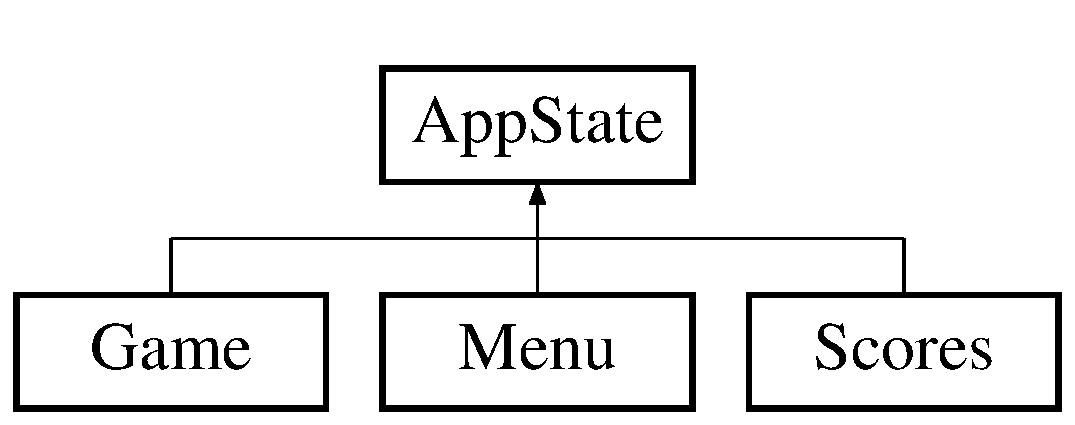
\includegraphics[height=2.000000cm]{class_app_state}
\end{center}
\end{figure}
\subsection*{Metody publiczne}
\begin{DoxyCompactItemize}
\item 
virtual \hyperlink{class_app_state_adef088013ce73c6c667f20a019b02d69}{$\sim$\+App\+State} ()
\item 
virtual bool \hyperlink{class_app_state_ad377464581817ae4000b9cd6c47dc4e8}{finished} () const =0
\item 
virtual void \hyperlink{class_app_state_ad2a668dc35b06c330a788e82d9eebee2}{draw} ()=0
\item 
virtual void \hyperlink{class_app_state_a28660de31b5a7a36691b67866f82e5f2}{update} (Uint32 dt)=0
\item 
virtual void \hyperlink{class_app_state_a9cd9175e5cd251bea2e7eeb4ee9f6137}{event\+Process} (S\+D\+L\+\_\+\+Event $\ast$ev)=0
\item 
virtual \hyperlink{class_app_state}{App\+State} $\ast$ \hyperlink{class_app_state_afafba64bbaaf7552f6e0632821c2338f}{next\+State} ()=0
\end{DoxyCompactItemize}


\subsection{Opis szczegółowy}
Klasa jest interfejsem, po którym dziedziczą klasy {\itshape \hyperlink{class_game}{Game}}, {\itshape \hyperlink{class_menu}{Menu}}, {\itshape \hyperlink{class_scores}{Scores}}. 

\subsection{Dokumentacja konstruktora i destruktora}
\hypertarget{class_app_state_adef088013ce73c6c667f20a019b02d69}{}\index{App\+State@{App\+State}!````~App\+State@{$\sim$\+App\+State}}
\index{````~App\+State@{$\sim$\+App\+State}!App\+State@{App\+State}}
\subsubsection[{$\sim$\+App\+State}]{\setlength{\rightskip}{0pt plus 5cm}virtual App\+State\+::$\sim$\+App\+State (
\begin{DoxyParamCaption}
{}
\end{DoxyParamCaption}
)\hspace{0.3cm}{\ttfamily [inline]}, {\ttfamily [virtual]}}\label{class_app_state_adef088013ce73c6c667f20a019b02d69}


\subsection{Dokumentacja funkcji składowych}
\hypertarget{class_app_state_ad2a668dc35b06c330a788e82d9eebee2}{}\index{App\+State@{App\+State}!draw@{draw}}
\index{draw@{draw}!App\+State@{App\+State}}
\subsubsection[{draw}]{\setlength{\rightskip}{0pt plus 5cm}virtual void App\+State\+::draw (
\begin{DoxyParamCaption}
{}
\end{DoxyParamCaption}
)\hspace{0.3cm}{\ttfamily [pure virtual]}}\label{class_app_state_ad2a668dc35b06c330a788e82d9eebee2}
Funkcja rysująca elementy gry należące do danego stanu 

Implementowany w \hyperlink{class_game_a6d54497ce3a66f6dd45eacfdccc8d0bd}{Game}, \hyperlink{class_menu_a2cd7ab9901a8f42a3ae977d0774398a6}{Menu} i \hyperlink{class_scores_a9fb6838fe10b06aa9f439e3aae90a803}{Scores}.

\hypertarget{class_app_state_a9cd9175e5cd251bea2e7eeb4ee9f6137}{}\index{App\+State@{App\+State}!event\+Process@{event\+Process}}
\index{event\+Process@{event\+Process}!App\+State@{App\+State}}
\subsubsection[{event\+Process}]{\setlength{\rightskip}{0pt plus 5cm}virtual void App\+State\+::event\+Process (
\begin{DoxyParamCaption}
\item[{S\+D\+L\+\_\+\+Event $\ast$}]{ev}
\end{DoxyParamCaption}
)\hspace{0.3cm}{\ttfamily [pure virtual]}}\label{class_app_state_a9cd9175e5cd251bea2e7eeb4ee9f6137}
Funkcja umożliwiająca obsługę zdarzeń wykrywanych przez bibliotekę S\+D\+L2. 
\begin{DoxyParams}{Parametry}
{\em ev} & -\/ wskaźnik na unię S\+D\+L\+\_\+\+Event przechowującą typ i parametry różnych zdarzeń \\
\hline
\end{DoxyParams}


Implementowany w \hyperlink{class_game_abd882b2a5629e55ac4df6d39a6f3311f}{Game}, \hyperlink{class_menu_a0b84052947f8687e10afe15ec88c90a9}{Menu} i \hyperlink{class_scores_ad6600e877a2b1c794cd1e849a7092d5e}{Scores}.

\hypertarget{class_app_state_ad377464581817ae4000b9cd6c47dc4e8}{}\index{App\+State@{App\+State}!finished@{finished}}
\index{finished@{finished}!App\+State@{App\+State}}
\subsubsection[{finished}]{\setlength{\rightskip}{0pt plus 5cm}virtual bool App\+State\+::finished (
\begin{DoxyParamCaption}
{}
\end{DoxyParamCaption}
) const\hspace{0.3cm}{\ttfamily [pure virtual]}}\label{class_app_state_ad377464581817ae4000b9cd6c47dc4e8}
Funkcja sprawdza czy aktualny stan gry się skończył. \begin{DoxyReturn}{Zwraca}
{\itshape true} jeżeli obecny stan gry się skończył, w przeciwnym wypadku {\itshape false}. 
\end{DoxyReturn}


Implementowany w \hyperlink{class_game_ad425f484c9b48d968ab76632fda9b2f3}{Game}, \hyperlink{class_menu_ac72d49b5565464340c2c25bd335c9424}{Menu} i \hyperlink{class_scores_ace5dca138217e9bc5b18871b9ea9764b}{Scores}.

\hypertarget{class_app_state_afafba64bbaaf7552f6e0632821c2338f}{}\index{App\+State@{App\+State}!next\+State@{next\+State}}
\index{next\+State@{next\+State}!App\+State@{App\+State}}
\subsubsection[{next\+State}]{\setlength{\rightskip}{0pt plus 5cm}virtual {\bf App\+State}$\ast$ App\+State\+::next\+State (
\begin{DoxyParamCaption}
{}
\end{DoxyParamCaption}
)\hspace{0.3cm}{\ttfamily [pure virtual]}}\label{class_app_state_afafba64bbaaf7552f6e0632821c2338f}
Funkcja zwracającya następny stan po zakończeniu obecnego. Funkcję należy wywołać tylko wtedy, gdy funkcja {\itshape finished} zwróci wartość 1. \begin{DoxyReturn}{Zwraca}
następny stan gry 
\end{DoxyReturn}


Implementowany w \hyperlink{class_game_a7dcc996fd972a30a8038c575a72ccaa2}{Game}, \hyperlink{class_menu_a52b14eefa8e7e9bee6624f759daa5028}{Menu} i \hyperlink{class_scores_abd664c78d44381251db40ebba0e5b773}{Scores}.

\hypertarget{class_app_state_a28660de31b5a7a36691b67866f82e5f2}{}\index{App\+State@{App\+State}!update@{update}}
\index{update@{update}!App\+State@{App\+State}}
\subsubsection[{update}]{\setlength{\rightskip}{0pt plus 5cm}virtual void App\+State\+::update (
\begin{DoxyParamCaption}
\item[{Uint32}]{dt}
\end{DoxyParamCaption}
)\hspace{0.3cm}{\ttfamily [pure virtual]}}\label{class_app_state_a28660de31b5a7a36691b67866f82e5f2}
Funkcja aktualizująca stan obiektów i liczników w grze 
\begin{DoxyParams}{Parametry}
{\em dt} & -\/ czas od ostatniego wywołania funkcji w milisekundach \\
\hline
\end{DoxyParams}


Implementowany w \hyperlink{class_game_a502c1be9a7afadbfc679d501034c7b4a}{Game}, \hyperlink{class_menu_a02ff964c4a203ca08b11655c36252fc8}{Menu} i \hyperlink{class_scores_ae1eda4aec4cfc65c8bacb648ea28212e}{Scores}.



Dokumentacja dla tej klasy została wygenerowana z pliku\+:\begin{DoxyCompactItemize}
\item 
src/app\+\_\+state/\hyperlink{appstate_8h}{appstate.\+h}\end{DoxyCompactItemize}

\hypertarget{class_bonus}{}\section{Dokumentacja klasy Bonus}
\label{class_bonus}\index{Bonus@{Bonus}}


{\ttfamily \#include $<$bonus.\+h$>$}

Diagram dziedziczenia dla Bonus\begin{figure}[H]
\begin{center}
\leavevmode
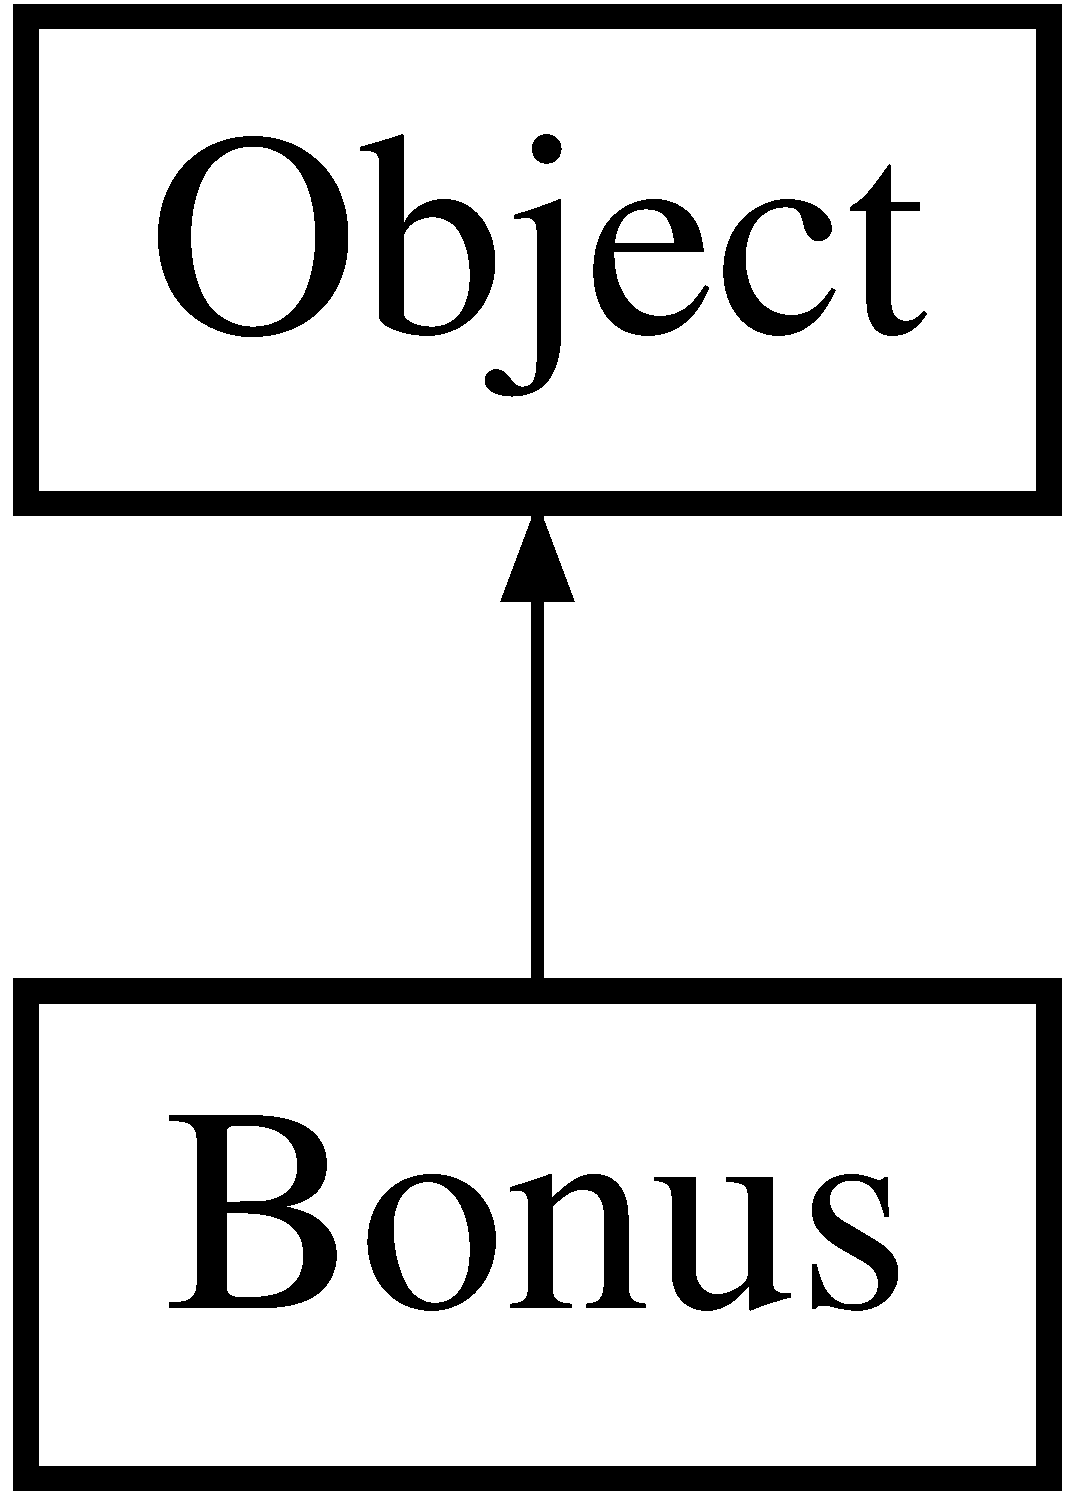
\includegraphics[height=2.000000cm]{class_bonus}
\end{center}
\end{figure}
\subsection*{Metody publiczne}
\begin{DoxyCompactItemize}
\item 
\hyperlink{class_bonus_a005571f0961a2e0f1af2befc35d804cf}{Bonus} ()
\item 
\hyperlink{class_bonus_ac7874d08071f7ffcbed3ea1140c2f385}{Bonus} (double x, double y, \hyperlink{type_8h_ac6fa10729dffeb6a192492f13c25e31a}{Sprite\+Type} \hyperlink{class_object_a1b89f32cd9e0040f8a2455f3cef7d0d2}{type})
\item 
void \hyperlink{class_bonus_a00a6ad75da471b6a577029be0b80e259}{draw} ()
\item 
void \hyperlink{class_bonus_a53c7235c0dae0deddfc95a2b7c5a594b}{update} (Uint32 dt)
\end{DoxyCompactItemize}
\subsection*{Dodatkowe Dziedziczone Składowe}


\subsection{Dokumentacja konstruktora i destruktora}
\hypertarget{class_bonus_a005571f0961a2e0f1af2befc35d804cf}{}\index{Bonus@{Bonus}!Bonus@{Bonus}}
\index{Bonus@{Bonus}!Bonus@{Bonus}}
\subsubsection[{Bonus}]{\setlength{\rightskip}{0pt plus 5cm}Bonus\+::\+Bonus (
\begin{DoxyParamCaption}
{}
\end{DoxyParamCaption}
)}\label{class_bonus_a005571f0961a2e0f1af2befc35d804cf}
\hypertarget{class_bonus_ac7874d08071f7ffcbed3ea1140c2f385}{}\index{Bonus@{Bonus}!Bonus@{Bonus}}
\index{Bonus@{Bonus}!Bonus@{Bonus}}
\subsubsection[{Bonus}]{\setlength{\rightskip}{0pt plus 5cm}Bonus\+::\+Bonus (
\begin{DoxyParamCaption}
\item[{double}]{x, }
\item[{double}]{y, }
\item[{{\bf Sprite\+Type}}]{type}
\end{DoxyParamCaption}
)}\label{class_bonus_ac7874d08071f7ffcbed3ea1140c2f385}


\subsection{Dokumentacja funkcji składowych}
\hypertarget{class_bonus_a00a6ad75da471b6a577029be0b80e259}{}\index{Bonus@{Bonus}!draw@{draw}}
\index{draw@{draw}!Bonus@{Bonus}}
\subsubsection[{draw}]{\setlength{\rightskip}{0pt plus 5cm}void Bonus\+::draw (
\begin{DoxyParamCaption}
{}
\end{DoxyParamCaption}
)\hspace{0.3cm}{\ttfamily [virtual]}}\label{class_bonus_a00a6ad75da471b6a577029be0b80e259}


Reimplementowana z \hyperlink{class_object_a821f5b25b450fa1acdb3f9c0b5962592}{Object}.

\hypertarget{class_bonus_a53c7235c0dae0deddfc95a2b7c5a594b}{}\index{Bonus@{Bonus}!update@{update}}
\index{update@{update}!Bonus@{Bonus}}
\subsubsection[{update}]{\setlength{\rightskip}{0pt plus 5cm}void Bonus\+::update (
\begin{DoxyParamCaption}
\item[{Uint32}]{dt}
\end{DoxyParamCaption}
)\hspace{0.3cm}{\ttfamily [virtual]}}\label{class_bonus_a53c7235c0dae0deddfc95a2b7c5a594b}


Reimplementowana z \hyperlink{class_object_a02c1621329cb9ec5268072a2402d2ac5}{Object}.



Dokumentacja dla tej klasy została wygenerowana z plików\+:\begin{DoxyCompactItemize}
\item 
src/objects/\hyperlink{bonus_8h}{bonus.\+h}\item 
src/objects/\hyperlink{bonus_8cpp}{bonus.\+cpp}\end{DoxyCompactItemize}

\hypertarget{class_brick}{}\section{Dokumentacja klasy Brick}
\label{class_brick}\index{Brick@{Brick}}


{\ttfamily \#include $<$brick.\+h$>$}

Diagram dziedziczenia dla Brick\begin{figure}[H]
\begin{center}
\leavevmode
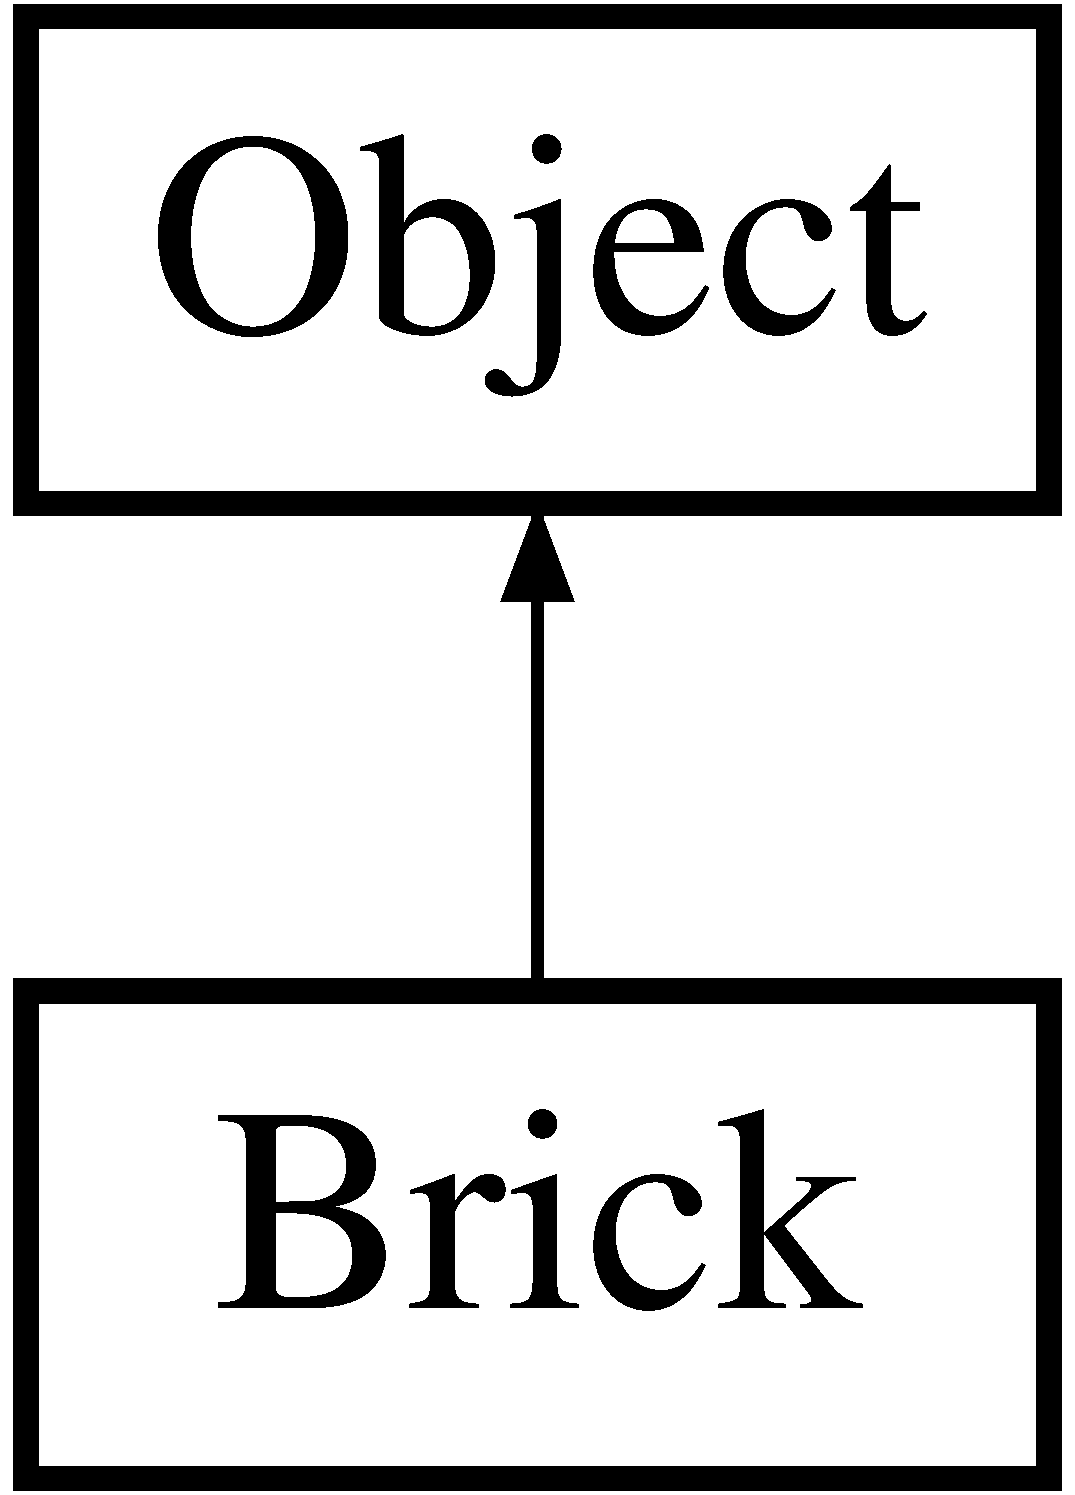
\includegraphics[height=2.000000cm]{class_brick}
\end{center}
\end{figure}
\subsection*{Metody publiczne}
\begin{DoxyCompactItemize}
\item 
\hyperlink{class_brick_aa29d678c3d901c7b18cbc3a27a51be17}{Brick} ()
\item 
\hyperlink{class_brick_afd3f1b7ddb33853509c0820542d68b1e}{Brick} (double x, double y)
\item 
void \hyperlink{class_brick_a31098851b4f1224cfd6b51c4ef47094f}{update} (Uint32 dt)
\item 
void \hyperlink{class_brick_a9cc85dce3b78ecd20737e3eda8731b31}{bullet\+Hit} (\hyperlink{type_8h_a224b9163917ac32fc95a60d8c1eec3aa}{Direction} bullet\+\_\+direction)
\end{DoxyCompactItemize}
\subsection*{Dodatkowe Dziedziczone Składowe}


\subsection{Dokumentacja konstruktora i destruktora}
\hypertarget{class_brick_aa29d678c3d901c7b18cbc3a27a51be17}{}\index{Brick@{Brick}!Brick@{Brick}}
\index{Brick@{Brick}!Brick@{Brick}}
\subsubsection[{Brick}]{\setlength{\rightskip}{0pt plus 5cm}Brick\+::\+Brick (
\begin{DoxyParamCaption}
{}
\end{DoxyParamCaption}
)}\label{class_brick_aa29d678c3d901c7b18cbc3a27a51be17}
\hypertarget{class_brick_afd3f1b7ddb33853509c0820542d68b1e}{}\index{Brick@{Brick}!Brick@{Brick}}
\index{Brick@{Brick}!Brick@{Brick}}
\subsubsection[{Brick}]{\setlength{\rightskip}{0pt plus 5cm}Brick\+::\+Brick (
\begin{DoxyParamCaption}
\item[{double}]{x, }
\item[{double}]{y}
\end{DoxyParamCaption}
)}\label{class_brick_afd3f1b7ddb33853509c0820542d68b1e}


\subsection{Dokumentacja funkcji składowych}
\hypertarget{class_brick_a9cc85dce3b78ecd20737e3eda8731b31}{}\index{Brick@{Brick}!bullet\+Hit@{bullet\+Hit}}
\index{bullet\+Hit@{bullet\+Hit}!Brick@{Brick}}
\subsubsection[{bullet\+Hit}]{\setlength{\rightskip}{0pt plus 5cm}void Brick\+::bullet\+Hit (
\begin{DoxyParamCaption}
\item[{{\bf Direction}}]{bullet\+\_\+direction}
\end{DoxyParamCaption}
)}\label{class_brick_a9cc85dce3b78ecd20737e3eda8731b31}
\hypertarget{class_brick_a31098851b4f1224cfd6b51c4ef47094f}{}\index{Brick@{Brick}!update@{update}}
\index{update@{update}!Brick@{Brick}}
\subsubsection[{update}]{\setlength{\rightskip}{0pt plus 5cm}void Brick\+::update (
\begin{DoxyParamCaption}
\item[{Uint32}]{dt}
\end{DoxyParamCaption}
)\hspace{0.3cm}{\ttfamily [virtual]}}\label{class_brick_a31098851b4f1224cfd6b51c4ef47094f}


Reimplementowana z \hyperlink{class_object_a02c1621329cb9ec5268072a2402d2ac5}{Object}.



Dokumentacja dla tej klasy została wygenerowana z plików\+:\begin{DoxyCompactItemize}
\item 
src/objects/\hyperlink{brick_8h}{brick.\+h}\item 
src/objects/\hyperlink{brick_8cpp}{brick.\+cpp}\end{DoxyCompactItemize}

\hypertarget{class_bullet}{}\section{Dokumentacja klasy Bullet}
\label{class_bullet}\index{Bullet@{Bullet}}


{\ttfamily \#include $<$bullet.\+h$>$}

Diagram dziedziczenia dla Bullet\begin{figure}[H]
\begin{center}
\leavevmode
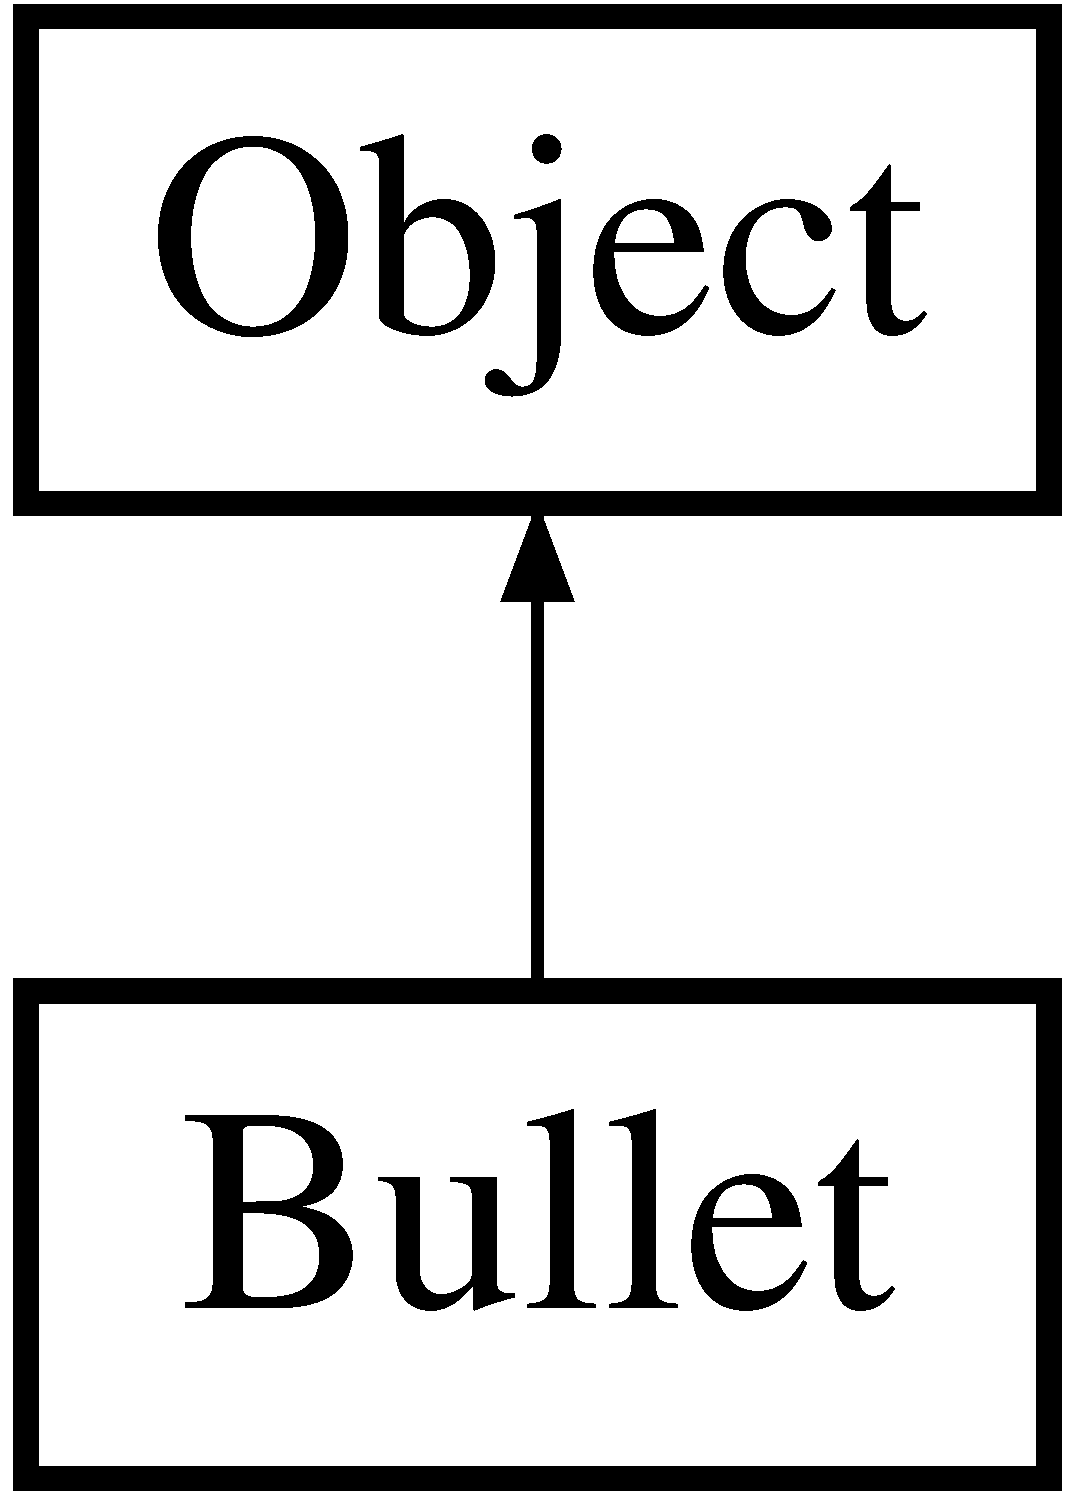
\includegraphics[height=2.000000cm]{class_bullet}
\end{center}
\end{figure}
\subsection*{Metody publiczne}
\begin{DoxyCompactItemize}
\item 
\hyperlink{class_bullet_acd7befc0bc18907cc1d871d37bbdddeb}{Bullet} ()
\item 
\hyperlink{class_bullet_ae40cb12a4475a5a9023fbe46d35433ab}{Bullet} (double x, double y)
\item 
void \hyperlink{class_bullet_a28c27c103a23f73d18125791c973cccd}{update} (Uint32 dt)
\item 
void \hyperlink{class_bullet_a688d6b75822e4cab5f1cbcdd1511263a}{destroy} ()
\end{DoxyCompactItemize}
\subsection*{Atrybuty publiczne}
\begin{DoxyCompactItemize}
\item 
double \hyperlink{class_bullet_aa610411cbf6fd6fa3d744c3f85c8de9f}{speed}
\item 
bool \hyperlink{class_bullet_a13bf4d55e52ef924643268607bb0db4f}{collide}
\item 
bool \hyperlink{class_bullet_a646bf8c94671a65133901b73325898d4}{increased\+\_\+damage}
\item 
\hyperlink{type_8h_a224b9163917ac32fc95a60d8c1eec3aa}{Direction} \hyperlink{class_bullet_a8a97d74eabfadabaec346a98c6b67b0e}{direction}
\end{DoxyCompactItemize}
\subsection*{Dodatkowe Dziedziczone Składowe}


\subsection{Dokumentacja konstruktora i destruktora}
\hypertarget{class_bullet_acd7befc0bc18907cc1d871d37bbdddeb}{}\index{Bullet@{Bullet}!Bullet@{Bullet}}
\index{Bullet@{Bullet}!Bullet@{Bullet}}
\subsubsection[{Bullet}]{\setlength{\rightskip}{0pt plus 5cm}Bullet\+::\+Bullet (
\begin{DoxyParamCaption}
{}
\end{DoxyParamCaption}
)}\label{class_bullet_acd7befc0bc18907cc1d871d37bbdddeb}
\hypertarget{class_bullet_ae40cb12a4475a5a9023fbe46d35433ab}{}\index{Bullet@{Bullet}!Bullet@{Bullet}}
\index{Bullet@{Bullet}!Bullet@{Bullet}}
\subsubsection[{Bullet}]{\setlength{\rightskip}{0pt plus 5cm}Bullet\+::\+Bullet (
\begin{DoxyParamCaption}
\item[{double}]{x, }
\item[{double}]{y}
\end{DoxyParamCaption}
)}\label{class_bullet_ae40cb12a4475a5a9023fbe46d35433ab}


\subsection{Dokumentacja funkcji składowych}
\hypertarget{class_bullet_a688d6b75822e4cab5f1cbcdd1511263a}{}\index{Bullet@{Bullet}!destroy@{destroy}}
\index{destroy@{destroy}!Bullet@{Bullet}}
\subsubsection[{destroy}]{\setlength{\rightskip}{0pt plus 5cm}void Bullet\+::destroy (
\begin{DoxyParamCaption}
{}
\end{DoxyParamCaption}
)}\label{class_bullet_a688d6b75822e4cab5f1cbcdd1511263a}
\hypertarget{class_bullet_a28c27c103a23f73d18125791c973cccd}{}\index{Bullet@{Bullet}!update@{update}}
\index{update@{update}!Bullet@{Bullet}}
\subsubsection[{update}]{\setlength{\rightskip}{0pt plus 5cm}void Bullet\+::update (
\begin{DoxyParamCaption}
\item[{Uint32}]{dt}
\end{DoxyParamCaption}
)\hspace{0.3cm}{\ttfamily [virtual]}}\label{class_bullet_a28c27c103a23f73d18125791c973cccd}


Reimplementowana z \hyperlink{class_object_a02c1621329cb9ec5268072a2402d2ac5}{Object}.



\subsection{Dokumentacja atrybutów składowych}
\hypertarget{class_bullet_a13bf4d55e52ef924643268607bb0db4f}{}\index{Bullet@{Bullet}!collide@{collide}}
\index{collide@{collide}!Bullet@{Bullet}}
\subsubsection[{collide}]{\setlength{\rightskip}{0pt plus 5cm}bool Bullet\+::collide}\label{class_bullet_a13bf4d55e52ef924643268607bb0db4f}
\hypertarget{class_bullet_a8a97d74eabfadabaec346a98c6b67b0e}{}\index{Bullet@{Bullet}!direction@{direction}}
\index{direction@{direction}!Bullet@{Bullet}}
\subsubsection[{direction}]{\setlength{\rightskip}{0pt plus 5cm}{\bf Direction} Bullet\+::direction}\label{class_bullet_a8a97d74eabfadabaec346a98c6b67b0e}
\hypertarget{class_bullet_a646bf8c94671a65133901b73325898d4}{}\index{Bullet@{Bullet}!increased\+\_\+damage@{increased\+\_\+damage}}
\index{increased\+\_\+damage@{increased\+\_\+damage}!Bullet@{Bullet}}
\subsubsection[{increased\+\_\+damage}]{\setlength{\rightskip}{0pt plus 5cm}bool Bullet\+::increased\+\_\+damage}\label{class_bullet_a646bf8c94671a65133901b73325898d4}
\hypertarget{class_bullet_aa610411cbf6fd6fa3d744c3f85c8de9f}{}\index{Bullet@{Bullet}!speed@{speed}}
\index{speed@{speed}!Bullet@{Bullet}}
\subsubsection[{speed}]{\setlength{\rightskip}{0pt plus 5cm}double Bullet\+::speed}\label{class_bullet_aa610411cbf6fd6fa3d744c3f85c8de9f}


Dokumentacja dla tej klasy została wygenerowana z plików\+:\begin{DoxyCompactItemize}
\item 
src/objects/\hyperlink{bullet_8h}{bullet.\+h}\item 
src/objects/\hyperlink{bullet_8cpp}{bullet.\+cpp}\end{DoxyCompactItemize}

\hypertarget{class_eagle}{}\section{Dokumentacja klasy Eagle}
\label{class_eagle}\index{Eagle@{Eagle}}


{\ttfamily \#include $<$eagle.\+h$>$}

Diagram dziedziczenia dla Eagle\begin{figure}[H]
\begin{center}
\leavevmode
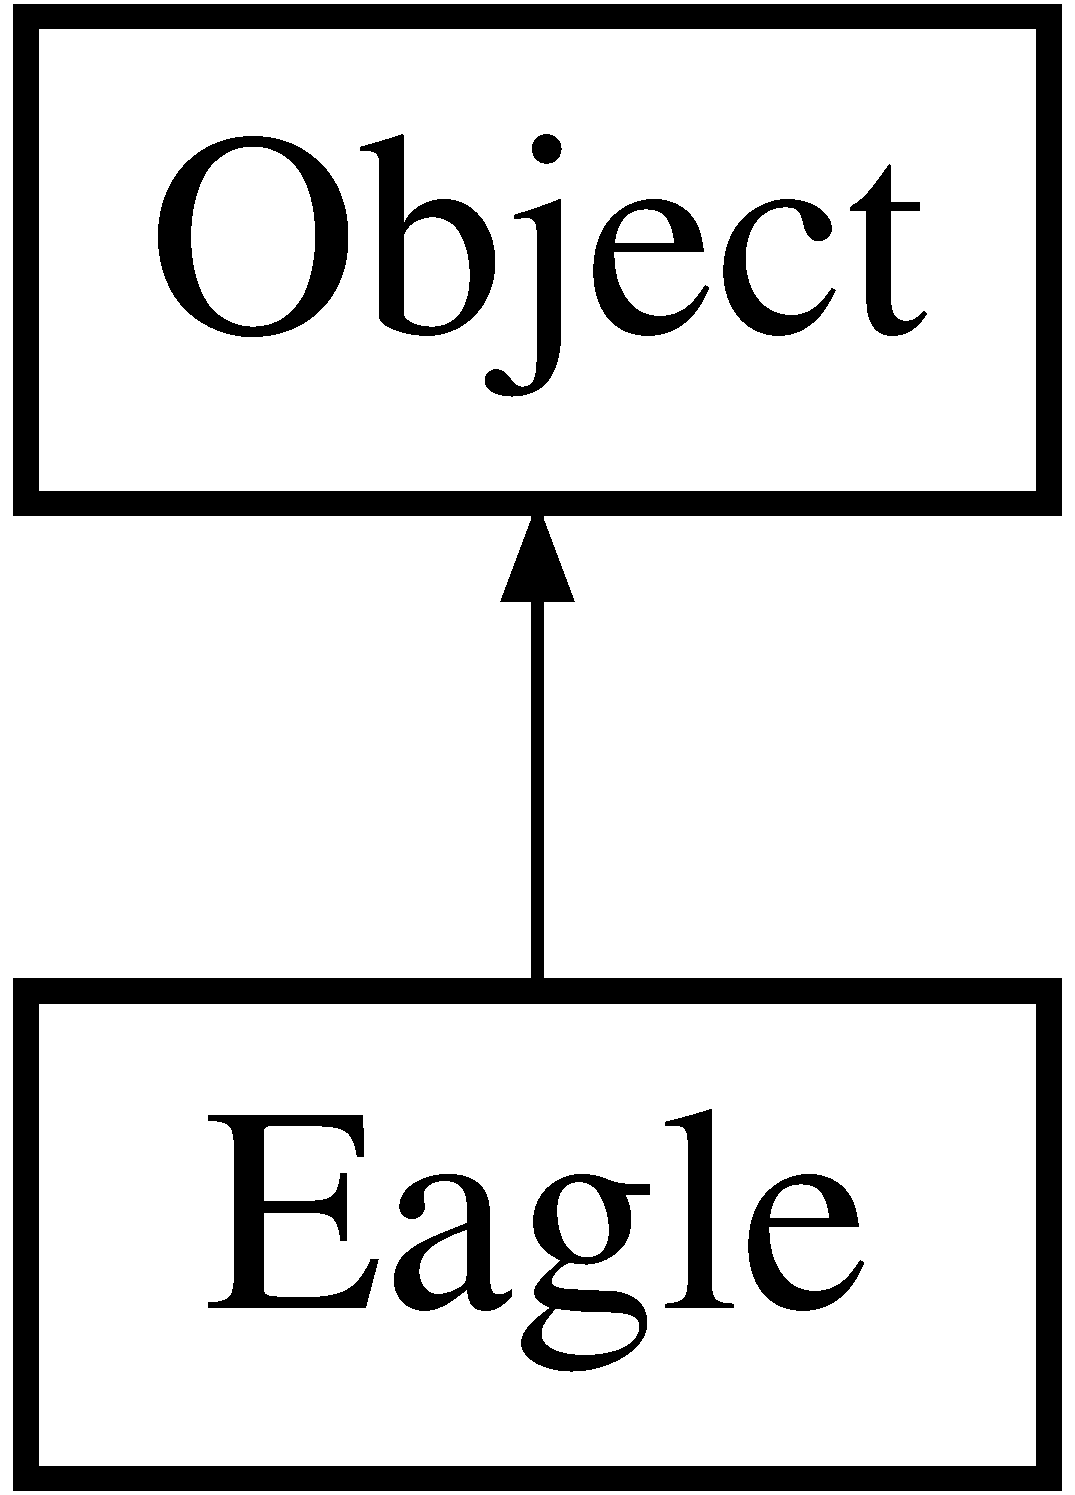
\includegraphics[height=2.000000cm]{class_eagle}
\end{center}
\end{figure}
\subsection*{Metody publiczne}
\begin{DoxyCompactItemize}
\item 
\hyperlink{class_eagle_a8b205e5b26bece07d18b852b042851fe}{Eagle} ()
\item 
\hyperlink{class_eagle_a31ccd219369751a36a30bfaf498beb2e}{Eagle} (double x, double y)
\item 
void \hyperlink{class_eagle_a609e173a641783b14973d5e1055f192a}{update} (Uint32 dt)
\item 
void \hyperlink{class_eagle_a655a8119eb862168d8cc8b04ace23aa5}{destroy} ()
\end{DoxyCompactItemize}
\subsection*{Dodatkowe Dziedziczone Składowe}


\subsection{Dokumentacja konstruktora i destruktora}
\hypertarget{class_eagle_a8b205e5b26bece07d18b852b042851fe}{}\index{Eagle@{Eagle}!Eagle@{Eagle}}
\index{Eagle@{Eagle}!Eagle@{Eagle}}
\subsubsection[{Eagle}]{\setlength{\rightskip}{0pt plus 5cm}Eagle\+::\+Eagle (
\begin{DoxyParamCaption}
{}
\end{DoxyParamCaption}
)}\label{class_eagle_a8b205e5b26bece07d18b852b042851fe}
\hypertarget{class_eagle_a31ccd219369751a36a30bfaf498beb2e}{}\index{Eagle@{Eagle}!Eagle@{Eagle}}
\index{Eagle@{Eagle}!Eagle@{Eagle}}
\subsubsection[{Eagle}]{\setlength{\rightskip}{0pt plus 5cm}Eagle\+::\+Eagle (
\begin{DoxyParamCaption}
\item[{double}]{x, }
\item[{double}]{y}
\end{DoxyParamCaption}
)}\label{class_eagle_a31ccd219369751a36a30bfaf498beb2e}


\subsection{Dokumentacja funkcji składowych}
\hypertarget{class_eagle_a655a8119eb862168d8cc8b04ace23aa5}{}\index{Eagle@{Eagle}!destroy@{destroy}}
\index{destroy@{destroy}!Eagle@{Eagle}}
\subsubsection[{destroy}]{\setlength{\rightskip}{0pt plus 5cm}void Eagle\+::destroy (
\begin{DoxyParamCaption}
{}
\end{DoxyParamCaption}
)}\label{class_eagle_a655a8119eb862168d8cc8b04ace23aa5}
\hypertarget{class_eagle_a609e173a641783b14973d5e1055f192a}{}\index{Eagle@{Eagle}!update@{update}}
\index{update@{update}!Eagle@{Eagle}}
\subsubsection[{update}]{\setlength{\rightskip}{0pt plus 5cm}void Eagle\+::update (
\begin{DoxyParamCaption}
\item[{Uint32}]{dt}
\end{DoxyParamCaption}
)\hspace{0.3cm}{\ttfamily [virtual]}}\label{class_eagle_a609e173a641783b14973d5e1055f192a}


Reimplementowana z \hyperlink{class_object_a02c1621329cb9ec5268072a2402d2ac5}{Object}.



Dokumentacja dla tej klasy została wygenerowana z plików\+:\begin{DoxyCompactItemize}
\item 
src/objects/\hyperlink{eagle_8h}{eagle.\+h}\item 
src/objects/\hyperlink{eagle_8cpp}{eagle.\+cpp}\end{DoxyCompactItemize}

\hypertarget{class_enemy}{}\section{Dokumentacja klasy Enemy}
\label{class_enemy}\index{Enemy@{Enemy}}


{\ttfamily \#include $<$enemy.\+h$>$}

Diagram dziedziczenia dla Enemy\begin{figure}[H]
\begin{center}
\leavevmode
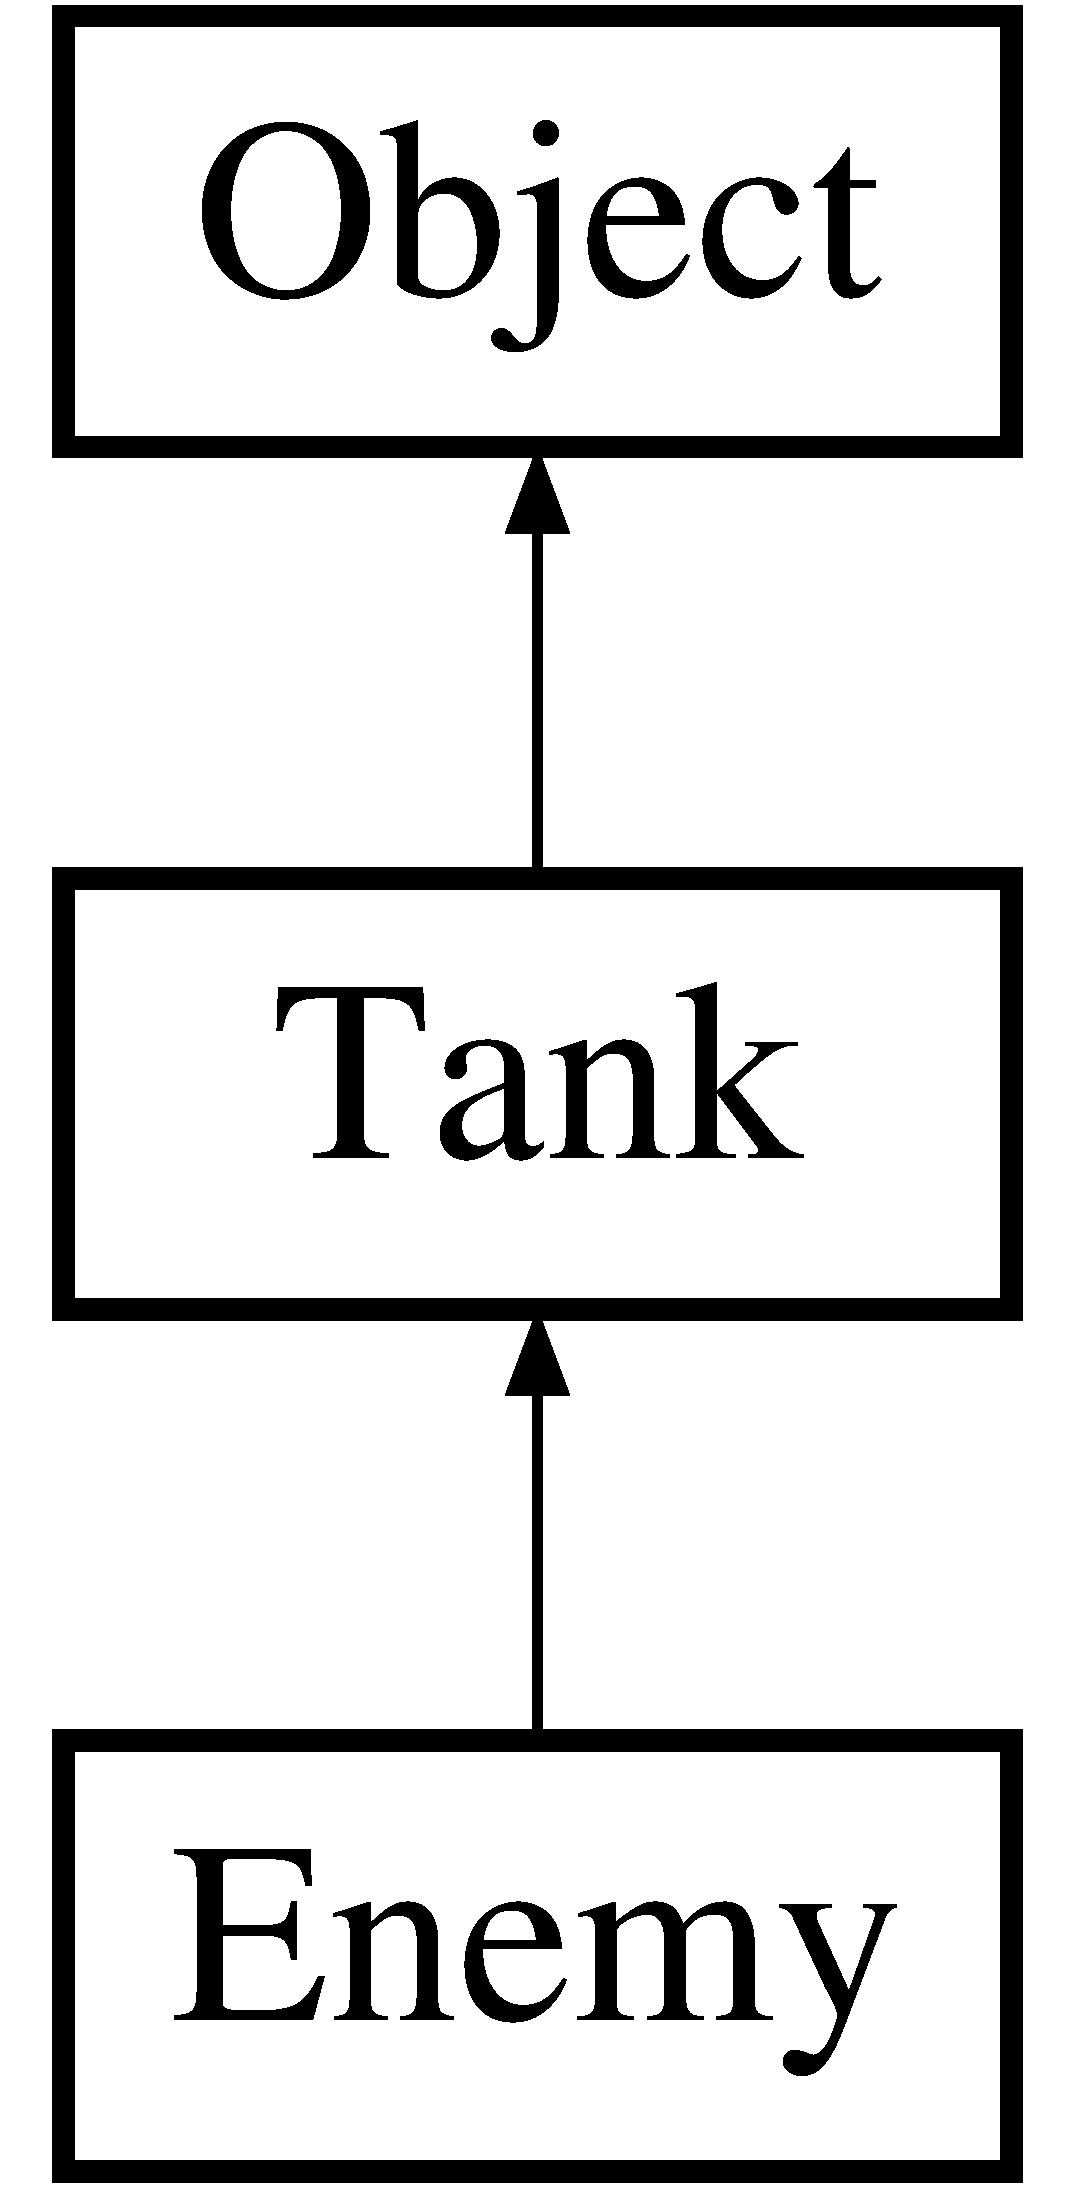
\includegraphics[height=3.000000cm]{class_enemy}
\end{center}
\end{figure}
\subsection*{Metody publiczne}
\begin{DoxyCompactItemize}
\item 
\hyperlink{class_enemy_a94f30d348b6d2840fd71675472ba38dd}{Enemy} ()
\item 
\hyperlink{class_enemy_a716fd77723d2c3c9a521672245bf89f8}{Enemy} (double x, double y, \hyperlink{type_8h_ac6fa10729dffeb6a192492f13c25e31a}{Sprite\+Type} \hyperlink{class_object_a1b89f32cd9e0040f8a2455f3cef7d0d2}{type})
\item 
void \hyperlink{class_enemy_a7dcf45915f6288ef9264ec60af621b6c}{draw} ()
\item 
void \hyperlink{class_enemy_a03c09cab6c4950e4cae880c15b2fd739}{update} (Uint32 dt)
\item 
void \hyperlink{class_enemy_a296a5757097f271eb01284eabb064715}{destroy} ()
\item 
unsigned \hyperlink{class_enemy_a024794c12555ca3b948aebb576e8915e}{score\+For\+Hit} ()
\end{DoxyCompactItemize}
\subsection*{Atrybuty publiczne}
\begin{DoxyCompactItemize}
\item 
S\+D\+L\+\_\+\+Point \hyperlink{class_enemy_abb410f03f34e4a1ce889ef8441382eb0}{target\+\_\+position}
\end{DoxyCompactItemize}
\subsection*{Dodatkowe Dziedziczone Składowe}


\subsection{Dokumentacja konstruktora i destruktora}
\hypertarget{class_enemy_a94f30d348b6d2840fd71675472ba38dd}{}\index{Enemy@{Enemy}!Enemy@{Enemy}}
\index{Enemy@{Enemy}!Enemy@{Enemy}}
\subsubsection[{Enemy}]{\setlength{\rightskip}{0pt plus 5cm}Enemy\+::\+Enemy (
\begin{DoxyParamCaption}
{}
\end{DoxyParamCaption}
)}\label{class_enemy_a94f30d348b6d2840fd71675472ba38dd}
\hypertarget{class_enemy_a716fd77723d2c3c9a521672245bf89f8}{}\index{Enemy@{Enemy}!Enemy@{Enemy}}
\index{Enemy@{Enemy}!Enemy@{Enemy}}
\subsubsection[{Enemy}]{\setlength{\rightskip}{0pt plus 5cm}Enemy\+::\+Enemy (
\begin{DoxyParamCaption}
\item[{double}]{x, }
\item[{double}]{y, }
\item[{{\bf Sprite\+Type}}]{type}
\end{DoxyParamCaption}
)}\label{class_enemy_a716fd77723d2c3c9a521672245bf89f8}


\subsection{Dokumentacja funkcji składowych}
\hypertarget{class_enemy_a296a5757097f271eb01284eabb064715}{}\index{Enemy@{Enemy}!destroy@{destroy}}
\index{destroy@{destroy}!Enemy@{Enemy}}
\subsubsection[{destroy}]{\setlength{\rightskip}{0pt plus 5cm}void Enemy\+::destroy (
\begin{DoxyParamCaption}
{}
\end{DoxyParamCaption}
)\hspace{0.3cm}{\ttfamily [virtual]}}\label{class_enemy_a296a5757097f271eb01284eabb064715}


Reimplementowana z \hyperlink{class_tank_a5d2e3302417166ccdc42b8bc2e5d5dc4}{Tank}.

\hypertarget{class_enemy_a7dcf45915f6288ef9264ec60af621b6c}{}\index{Enemy@{Enemy}!draw@{draw}}
\index{draw@{draw}!Enemy@{Enemy}}
\subsubsection[{draw}]{\setlength{\rightskip}{0pt plus 5cm}void Enemy\+::draw (
\begin{DoxyParamCaption}
{}
\end{DoxyParamCaption}
)\hspace{0.3cm}{\ttfamily [virtual]}}\label{class_enemy_a7dcf45915f6288ef9264ec60af621b6c}


Reimplementowana z \hyperlink{class_object_a821f5b25b450fa1acdb3f9c0b5962592}{Object}.

\hypertarget{class_enemy_a024794c12555ca3b948aebb576e8915e}{}\index{Enemy@{Enemy}!score\+For\+Hit@{score\+For\+Hit}}
\index{score\+For\+Hit@{score\+For\+Hit}!Enemy@{Enemy}}
\subsubsection[{score\+For\+Hit}]{\setlength{\rightskip}{0pt plus 5cm}unsigned Enemy\+::score\+For\+Hit (
\begin{DoxyParamCaption}
{}
\end{DoxyParamCaption}
)}\label{class_enemy_a024794c12555ca3b948aebb576e8915e}
\hypertarget{class_enemy_a03c09cab6c4950e4cae880c15b2fd739}{}\index{Enemy@{Enemy}!update@{update}}
\index{update@{update}!Enemy@{Enemy}}
\subsubsection[{update}]{\setlength{\rightskip}{0pt plus 5cm}void Enemy\+::update (
\begin{DoxyParamCaption}
\item[{Uint32}]{dt}
\end{DoxyParamCaption}
)\hspace{0.3cm}{\ttfamily [virtual]}}\label{class_enemy_a03c09cab6c4950e4cae880c15b2fd739}


Reimplementowana z \hyperlink{class_object_a02c1621329cb9ec5268072a2402d2ac5}{Object}.



\subsection{Dokumentacja atrybutów składowych}
\hypertarget{class_enemy_abb410f03f34e4a1ce889ef8441382eb0}{}\index{Enemy@{Enemy}!target\+\_\+position@{target\+\_\+position}}
\index{target\+\_\+position@{target\+\_\+position}!Enemy@{Enemy}}
\subsubsection[{target\+\_\+position}]{\setlength{\rightskip}{0pt plus 5cm}S\+D\+L\+\_\+\+Point Enemy\+::target\+\_\+position}\label{class_enemy_abb410f03f34e4a1ce889ef8441382eb0}


Dokumentacja dla tej klasy została wygenerowana z plików\+:\begin{DoxyCompactItemize}
\item 
src/objects/\hyperlink{enemy_8h}{enemy.\+h}\item 
src/objects/\hyperlink{enemy_8cpp}{enemy.\+cpp}\end{DoxyCompactItemize}

\hypertarget{class_engine}{}\section{Dokumentacja klasy Engine}
\label{class_engine}\index{Engine@{Engine}}


{\ttfamily \#include $<$engine.\+h$>$}

\subsection*{Metody publiczne}
\begin{DoxyCompactItemize}
\item 
\hyperlink{class_engine_a8c98683b0a3aa28d8ab72a8bcd0d52f2}{Engine} ()
\item 
void \hyperlink{class_engine_a36373d0a55fdf222623660c6c7b60d2f}{init\+Modules} ()
\item 
void \hyperlink{class_engine_a463522f735aa34310b38ef66a7ba766f}{destroy\+Modules} ()
\item 
\hyperlink{class_renderer}{Renderer} $\ast$ \hyperlink{class_engine_a4ae702a17d6ca093ea6d2bbe37494805}{get\+Renderer} () const 
\item 
\hyperlink{class_sprite_config}{Sprite\+Config} $\ast$ \hyperlink{class_engine_add1c56f65b2ae1cee44d31a4e60559f3}{get\+Sprite\+Config} () const 
\end{DoxyCompactItemize}
\subsection*{Statyczne metody publiczne}
\begin{DoxyCompactItemize}
\item 
static \hyperlink{class_engine}{Engine} \& \hyperlink{class_engine_a2fdd20971d12ee816899854c05d8ed9b}{get\+Engine} ()
\item 
static std\+::string \hyperlink{class_engine_a7aeb45fda14d92d4310eb7ec0f5af432}{int\+To\+String} (int num)
\end{DoxyCompactItemize}


\subsection{Dokumentacja konstruktora i destruktora}
\hypertarget{class_engine_a8c98683b0a3aa28d8ab72a8bcd0d52f2}{}\index{Engine@{Engine}!Engine@{Engine}}
\index{Engine@{Engine}!Engine@{Engine}}
\subsubsection[{Engine}]{\setlength{\rightskip}{0pt plus 5cm}Engine\+::\+Engine (
\begin{DoxyParamCaption}
{}
\end{DoxyParamCaption}
)}\label{class_engine_a8c98683b0a3aa28d8ab72a8bcd0d52f2}


\subsection{Dokumentacja funkcji składowych}
\hypertarget{class_engine_a463522f735aa34310b38ef66a7ba766f}{}\index{Engine@{Engine}!destroy\+Modules@{destroy\+Modules}}
\index{destroy\+Modules@{destroy\+Modules}!Engine@{Engine}}
\subsubsection[{destroy\+Modules}]{\setlength{\rightskip}{0pt plus 5cm}void Engine\+::destroy\+Modules (
\begin{DoxyParamCaption}
{}
\end{DoxyParamCaption}
)}\label{class_engine_a463522f735aa34310b38ef66a7ba766f}
\hypertarget{class_engine_a2fdd20971d12ee816899854c05d8ed9b}{}\index{Engine@{Engine}!get\+Engine@{get\+Engine}}
\index{get\+Engine@{get\+Engine}!Engine@{Engine}}
\subsubsection[{get\+Engine}]{\setlength{\rightskip}{0pt plus 5cm}{\bf Engine} \& Engine\+::get\+Engine (
\begin{DoxyParamCaption}
{}
\end{DoxyParamCaption}
)\hspace{0.3cm}{\ttfamily [static]}}\label{class_engine_a2fdd20971d12ee816899854c05d8ed9b}
\hypertarget{class_engine_a4ae702a17d6ca093ea6d2bbe37494805}{}\index{Engine@{Engine}!get\+Renderer@{get\+Renderer}}
\index{get\+Renderer@{get\+Renderer}!Engine@{Engine}}
\subsubsection[{get\+Renderer}]{\setlength{\rightskip}{0pt plus 5cm}{\bf Renderer} $\ast$ Engine\+::get\+Renderer (
\begin{DoxyParamCaption}
{}
\end{DoxyParamCaption}
) const}\label{class_engine_a4ae702a17d6ca093ea6d2bbe37494805}
\hypertarget{class_engine_add1c56f65b2ae1cee44d31a4e60559f3}{}\index{Engine@{Engine}!get\+Sprite\+Config@{get\+Sprite\+Config}}
\index{get\+Sprite\+Config@{get\+Sprite\+Config}!Engine@{Engine}}
\subsubsection[{get\+Sprite\+Config}]{\setlength{\rightskip}{0pt plus 5cm}{\bf Sprite\+Config} $\ast$ Engine\+::get\+Sprite\+Config (
\begin{DoxyParamCaption}
{}
\end{DoxyParamCaption}
) const}\label{class_engine_add1c56f65b2ae1cee44d31a4e60559f3}
\hypertarget{class_engine_a36373d0a55fdf222623660c6c7b60d2f}{}\index{Engine@{Engine}!init\+Modules@{init\+Modules}}
\index{init\+Modules@{init\+Modules}!Engine@{Engine}}
\subsubsection[{init\+Modules}]{\setlength{\rightskip}{0pt plus 5cm}void Engine\+::init\+Modules (
\begin{DoxyParamCaption}
{}
\end{DoxyParamCaption}
)}\label{class_engine_a36373d0a55fdf222623660c6c7b60d2f}
\hypertarget{class_engine_a7aeb45fda14d92d4310eb7ec0f5af432}{}\index{Engine@{Engine}!int\+To\+String@{int\+To\+String}}
\index{int\+To\+String@{int\+To\+String}!Engine@{Engine}}
\subsubsection[{int\+To\+String}]{\setlength{\rightskip}{0pt plus 5cm}std\+::string Engine\+::int\+To\+String (
\begin{DoxyParamCaption}
\item[{int}]{num}
\end{DoxyParamCaption}
)\hspace{0.3cm}{\ttfamily [static]}}\label{class_engine_a7aeb45fda14d92d4310eb7ec0f5af432}


Dokumentacja dla tej klasy została wygenerowana z plików\+:\begin{DoxyCompactItemize}
\item 
src/engine/\hyperlink{engine_8h}{engine.\+h}\item 
src/engine/\hyperlink{engine_8cpp}{engine.\+cpp}\end{DoxyCompactItemize}

\hypertarget{class_game}{}\section{Dokumentacja klasy Game}
\label{class_game}\index{Game@{Game}}


Klasa odpowiada za ruch wszytkich czołgów oraz interaakcje między czołgami oraz między czołgami a innymi obiektami na mapie.  




{\ttfamily \#include $<$game.\+h$>$}

Diagram dziedziczenia dla Game\begin{figure}[H]
\begin{center}
\leavevmode
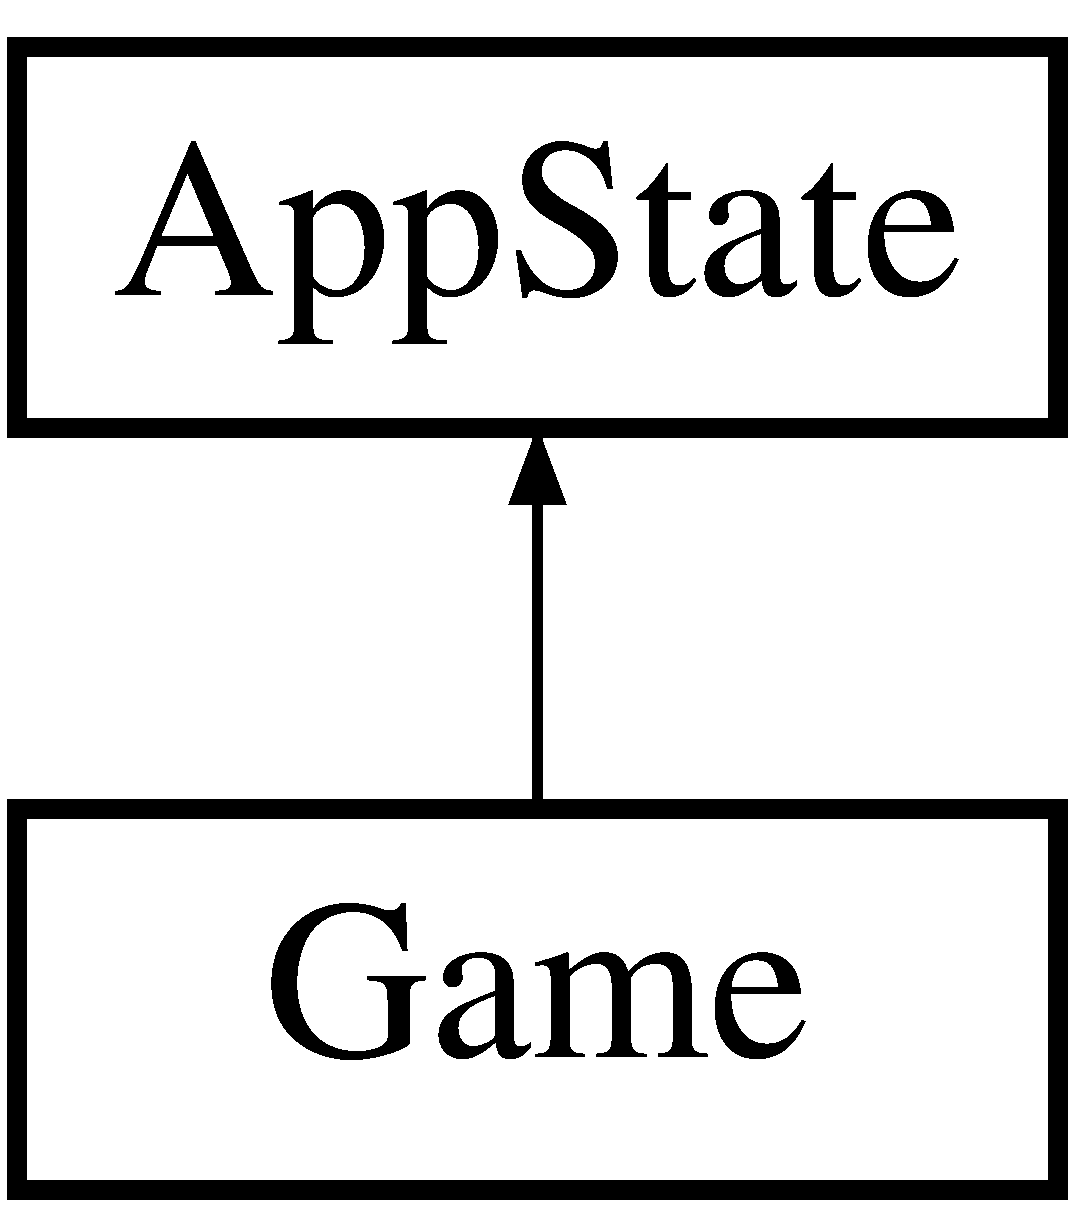
\includegraphics[height=2.000000cm]{class_game}
\end{center}
\end{figure}
\subsection*{Metody publiczne}
\begin{DoxyCompactItemize}
\item 
\hyperlink{class_game_ad59df6562a58a614fda24622d3715b65}{Game} ()
\item 
\hyperlink{class_game_ac39b8dddf91cc448f63ec5dce5783cfd}{Game} (int players\+\_\+count)
\item 
\hyperlink{class_game_a12188b30c73c94a33df229b924c00600}{Game} (std\+::vector$<$ \hyperlink{class_player}{Player} $\ast$ $>$ players, int previous\+\_\+level)
\item 
\hyperlink{class_game_ae3d112ca6e0e55150d2fdbc704474530}{$\sim$\+Game} ()
\item 
bool \hyperlink{class_game_ad425f484c9b48d968ab76632fda9b2f3}{finished} () const 
\item 
void \hyperlink{class_game_a6d54497ce3a66f6dd45eacfdccc8d0bd}{draw} ()
\item 
void \hyperlink{class_game_a502c1be9a7afadbfc679d501034c7b4a}{update} (Uint32 dt)
\item 
void \hyperlink{class_game_abd882b2a5629e55ac4df6d39a6f3311f}{event\+Process} (S\+D\+L\+\_\+\+Event $\ast$ev)
\item 
\hyperlink{class_app_state}{App\+State} $\ast$ \hyperlink{class_game_a7dcc996fd972a30a8038c575a72ccaa2}{next\+State} ()
\end{DoxyCompactItemize}


\subsection{Opis szczegółowy}
Klasa odpowiada za ruch wszytkich czołgów oraz interaakcje między czołgami oraz między czołgami a innymi obiektami na mapie. 

\subsection{Dokumentacja konstruktora i destruktora}
\hypertarget{class_game_ad59df6562a58a614fda24622d3715b65}{}\index{Game@{Game}!Game@{Game}}
\index{Game@{Game}!Game@{Game}}
\subsubsection[{Game}]{\setlength{\rightskip}{0pt plus 5cm}Game\+::\+Game (
\begin{DoxyParamCaption}
{}
\end{DoxyParamCaption}
)}\label{class_game_ad59df6562a58a614fda24622d3715b65}
Domyślny konstruktor -\/ umożliwia grę dla jednego gracza \hypertarget{class_game_ac39b8dddf91cc448f63ec5dce5783cfd}{}\index{Game@{Game}!Game@{Game}}
\index{Game@{Game}!Game@{Game}}
\subsubsection[{Game}]{\setlength{\rightskip}{0pt plus 5cm}Game\+::\+Game (
\begin{DoxyParamCaption}
\item[{int}]{players\+\_\+count}
\end{DoxyParamCaption}
)}\label{class_game_ac39b8dddf91cc448f63ec5dce5783cfd}
Konstruktor pozwalający podać początkową liczbę graczy. Liczba graczy może być równa 1 lub 2, każda inna wartość spowoduje uruchomienie gry dla jednego gracza. Konstruktor jest wywoływany w {\itshape \hyperlink{class_menu_a52b14eefa8e7e9bee6624f759daa5028}{Menu\+::next\+State}}. 
\begin{DoxyParams}{Parametry}
{\em players\+\_\+count} & -\/ liczba graczy 1 lub 2 \\
\hline
\end{DoxyParams}
\hypertarget{class_game_a12188b30c73c94a33df229b924c00600}{}\index{Game@{Game}!Game@{Game}}
\index{Game@{Game}!Game@{Game}}
\subsubsection[{Game}]{\setlength{\rightskip}{0pt plus 5cm}Game\+::\+Game (
\begin{DoxyParamCaption}
\item[{std\+::vector$<$ {\bf Player} $\ast$ $>$}]{players, }
\item[{int}]{previous\+\_\+level}
\end{DoxyParamCaption}
)}\label{class_game_a12188b30c73c94a33df229b924c00600}
Konstruktor przyjmujący już isteniejących graczy. Wywoływany w {\itshape Score\+::next\+State} 
\begin{DoxyParams}{Parametry}
{\em players} & -\/ kontener z graczami \\
\hline
{\em previous\+\_\+level} & -\/ zmienna przechowująca numer poprzedniego poziomu \\
\hline
\end{DoxyParams}
\hypertarget{class_game_ae3d112ca6e0e55150d2fdbc704474530}{}\index{Game@{Game}!````~Game@{$\sim$\+Game}}
\index{````~Game@{$\sim$\+Game}!Game@{Game}}
\subsubsection[{$\sim$\+Game}]{\setlength{\rightskip}{0pt plus 5cm}Game\+::$\sim$\+Game (
\begin{DoxyParamCaption}
{}
\end{DoxyParamCaption}
)}\label{class_game_ae3d112ca6e0e55150d2fdbc704474530}


\subsection{Dokumentacja funkcji składowych}
\hypertarget{class_game_a6d54497ce3a66f6dd45eacfdccc8d0bd}{}\index{Game@{Game}!draw@{draw}}
\index{draw@{draw}!Game@{Game}}
\subsubsection[{draw}]{\setlength{\rightskip}{0pt plus 5cm}void Game\+::draw (
\begin{DoxyParamCaption}
{}
\end{DoxyParamCaption}
)\hspace{0.3cm}{\ttfamily [virtual]}}\label{class_game_a6d54497ce3a66f6dd45eacfdccc8d0bd}
Funkcja wyświetla na początku rundy jej numer. W czasie rozgrywki funkcja odpowiada za rysowanie poziomu (murków, kamieni, wody, lodu, krzewów), graczy, wrogów, bonusów, orzełka, statusu gry na panelu po prawej stronie (pozostałych przeciwników, pozostałe życia graczy, nr rundy). Po przegranej lub podczas pauzy wyświetla odpowiędnią informację na środku ekranu. 

Implementuje \hyperlink{class_app_state_ad2a668dc35b06c330a788e82d9eebee2}{App\+State}.

\hypertarget{class_game_abd882b2a5629e55ac4df6d39a6f3311f}{}\index{Game@{Game}!event\+Process@{event\+Process}}
\index{event\+Process@{event\+Process}!Game@{Game}}
\subsubsection[{event\+Process}]{\setlength{\rightskip}{0pt plus 5cm}void Game\+::event\+Process (
\begin{DoxyParamCaption}
\item[{S\+D\+L\+\_\+\+Event $\ast$}]{ev}
\end{DoxyParamCaption}
)\hspace{0.3cm}{\ttfamily [virtual]}}\label{class_game_abd882b2a5629e55ac4df6d39a6f3311f}
Następuje tu reakcja na klawisze\+: \begin{DoxyItemize}
\item Enter -\/ pauza gry \item Esc -\/ powrót do menu \item n -\/ przejście do następnej rundy, jeśli gra nie jest przegrana \item b -\/ przejście do poprzedniej rundy, jeśli gra nie jest przegrana \item t -\/ pokazanie ścieżek do celów wrogich czołgów 
\begin{DoxyParams}{Parametry}
{\em ev} & -\/ wskaźnik na unię S\+D\+L\+\_\+\+Event przechowującą typ i parametry różnych zdarzeń, w tym zdarzeń klawiatury \\
\hline
\end{DoxyParams}
\end{DoxyItemize}


Implementuje \hyperlink{class_app_state_a9cd9175e5cd251bea2e7eeb4ee9f6137}{App\+State}.

\hypertarget{class_game_ad425f484c9b48d968ab76632fda9b2f3}{}\index{Game@{Game}!finished@{finished}}
\index{finished@{finished}!Game@{Game}}
\subsubsection[{finished}]{\setlength{\rightskip}{0pt plus 5cm}bool Game\+::finished (
\begin{DoxyParamCaption}
{}
\end{DoxyParamCaption}
) const\hspace{0.3cm}{\ttfamily [virtual]}}\label{class_game_ad425f484c9b48d968ab76632fda9b2f3}
Funkcja zwraca {\itshape true} jeśli gracza zniszczył wszystkich przeciwników albo gdy orzełek został trafiony lub gracz stracił wszystkie życia, czyli nastąpiła przegrana. \begin{DoxyReturn}{Zwraca}
{\itshape true} lub {\itshape false} 
\end{DoxyReturn}


Implementuje \hyperlink{class_app_state_ad377464581817ae4000b9cd6c47dc4e8}{App\+State}.

\hypertarget{class_game_a7dcc996fd972a30a8038c575a72ccaa2}{}\index{Game@{Game}!next\+State@{next\+State}}
\index{next\+State@{next\+State}!Game@{Game}}
\subsubsection[{next\+State}]{\setlength{\rightskip}{0pt plus 5cm}{\bf App\+State} $\ast$ Game\+::next\+State (
\begin{DoxyParamCaption}
{}
\end{DoxyParamCaption}
)\hspace{0.3cm}{\ttfamily [virtual]}}\label{class_game_a7dcc996fd972a30a8038c575a72ccaa2}
Przejście do następnyego stanu \begin{DoxyReturn}{Zwraca}
wskaźnik na obiekty klasy {\itshape \hyperlink{class_scores}{Scores}} jeżeli gracz przeszedł rundę lub przegrał. Jeżeli gracz wcisną Esc funkcja zwraca wskaźnik na obiekt {\itshape \hyperlink{class_menu}{Menu}} 
\end{DoxyReturn}


Implementuje \hyperlink{class_app_state_afafba64bbaaf7552f6e0632821c2338f}{App\+State}.

\hypertarget{class_game_a502c1be9a7afadbfc679d501034c7b4a}{}\index{Game@{Game}!update@{update}}
\index{update@{update}!Game@{Game}}
\subsubsection[{update}]{\setlength{\rightskip}{0pt plus 5cm}void Game\+::update (
\begin{DoxyParamCaption}
\item[{Uint32}]{dt}
\end{DoxyParamCaption}
)\hspace{0.3cm}{\ttfamily [virtual]}}\label{class_game_a502c1be9a7afadbfc679d501034c7b4a}
Funkcja aktualizuje stan wszystkich obiektów na planszy (czołgów, bonusów, przeszkód). Sprawdza ponadto kolizje między czołgami, między czołgami i elementami poziomu oraz między pociskami a czołgami i elementami mapy. Naspępuje tu usuwanie zniszczonych obiektów, dodawanie nowych wrogich czołgów oraz sprawdzenie warunków zakończenia rundy. 
\begin{DoxyParams}{Parametry}
{\em dt} & -\/ czas od ostatniego wywołania funkcji w milisekundach \\
\hline
\end{DoxyParams}


Implementuje \hyperlink{class_app_state_a28660de31b5a7a36691b67866f82e5f2}{App\+State}.



Dokumentacja dla tej klasy została wygenerowana z plików\+:\begin{DoxyCompactItemize}
\item 
src/app\+\_\+state/\hyperlink{game_8h}{game.\+h}\item 
src/app\+\_\+state/\hyperlink{game_8cpp}{game.\+cpp}\end{DoxyCompactItemize}

\hypertarget{class_menu}{}\section{Dokumentacja klasy Menu}
\label{class_menu}\index{Menu@{Menu}}


{\ttfamily \#include $<$menu.\+h$>$}

Diagram dziedziczenia dla Menu\begin{figure}[H]
\begin{center}
\leavevmode
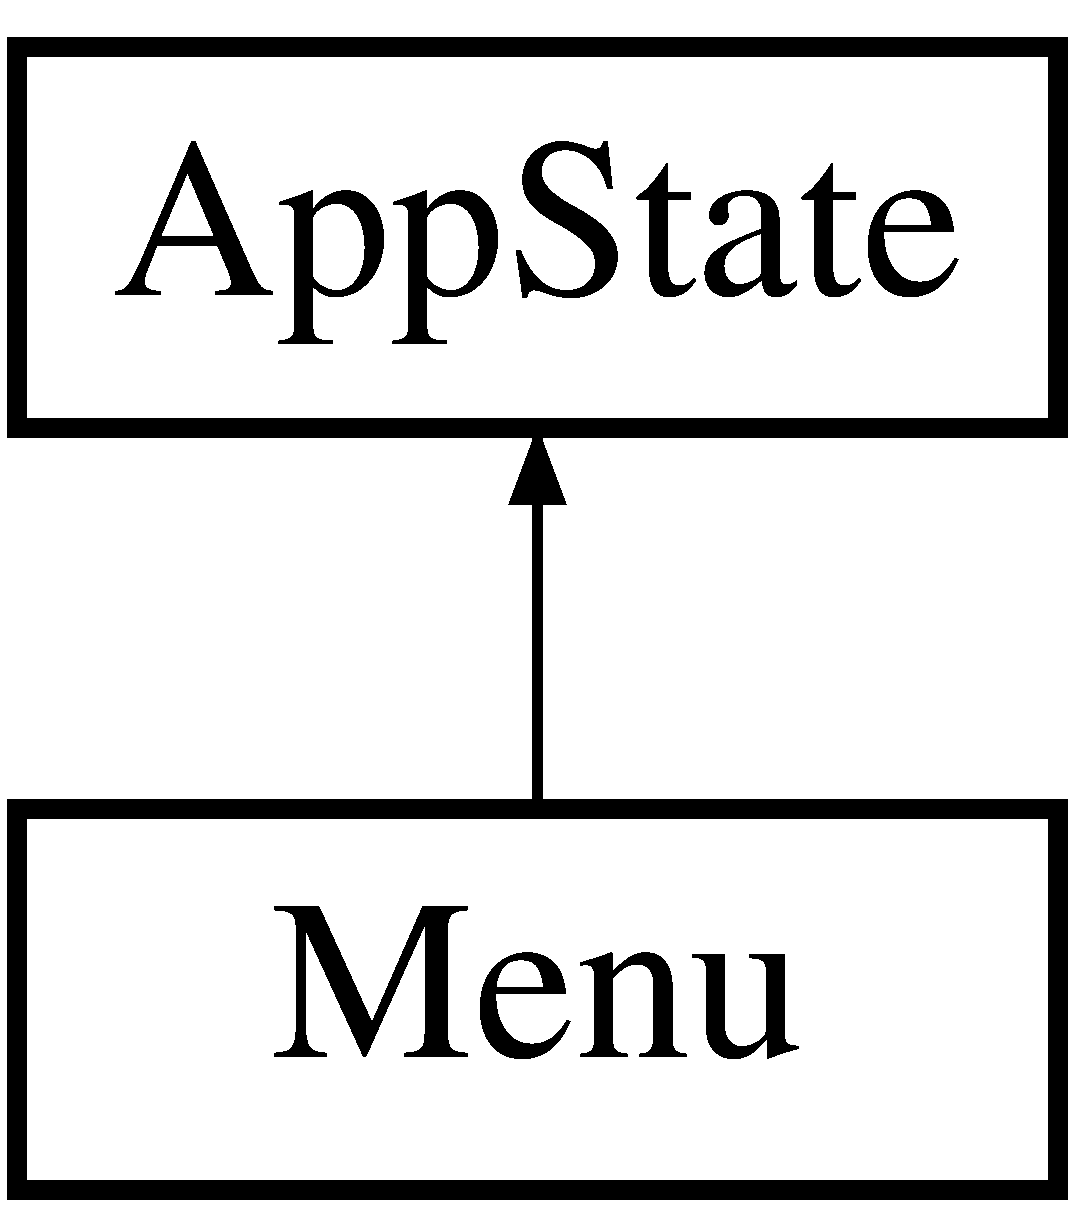
\includegraphics[height=2.000000cm]{class_menu}
\end{center}
\end{figure}
\subsection*{Metody publiczne}
\begin{DoxyCompactItemize}
\item 
\hyperlink{class_menu_ad466dd83355124a6ed958430450bfe94}{Menu} ()
\item 
\hyperlink{class_menu_a831387f51358cfb88cd018e1777bc980}{$\sim$\+Menu} ()
\item 
bool \hyperlink{class_menu_ac72d49b5565464340c2c25bd335c9424}{finished} () const 
\item 
void \hyperlink{class_menu_a2cd7ab9901a8f42a3ae977d0774398a6}{draw} ()
\item 
void \hyperlink{class_menu_a02ff964c4a203ca08b11655c36252fc8}{update} (Uint32 dt)
\item 
void \hyperlink{class_menu_a0b84052947f8687e10afe15ec88c90a9}{event\+Process} (S\+D\+L\+\_\+\+Event $\ast$ev)
\item 
\hyperlink{class_app_state}{App\+State} $\ast$ \hyperlink{class_menu_a52b14eefa8e7e9bee6624f759daa5028}{next\+State} ()
\end{DoxyCompactItemize}


\subsection{Dokumentacja konstruktora i destruktora}
\hypertarget{class_menu_ad466dd83355124a6ed958430450bfe94}{}\index{Menu@{Menu}!Menu@{Menu}}
\index{Menu@{Menu}!Menu@{Menu}}
\subsubsection[{Menu}]{\setlength{\rightskip}{0pt plus 5cm}Menu\+::\+Menu (
\begin{DoxyParamCaption}
{}
\end{DoxyParamCaption}
)}\label{class_menu_ad466dd83355124a6ed958430450bfe94}
\hypertarget{class_menu_a831387f51358cfb88cd018e1777bc980}{}\index{Menu@{Menu}!````~Menu@{$\sim$\+Menu}}
\index{````~Menu@{$\sim$\+Menu}!Menu@{Menu}}
\subsubsection[{$\sim$\+Menu}]{\setlength{\rightskip}{0pt plus 5cm}Menu\+::$\sim$\+Menu (
\begin{DoxyParamCaption}
{}
\end{DoxyParamCaption}
)}\label{class_menu_a831387f51358cfb88cd018e1777bc980}


\subsection{Dokumentacja funkcji składowych}
\hypertarget{class_menu_a2cd7ab9901a8f42a3ae977d0774398a6}{}\index{Menu@{Menu}!draw@{draw}}
\index{draw@{draw}!Menu@{Menu}}
\subsubsection[{draw}]{\setlength{\rightskip}{0pt plus 5cm}void Menu\+::draw (
\begin{DoxyParamCaption}
{}
\end{DoxyParamCaption}
)\hspace{0.3cm}{\ttfamily [virtual]}}\label{class_menu_a2cd7ab9901a8f42a3ae977d0774398a6}
Funkcja rysująca elementy gry należące do danego stanu 

Implementuje \hyperlink{class_app_state_ad2a668dc35b06c330a788e82d9eebee2}{App\+State}.

\hypertarget{class_menu_a0b84052947f8687e10afe15ec88c90a9}{}\index{Menu@{Menu}!event\+Process@{event\+Process}}
\index{event\+Process@{event\+Process}!Menu@{Menu}}
\subsubsection[{event\+Process}]{\setlength{\rightskip}{0pt plus 5cm}void Menu\+::event\+Process (
\begin{DoxyParamCaption}
\item[{S\+D\+L\+\_\+\+Event $\ast$}]{ev}
\end{DoxyParamCaption}
)\hspace{0.3cm}{\ttfamily [virtual]}}\label{class_menu_a0b84052947f8687e10afe15ec88c90a9}
Funkcja umożliwiająca obsługę zdarzeń wykrywanych przez bibliotekę S\+D\+L2. 
\begin{DoxyParams}{Parametry}
{\em ev} & -\/ wskaźnik na unię S\+D\+L\+\_\+\+Event przechowującą typ i parametry różnych zdarzeń \\
\hline
\end{DoxyParams}


Implementuje \hyperlink{class_app_state_a9cd9175e5cd251bea2e7eeb4ee9f6137}{App\+State}.

\hypertarget{class_menu_ac72d49b5565464340c2c25bd335c9424}{}\index{Menu@{Menu}!finished@{finished}}
\index{finished@{finished}!Menu@{Menu}}
\subsubsection[{finished}]{\setlength{\rightskip}{0pt plus 5cm}bool Menu\+::finished (
\begin{DoxyParamCaption}
{}
\end{DoxyParamCaption}
) const\hspace{0.3cm}{\ttfamily [virtual]}}\label{class_menu_ac72d49b5565464340c2c25bd335c9424}
Funkcja sprawdza czy aktualny stan gry się skończył. \begin{DoxyReturn}{Zwraca}
{\itshape true} jeżeli obecny stan gry się skończył, w przeciwnym wypadku {\itshape false}. 
\end{DoxyReturn}


Implementuje \hyperlink{class_app_state_ad377464581817ae4000b9cd6c47dc4e8}{App\+State}.

\hypertarget{class_menu_a52b14eefa8e7e9bee6624f759daa5028}{}\index{Menu@{Menu}!next\+State@{next\+State}}
\index{next\+State@{next\+State}!Menu@{Menu}}
\subsubsection[{next\+State}]{\setlength{\rightskip}{0pt plus 5cm}{\bf App\+State} $\ast$ Menu\+::next\+State (
\begin{DoxyParamCaption}
{}
\end{DoxyParamCaption}
)\hspace{0.3cm}{\ttfamily [virtual]}}\label{class_menu_a52b14eefa8e7e9bee6624f759daa5028}
Funkcja zwracającya następny stan po zakończeniu obecnego. Funkcję należy wywołać tylko wtedy, gdy funkcja {\itshape finished} zwróci wartość 1. \begin{DoxyReturn}{Zwraca}
następny stan gry 
\end{DoxyReturn}


Implementuje \hyperlink{class_app_state_afafba64bbaaf7552f6e0632821c2338f}{App\+State}.

\hypertarget{class_menu_a02ff964c4a203ca08b11655c36252fc8}{}\index{Menu@{Menu}!update@{update}}
\index{update@{update}!Menu@{Menu}}
\subsubsection[{update}]{\setlength{\rightskip}{0pt plus 5cm}void Menu\+::update (
\begin{DoxyParamCaption}
\item[{Uint32}]{dt}
\end{DoxyParamCaption}
)\hspace{0.3cm}{\ttfamily [virtual]}}\label{class_menu_a02ff964c4a203ca08b11655c36252fc8}
Funkcja aktualizująca stan obiektów i liczników w grze 
\begin{DoxyParams}{Parametry}
{\em dt} & -\/ czas od ostatniego wywołania funkcji w milisekundach \\
\hline
\end{DoxyParams}


Implementuje \hyperlink{class_app_state_a28660de31b5a7a36691b67866f82e5f2}{App\+State}.



Dokumentacja dla tej klasy została wygenerowana z plików\+:\begin{DoxyCompactItemize}
\item 
src/app\+\_\+state/\hyperlink{menu_8h}{menu.\+h}\item 
src/app\+\_\+state/\hyperlink{menu_8cpp}{menu.\+cpp}\end{DoxyCompactItemize}

\hypertarget{class_object}{}\section{Dokumentacja klasy Object}
\label{class_object}\index{Object@{Object}}


{\ttfamily \#include $<$object.\+h$>$}

Diagram dziedziczenia dla Object\begin{figure}[H]
\begin{center}
\leavevmode
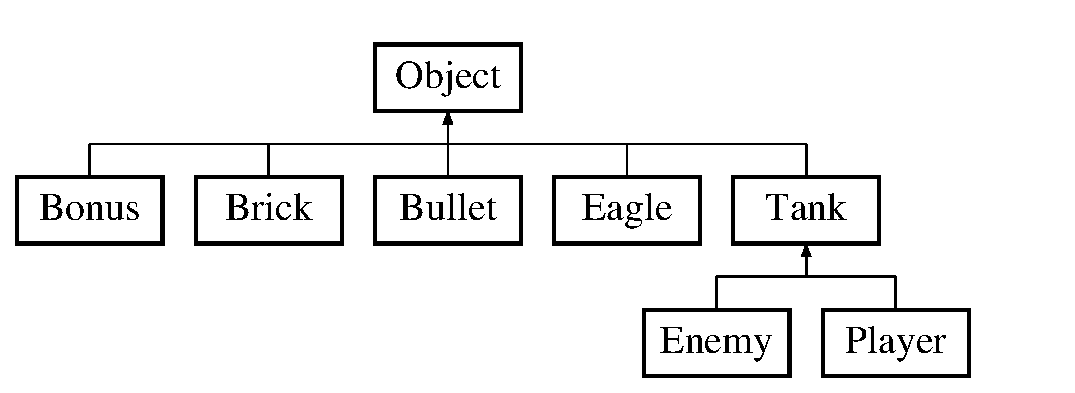
\includegraphics[height=3.000000cm]{class_object}
\end{center}
\end{figure}
\subsection*{Metody publiczne}
\begin{DoxyCompactItemize}
\item 
\hyperlink{class_object_a40860402e64d8008fb42329df7097cdb}{Object} ()
\item 
\hyperlink{class_object_aaf2083b10a26fc519b5a2bb79aaf6986}{Object} (double x, double y, \hyperlink{type_8h_ac6fa10729dffeb6a192492f13c25e31a}{Sprite\+Type} \hyperlink{class_object_a1b89f32cd9e0040f8a2455f3cef7d0d2}{type})
\item 
\hyperlink{class_object_a8738ecc2b99c528875cf98787ceff25b}{Object} (double x, double y, const \hyperlink{struct_sprite_data}{Sprite\+Data} $\ast$sprite)
\item 
virtual \hyperlink{class_object_ae8f5483f459e46687bd01e6f9977afd3}{$\sim$\+Object} ()
\item 
virtual void \hyperlink{class_object_a821f5b25b450fa1acdb3f9c0b5962592}{draw} ()
\item 
virtual void \hyperlink{class_object_a02c1621329cb9ec5268072a2402d2ac5}{update} (Uint32 dt)
\end{DoxyCompactItemize}
\subsection*{Atrybuty publiczne}
\begin{DoxyCompactItemize}
\item 
bool \hyperlink{class_object_a77c2ada7189758c530ab24a7b366d3fb}{to\+\_\+erase}
\item 
S\+D\+L\+\_\+\+Rect \hyperlink{class_object_a308c5fde145e854d4a2808283f18e14b}{collision\+\_\+rect}
\item 
S\+D\+L\+\_\+\+Rect \hyperlink{class_object_aa11a2e0ccb927f542aee786bc7bd731d}{dest\+\_\+rect}
\item 
S\+D\+L\+\_\+\+Rect \hyperlink{class_object_aef9bec0e47c5d8cc04145de236881f47}{src\+\_\+rect}
\item 
\hyperlink{type_8h_ac6fa10729dffeb6a192492f13c25e31a}{Sprite\+Type} \hyperlink{class_object_a1b89f32cd9e0040f8a2455f3cef7d0d2}{type}
\item 
double \hyperlink{class_object_a1f71a5693147aecc701db4ab51d3edcc}{pos\+\_\+x}
\item 
double \hyperlink{class_object_a986134c27f3e74ba41a4d28e20b183a9}{pos\+\_\+y}
\end{DoxyCompactItemize}
\subsection*{Metody chronione}
\begin{DoxyCompactItemize}
\item 
S\+D\+L\+\_\+\+Rect \hyperlink{class_object_a98ac32f03f7ec5f9bf082cd697a9b4fc}{move\+Rect} (const S\+D\+L\+\_\+\+Rect \&rect, int x, int y)
\end{DoxyCompactItemize}
\subsection*{Atrybuty chronione}
\begin{DoxyCompactItemize}
\item 
const \hyperlink{struct_sprite_data}{Sprite\+Data} $\ast$ \hyperlink{class_object_a07c5c7138bb081dacbe9ddfb0295ced7}{m\+\_\+sprite}
\item 
Uint32 \hyperlink{class_object_a76a3f8ee17746de53b8f162b5df2c837}{m\+\_\+frame\+\_\+display\+\_\+time}
\item 
int \hyperlink{class_object_a4e03c944bc9142a5c34b7049c20c4301}{m\+\_\+current\+\_\+frame}
\end{DoxyCompactItemize}


\subsection{Dokumentacja konstruktora i destruktora}
\hypertarget{class_object_a40860402e64d8008fb42329df7097cdb}{}\index{Object@{Object}!Object@{Object}}
\index{Object@{Object}!Object@{Object}}
\subsubsection[{Object}]{\setlength{\rightskip}{0pt plus 5cm}Object\+::\+Object (
\begin{DoxyParamCaption}
{}
\end{DoxyParamCaption}
)}\label{class_object_a40860402e64d8008fb42329df7097cdb}
\hypertarget{class_object_aaf2083b10a26fc519b5a2bb79aaf6986}{}\index{Object@{Object}!Object@{Object}}
\index{Object@{Object}!Object@{Object}}
\subsubsection[{Object}]{\setlength{\rightskip}{0pt plus 5cm}Object\+::\+Object (
\begin{DoxyParamCaption}
\item[{double}]{x, }
\item[{double}]{y, }
\item[{{\bf Sprite\+Type}}]{type}
\end{DoxyParamCaption}
)}\label{class_object_aaf2083b10a26fc519b5a2bb79aaf6986}
\hypertarget{class_object_a8738ecc2b99c528875cf98787ceff25b}{}\index{Object@{Object}!Object@{Object}}
\index{Object@{Object}!Object@{Object}}
\subsubsection[{Object}]{\setlength{\rightskip}{0pt plus 5cm}Object\+::\+Object (
\begin{DoxyParamCaption}
\item[{double}]{x, }
\item[{double}]{y, }
\item[{const {\bf Sprite\+Data} $\ast$}]{sprite}
\end{DoxyParamCaption}
)}\label{class_object_a8738ecc2b99c528875cf98787ceff25b}
\hypertarget{class_object_ae8f5483f459e46687bd01e6f9977afd3}{}\index{Object@{Object}!````~Object@{$\sim$\+Object}}
\index{````~Object@{$\sim$\+Object}!Object@{Object}}
\subsubsection[{$\sim$\+Object}]{\setlength{\rightskip}{0pt plus 5cm}Object\+::$\sim$\+Object (
\begin{DoxyParamCaption}
{}
\end{DoxyParamCaption}
)\hspace{0.3cm}{\ttfamily [virtual]}}\label{class_object_ae8f5483f459e46687bd01e6f9977afd3}


\subsection{Dokumentacja funkcji składowych}
\hypertarget{class_object_a821f5b25b450fa1acdb3f9c0b5962592}{}\index{Object@{Object}!draw@{draw}}
\index{draw@{draw}!Object@{Object}}
\subsubsection[{draw}]{\setlength{\rightskip}{0pt plus 5cm}void Object\+::draw (
\begin{DoxyParamCaption}
{}
\end{DoxyParamCaption}
)\hspace{0.3cm}{\ttfamily [virtual]}}\label{class_object_a821f5b25b450fa1acdb3f9c0b5962592}


Reimplementowana w \hyperlink{class_tank_ab30c54bb7378b522fa965d4e8ab7ed4f}{Tank}, \hyperlink{class_bonus_a00a6ad75da471b6a577029be0b80e259}{Bonus} i \hyperlink{class_enemy_a7dcf45915f6288ef9264ec60af621b6c}{Enemy}.

\hypertarget{class_object_a98ac32f03f7ec5f9bf082cd697a9b4fc}{}\index{Object@{Object}!move\+Rect@{move\+Rect}}
\index{move\+Rect@{move\+Rect}!Object@{Object}}
\subsubsection[{move\+Rect}]{\setlength{\rightskip}{0pt plus 5cm}S\+D\+L\+\_\+\+Rect Object\+::move\+Rect (
\begin{DoxyParamCaption}
\item[{const S\+D\+L\+\_\+\+Rect \&}]{rect, }
\item[{int}]{x, }
\item[{int}]{y}
\end{DoxyParamCaption}
)\hspace{0.3cm}{\ttfamily [protected]}}\label{class_object_a98ac32f03f7ec5f9bf082cd697a9b4fc}
\hypertarget{class_object_a02c1621329cb9ec5268072a2402d2ac5}{}\index{Object@{Object}!update@{update}}
\index{update@{update}!Object@{Object}}
\subsubsection[{update}]{\setlength{\rightskip}{0pt plus 5cm}void Object\+::update (
\begin{DoxyParamCaption}
\item[{Uint32}]{dt}
\end{DoxyParamCaption}
)\hspace{0.3cm}{\ttfamily [virtual]}}\label{class_object_a02c1621329cb9ec5268072a2402d2ac5}


Reimplementowana w \hyperlink{class_player_af5cac4f8c62903d39c7dc7bdf8f05ddb}{Player}, \hyperlink{class_tank_a1278dfec0f2d1d3bb1f4ce0a19957c0f}{Tank}, \hyperlink{class_bonus_a53c7235c0dae0deddfc95a2b7c5a594b}{Bonus}, \hyperlink{class_enemy_a03c09cab6c4950e4cae880c15b2fd739}{Enemy}, \hyperlink{class_brick_a31098851b4f1224cfd6b51c4ef47094f}{Brick}, \hyperlink{class_bullet_a28c27c103a23f73d18125791c973cccd}{Bullet} i \hyperlink{class_eagle_a609e173a641783b14973d5e1055f192a}{Eagle}.



\subsection{Dokumentacja atrybutów składowych}
\hypertarget{class_object_a308c5fde145e854d4a2808283f18e14b}{}\index{Object@{Object}!collision\+\_\+rect@{collision\+\_\+rect}}
\index{collision\+\_\+rect@{collision\+\_\+rect}!Object@{Object}}
\subsubsection[{collision\+\_\+rect}]{\setlength{\rightskip}{0pt plus 5cm}S\+D\+L\+\_\+\+Rect Object\+::collision\+\_\+rect}\label{class_object_a308c5fde145e854d4a2808283f18e14b}
\hypertarget{class_object_aa11a2e0ccb927f542aee786bc7bd731d}{}\index{Object@{Object}!dest\+\_\+rect@{dest\+\_\+rect}}
\index{dest\+\_\+rect@{dest\+\_\+rect}!Object@{Object}}
\subsubsection[{dest\+\_\+rect}]{\setlength{\rightskip}{0pt plus 5cm}S\+D\+L\+\_\+\+Rect Object\+::dest\+\_\+rect}\label{class_object_aa11a2e0ccb927f542aee786bc7bd731d}
\hypertarget{class_object_a4e03c944bc9142a5c34b7049c20c4301}{}\index{Object@{Object}!m\+\_\+current\+\_\+frame@{m\+\_\+current\+\_\+frame}}
\index{m\+\_\+current\+\_\+frame@{m\+\_\+current\+\_\+frame}!Object@{Object}}
\subsubsection[{m\+\_\+current\+\_\+frame}]{\setlength{\rightskip}{0pt plus 5cm}int Object\+::m\+\_\+current\+\_\+frame\hspace{0.3cm}{\ttfamily [protected]}}\label{class_object_a4e03c944bc9142a5c34b7049c20c4301}
\hypertarget{class_object_a76a3f8ee17746de53b8f162b5df2c837}{}\index{Object@{Object}!m\+\_\+frame\+\_\+display\+\_\+time@{m\+\_\+frame\+\_\+display\+\_\+time}}
\index{m\+\_\+frame\+\_\+display\+\_\+time@{m\+\_\+frame\+\_\+display\+\_\+time}!Object@{Object}}
\subsubsection[{m\+\_\+frame\+\_\+display\+\_\+time}]{\setlength{\rightskip}{0pt plus 5cm}Uint32 Object\+::m\+\_\+frame\+\_\+display\+\_\+time\hspace{0.3cm}{\ttfamily [protected]}}\label{class_object_a76a3f8ee17746de53b8f162b5df2c837}
\hypertarget{class_object_a07c5c7138bb081dacbe9ddfb0295ced7}{}\index{Object@{Object}!m\+\_\+sprite@{m\+\_\+sprite}}
\index{m\+\_\+sprite@{m\+\_\+sprite}!Object@{Object}}
\subsubsection[{m\+\_\+sprite}]{\setlength{\rightskip}{0pt plus 5cm}const {\bf Sprite\+Data}$\ast$ Object\+::m\+\_\+sprite\hspace{0.3cm}{\ttfamily [protected]}}\label{class_object_a07c5c7138bb081dacbe9ddfb0295ced7}
\hypertarget{class_object_a1f71a5693147aecc701db4ab51d3edcc}{}\index{Object@{Object}!pos\+\_\+x@{pos\+\_\+x}}
\index{pos\+\_\+x@{pos\+\_\+x}!Object@{Object}}
\subsubsection[{pos\+\_\+x}]{\setlength{\rightskip}{0pt plus 5cm}double Object\+::pos\+\_\+x}\label{class_object_a1f71a5693147aecc701db4ab51d3edcc}
\hypertarget{class_object_a986134c27f3e74ba41a4d28e20b183a9}{}\index{Object@{Object}!pos\+\_\+y@{pos\+\_\+y}}
\index{pos\+\_\+y@{pos\+\_\+y}!Object@{Object}}
\subsubsection[{pos\+\_\+y}]{\setlength{\rightskip}{0pt plus 5cm}double Object\+::pos\+\_\+y}\label{class_object_a986134c27f3e74ba41a4d28e20b183a9}
\hypertarget{class_object_aef9bec0e47c5d8cc04145de236881f47}{}\index{Object@{Object}!src\+\_\+rect@{src\+\_\+rect}}
\index{src\+\_\+rect@{src\+\_\+rect}!Object@{Object}}
\subsubsection[{src\+\_\+rect}]{\setlength{\rightskip}{0pt plus 5cm}S\+D\+L\+\_\+\+Rect Object\+::src\+\_\+rect}\label{class_object_aef9bec0e47c5d8cc04145de236881f47}
\hypertarget{class_object_a77c2ada7189758c530ab24a7b366d3fb}{}\index{Object@{Object}!to\+\_\+erase@{to\+\_\+erase}}
\index{to\+\_\+erase@{to\+\_\+erase}!Object@{Object}}
\subsubsection[{to\+\_\+erase}]{\setlength{\rightskip}{0pt plus 5cm}bool Object\+::to\+\_\+erase}\label{class_object_a77c2ada7189758c530ab24a7b366d3fb}
\hypertarget{class_object_a1b89f32cd9e0040f8a2455f3cef7d0d2}{}\index{Object@{Object}!type@{type}}
\index{type@{type}!Object@{Object}}
\subsubsection[{type}]{\setlength{\rightskip}{0pt plus 5cm}{\bf Sprite\+Type} Object\+::type}\label{class_object_a1b89f32cd9e0040f8a2455f3cef7d0d2}


Dokumentacja dla tej klasy została wygenerowana z plików\+:\begin{DoxyCompactItemize}
\item 
src/objects/\hyperlink{object_8h}{object.\+h}\item 
src/objects/\hyperlink{object_8cpp}{object.\+cpp}\end{DoxyCompactItemize}

\hypertarget{class_player}{}\section{Dokumentacja klasy Player}
\label{class_player}\index{Player@{Player}}


{\ttfamily \#include $<$player.\+h$>$}

Diagram dziedziczenia dla Player\begin{figure}[H]
\begin{center}
\leavevmode
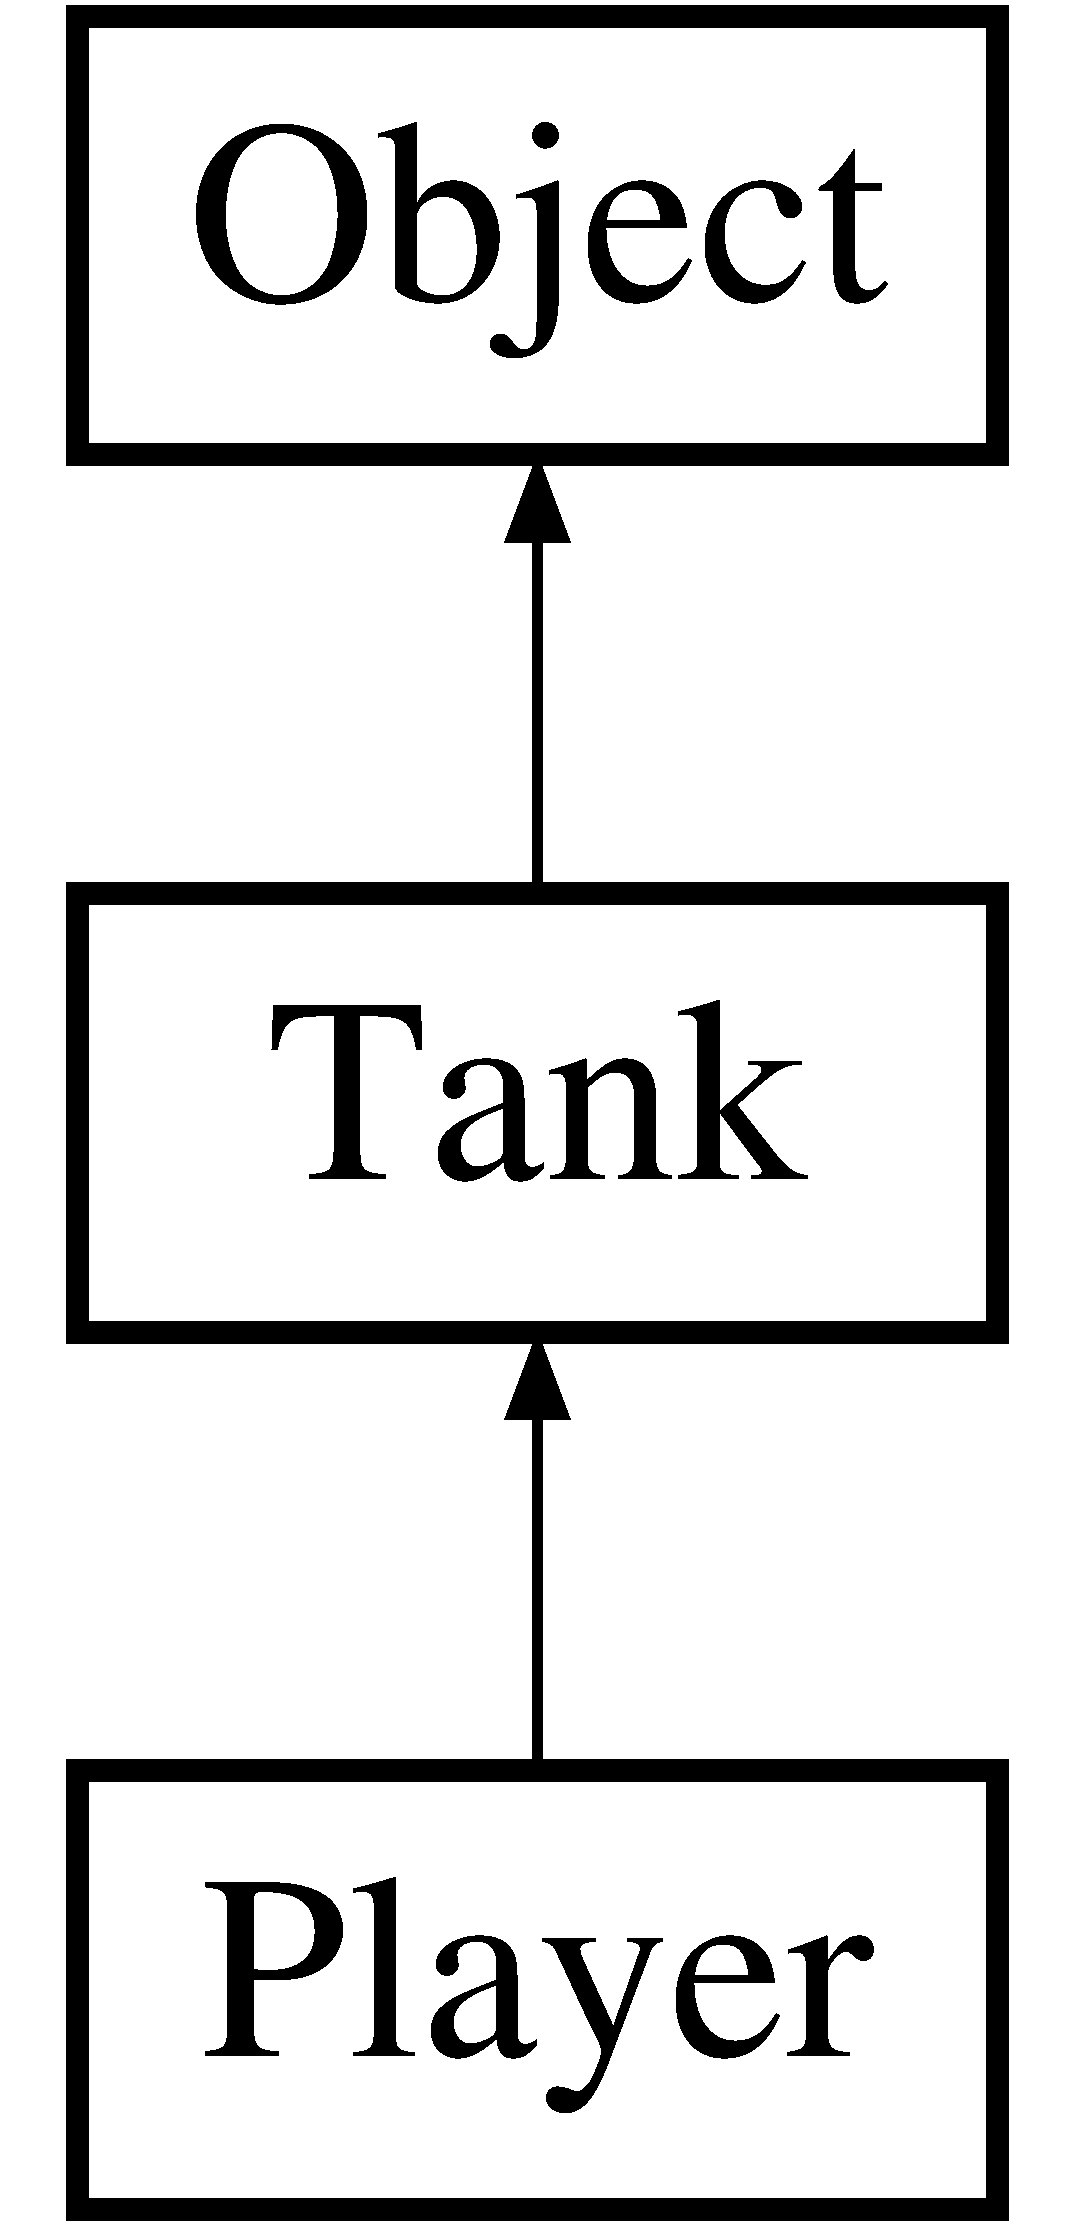
\includegraphics[height=3.000000cm]{class_player}
\end{center}
\end{figure}
\subsection*{Komponenty}
\begin{DoxyCompactItemize}
\item 
struct \hyperlink{struct_player_1_1_player_keys}{Player\+Keys}
\end{DoxyCompactItemize}
\subsection*{Metody publiczne}
\begin{DoxyCompactItemize}
\item 
\hyperlink{class_player_affe0cc3cb714f6deb4e62f0c0d3f1fd8}{Player} ()
\item 
\hyperlink{class_player_abea91b1e21cd330be03345417b9e6f2d}{Player} (double x, double y, \hyperlink{type_8h_ac6fa10729dffeb6a192492f13c25e31a}{Sprite\+Type} \hyperlink{class_object_a1b89f32cd9e0040f8a2455f3cef7d0d2}{type})
\item 
void \hyperlink{class_player_af5cac4f8c62903d39c7dc7bdf8f05ddb}{update} (Uint32 dt)
\item 
void \hyperlink{class_player_a038a74bd768b6eec8fbe57cb2bacf811}{respawn} ()
\item 
void \hyperlink{class_player_acb40d0a5d388029d48156fb06fdd288c}{destroy} ()
\item 
\hyperlink{class_bullet}{Bullet} $\ast$ \hyperlink{class_player_a5f0f389fdf5d685f088a997ed5af925d}{fire} ()
\item 
void \hyperlink{class_player_aa7495c2cb4ba4f197f0d6228970de75b}{change\+Star\+Count\+By} (int c)
\end{DoxyCompactItemize}
\subsection*{Atrybuty publiczne}
\begin{DoxyCompactItemize}
\item 
\hyperlink{struct_player_1_1_player_keys}{Player\+Keys} \hyperlink{class_player_a9822b1b86085cc46c773c76570cfaa4d}{player\+\_\+keys}
\item 
unsigned \hyperlink{class_player_a18afa2dfc1f6dfba7bbe08889f443da5}{score}
\item 
int \hyperlink{class_player_a331b0f5de5a558249b8a14441249279b}{star\+\_\+count}
\end{DoxyCompactItemize}
\subsection*{Dodatkowe Dziedziczone Składowe}


\subsection{Dokumentacja konstruktora i destruktora}
\hypertarget{class_player_affe0cc3cb714f6deb4e62f0c0d3f1fd8}{}\index{Player@{Player}!Player@{Player}}
\index{Player@{Player}!Player@{Player}}
\subsubsection[{Player}]{\setlength{\rightskip}{0pt plus 5cm}Player\+::\+Player (
\begin{DoxyParamCaption}
{}
\end{DoxyParamCaption}
)}\label{class_player_affe0cc3cb714f6deb4e62f0c0d3f1fd8}
\hypertarget{class_player_abea91b1e21cd330be03345417b9e6f2d}{}\index{Player@{Player}!Player@{Player}}
\index{Player@{Player}!Player@{Player}}
\subsubsection[{Player}]{\setlength{\rightskip}{0pt plus 5cm}Player\+::\+Player (
\begin{DoxyParamCaption}
\item[{double}]{x, }
\item[{double}]{y, }
\item[{{\bf Sprite\+Type}}]{type}
\end{DoxyParamCaption}
)}\label{class_player_abea91b1e21cd330be03345417b9e6f2d}


\subsection{Dokumentacja funkcji składowych}
\hypertarget{class_player_aa7495c2cb4ba4f197f0d6228970de75b}{}\index{Player@{Player}!change\+Star\+Count\+By@{change\+Star\+Count\+By}}
\index{change\+Star\+Count\+By@{change\+Star\+Count\+By}!Player@{Player}}
\subsubsection[{change\+Star\+Count\+By}]{\setlength{\rightskip}{0pt plus 5cm}void Player\+::change\+Star\+Count\+By (
\begin{DoxyParamCaption}
\item[{int}]{c}
\end{DoxyParamCaption}
)}\label{class_player_aa7495c2cb4ba4f197f0d6228970de75b}
\hypertarget{class_player_acb40d0a5d388029d48156fb06fdd288c}{}\index{Player@{Player}!destroy@{destroy}}
\index{destroy@{destroy}!Player@{Player}}
\subsubsection[{destroy}]{\setlength{\rightskip}{0pt plus 5cm}void Player\+::destroy (
\begin{DoxyParamCaption}
{}
\end{DoxyParamCaption}
)\hspace{0.3cm}{\ttfamily [virtual]}}\label{class_player_acb40d0a5d388029d48156fb06fdd288c}


Reimplementowana z \hyperlink{class_tank_a5d2e3302417166ccdc42b8bc2e5d5dc4}{Tank}.

\hypertarget{class_player_a5f0f389fdf5d685f088a997ed5af925d}{}\index{Player@{Player}!fire@{fire}}
\index{fire@{fire}!Player@{Player}}
\subsubsection[{fire}]{\setlength{\rightskip}{0pt plus 5cm}{\bf Bullet} $\ast$ Player\+::fire (
\begin{DoxyParamCaption}
{}
\end{DoxyParamCaption}
)\hspace{0.3cm}{\ttfamily [virtual]}}\label{class_player_a5f0f389fdf5d685f088a997ed5af925d}


Reimplementowana z \hyperlink{class_tank_ae5c683a77507d638b2e2d7526e5205de}{Tank}.

\hypertarget{class_player_a038a74bd768b6eec8fbe57cb2bacf811}{}\index{Player@{Player}!respawn@{respawn}}
\index{respawn@{respawn}!Player@{Player}}
\subsubsection[{respawn}]{\setlength{\rightskip}{0pt plus 5cm}void Player\+::respawn (
\begin{DoxyParamCaption}
{}
\end{DoxyParamCaption}
)\hspace{0.3cm}{\ttfamily [virtual]}}\label{class_player_a038a74bd768b6eec8fbe57cb2bacf811}


Reimplementowana z \hyperlink{class_tank_a61501e1b99fd235500b79f39c6b2fc8f}{Tank}.

\hypertarget{class_player_af5cac4f8c62903d39c7dc7bdf8f05ddb}{}\index{Player@{Player}!update@{update}}
\index{update@{update}!Player@{Player}}
\subsubsection[{update}]{\setlength{\rightskip}{0pt plus 5cm}void Player\+::update (
\begin{DoxyParamCaption}
\item[{Uint32}]{dt}
\end{DoxyParamCaption}
)\hspace{0.3cm}{\ttfamily [virtual]}}\label{class_player_af5cac4f8c62903d39c7dc7bdf8f05ddb}


Reimplementowana z \hyperlink{class_object_a02c1621329cb9ec5268072a2402d2ac5}{Object}.



\subsection{Dokumentacja atrybutów składowych}
\hypertarget{class_player_a9822b1b86085cc46c773c76570cfaa4d}{}\index{Player@{Player}!player\+\_\+keys@{player\+\_\+keys}}
\index{player\+\_\+keys@{player\+\_\+keys}!Player@{Player}}
\subsubsection[{player\+\_\+keys}]{\setlength{\rightskip}{0pt plus 5cm}{\bf Player\+Keys} Player\+::player\+\_\+keys}\label{class_player_a9822b1b86085cc46c773c76570cfaa4d}
\hypertarget{class_player_a18afa2dfc1f6dfba7bbe08889f443da5}{}\index{Player@{Player}!score@{score}}
\index{score@{score}!Player@{Player}}
\subsubsection[{score}]{\setlength{\rightskip}{0pt plus 5cm}unsigned Player\+::score}\label{class_player_a18afa2dfc1f6dfba7bbe08889f443da5}
\hypertarget{class_player_a331b0f5de5a558249b8a14441249279b}{}\index{Player@{Player}!star\+\_\+count@{star\+\_\+count}}
\index{star\+\_\+count@{star\+\_\+count}!Player@{Player}}
\subsubsection[{star\+\_\+count}]{\setlength{\rightskip}{0pt plus 5cm}int Player\+::star\+\_\+count}\label{class_player_a331b0f5de5a558249b8a14441249279b}


Dokumentacja dla tej klasy została wygenerowana z plików\+:\begin{DoxyCompactItemize}
\item 
src/objects/\hyperlink{player_8h}{player.\+h}\item 
src/objects/\hyperlink{player_8cpp}{player.\+cpp}\end{DoxyCompactItemize}

\hypertarget{struct_player_1_1_player_keys}{}\section{Dokumentacja struktury Player\+:\+:Player\+Keys}
\label{struct_player_1_1_player_keys}\index{Player\+::\+Player\+Keys@{Player\+::\+Player\+Keys}}


{\ttfamily \#include $<$player.\+h$>$}

\subsection*{Metody publiczne}
\begin{DoxyCompactItemize}
\item 
\hyperlink{struct_player_1_1_player_keys_a56a56f4201c50a48bb847971c94ca4b1}{Player\+Keys} ()
\item 
\hyperlink{struct_player_1_1_player_keys_abfa5fbc24fae22b69a060b7ce5812aab}{Player\+Keys} (S\+D\+L\+\_\+\+Scancode u, S\+D\+L\+\_\+\+Scancode d, S\+D\+L\+\_\+\+Scancode l, S\+D\+L\+\_\+\+Scancode r, S\+D\+L\+\_\+\+Scancode f)
\end{DoxyCompactItemize}
\subsection*{Atrybuty publiczne}
\begin{DoxyCompactItemize}
\item 
S\+D\+L\+\_\+\+Scancode \hyperlink{struct_player_1_1_player_keys_a943bcfbd15d886d3d2a397343717dd4f}{up}
\item 
S\+D\+L\+\_\+\+Scancode \hyperlink{struct_player_1_1_player_keys_a57aab79d509ab35da6ee806f92299679}{down}
\item 
S\+D\+L\+\_\+\+Scancode \hyperlink{struct_player_1_1_player_keys_a963bc2b65a3e864cb863a0ed5d77a233}{left}
\item 
S\+D\+L\+\_\+\+Scancode \hyperlink{struct_player_1_1_player_keys_a0ed2777f9a657033b9ceb04302fea7c5}{right}
\item 
S\+D\+L\+\_\+\+Scancode \hyperlink{struct_player_1_1_player_keys_ae9a752c12df2b347234bb7acefe93ed0}{fire}
\end{DoxyCompactItemize}


\subsection{Dokumentacja konstruktora i destruktora}
\hypertarget{struct_player_1_1_player_keys_a56a56f4201c50a48bb847971c94ca4b1}{}\index{Player\+::\+Player\+Keys@{Player\+::\+Player\+Keys}!Player\+Keys@{Player\+Keys}}
\index{Player\+Keys@{Player\+Keys}!Player\+::\+Player\+Keys@{Player\+::\+Player\+Keys}}
\subsubsection[{Player\+Keys}]{\setlength{\rightskip}{0pt plus 5cm}Player\+::\+Player\+Keys\+::\+Player\+Keys (
\begin{DoxyParamCaption}
{}
\end{DoxyParamCaption}
)\hspace{0.3cm}{\ttfamily [inline]}}\label{struct_player_1_1_player_keys_a56a56f4201c50a48bb847971c94ca4b1}
\hypertarget{struct_player_1_1_player_keys_abfa5fbc24fae22b69a060b7ce5812aab}{}\index{Player\+::\+Player\+Keys@{Player\+::\+Player\+Keys}!Player\+Keys@{Player\+Keys}}
\index{Player\+Keys@{Player\+Keys}!Player\+::\+Player\+Keys@{Player\+::\+Player\+Keys}}
\subsubsection[{Player\+Keys}]{\setlength{\rightskip}{0pt plus 5cm}Player\+::\+Player\+Keys\+::\+Player\+Keys (
\begin{DoxyParamCaption}
\item[{S\+D\+L\+\_\+\+Scancode}]{u, }
\item[{S\+D\+L\+\_\+\+Scancode}]{d, }
\item[{S\+D\+L\+\_\+\+Scancode}]{l, }
\item[{S\+D\+L\+\_\+\+Scancode}]{r, }
\item[{S\+D\+L\+\_\+\+Scancode}]{f}
\end{DoxyParamCaption}
)\hspace{0.3cm}{\ttfamily [inline]}}\label{struct_player_1_1_player_keys_abfa5fbc24fae22b69a060b7ce5812aab}


\subsection{Dokumentacja atrybutów składowych}
\hypertarget{struct_player_1_1_player_keys_a57aab79d509ab35da6ee806f92299679}{}\index{Player\+::\+Player\+Keys@{Player\+::\+Player\+Keys}!down@{down}}
\index{down@{down}!Player\+::\+Player\+Keys@{Player\+::\+Player\+Keys}}
\subsubsection[{down}]{\setlength{\rightskip}{0pt plus 5cm}S\+D\+L\+\_\+\+Scancode Player\+::\+Player\+Keys\+::down}\label{struct_player_1_1_player_keys_a57aab79d509ab35da6ee806f92299679}
\hypertarget{struct_player_1_1_player_keys_ae9a752c12df2b347234bb7acefe93ed0}{}\index{Player\+::\+Player\+Keys@{Player\+::\+Player\+Keys}!fire@{fire}}
\index{fire@{fire}!Player\+::\+Player\+Keys@{Player\+::\+Player\+Keys}}
\subsubsection[{fire}]{\setlength{\rightskip}{0pt plus 5cm}S\+D\+L\+\_\+\+Scancode Player\+::\+Player\+Keys\+::fire}\label{struct_player_1_1_player_keys_ae9a752c12df2b347234bb7acefe93ed0}
\hypertarget{struct_player_1_1_player_keys_a963bc2b65a3e864cb863a0ed5d77a233}{}\index{Player\+::\+Player\+Keys@{Player\+::\+Player\+Keys}!left@{left}}
\index{left@{left}!Player\+::\+Player\+Keys@{Player\+::\+Player\+Keys}}
\subsubsection[{left}]{\setlength{\rightskip}{0pt plus 5cm}S\+D\+L\+\_\+\+Scancode Player\+::\+Player\+Keys\+::left}\label{struct_player_1_1_player_keys_a963bc2b65a3e864cb863a0ed5d77a233}
\hypertarget{struct_player_1_1_player_keys_a0ed2777f9a657033b9ceb04302fea7c5}{}\index{Player\+::\+Player\+Keys@{Player\+::\+Player\+Keys}!right@{right}}
\index{right@{right}!Player\+::\+Player\+Keys@{Player\+::\+Player\+Keys}}
\subsubsection[{right}]{\setlength{\rightskip}{0pt plus 5cm}S\+D\+L\+\_\+\+Scancode Player\+::\+Player\+Keys\+::right}\label{struct_player_1_1_player_keys_a0ed2777f9a657033b9ceb04302fea7c5}
\hypertarget{struct_player_1_1_player_keys_a943bcfbd15d886d3d2a397343717dd4f}{}\index{Player\+::\+Player\+Keys@{Player\+::\+Player\+Keys}!up@{up}}
\index{up@{up}!Player\+::\+Player\+Keys@{Player\+::\+Player\+Keys}}
\subsubsection[{up}]{\setlength{\rightskip}{0pt plus 5cm}S\+D\+L\+\_\+\+Scancode Player\+::\+Player\+Keys\+::up}\label{struct_player_1_1_player_keys_a943bcfbd15d886d3d2a397343717dd4f}


Dokumentacja dla tej struktury została wygenerowana z pliku\+:\begin{DoxyCompactItemize}
\item 
src/objects/\hyperlink{player_8h}{player.\+h}\end{DoxyCompactItemize}

\hypertarget{class_renderer}{}\section{Dokumentacja klasy Renderer}
\label{class_renderer}\index{Renderer@{Renderer}}


{\ttfamily \#include $<$renderer.\+h$>$}

\subsection*{Metody publiczne}
\begin{DoxyCompactItemize}
\item 
\hyperlink{class_renderer_a7ebf46f54dab9905f79b80f7fddb76a6}{Renderer} ()
\item 
\hyperlink{class_renderer_afeee408862d5bd6255a6882d47e6d5cd}{$\sim$\+Renderer} ()
\item 
void \hyperlink{class_renderer_a08b774e4621e4c4ab96783dcdc8c17d7}{load\+Texture} (S\+D\+L\+\_\+\+Window $\ast$window)
\item 
void \hyperlink{class_renderer_a3f2e2461fbefbe1760f28e2894079095}{load\+Font} ()
\item 
void \hyperlink{class_renderer_ac46720b3fc0dbb2fc37674766490a8c4}{clear} ()
\item 
void \hyperlink{class_renderer_a35401aa28259d4560aba5cebd2bac4e3}{flush} ()
\item 
void \hyperlink{class_renderer_a1b5467dd2cfb2cb146c29c200b9bb251}{draw\+Object} (const S\+D\+L\+\_\+\+Rect $\ast$texture\+\_\+src, const S\+D\+L\+\_\+\+Rect $\ast$window\+\_\+dest)
\item 
void \hyperlink{class_renderer_a32ff9710cfe1208b4d9c5d9b6b3cc34d}{set\+Scale} (float xs, float ys)
\item 
void \hyperlink{class_renderer_ac92b4e807b90c910e1bac003754a5ea6}{draw\+Text} (const S\+D\+L\+\_\+\+Point $\ast$start, std\+::string text, S\+D\+L\+\_\+\+Color text\+\_\+color, int font\+\_\+size=1)
\item 
void \hyperlink{class_renderer_a60b7766e3951432d333f90e55fcebd6a}{draw\+Rect} (const S\+D\+L\+\_\+\+Rect $\ast$rect, S\+D\+L\+\_\+\+Color rect\+\_\+color, bool fill=false)
\end{DoxyCompactItemize}


\subsection{Dokumentacja konstruktora i destruktora}
\hypertarget{class_renderer_a7ebf46f54dab9905f79b80f7fddb76a6}{}\index{Renderer@{Renderer}!Renderer@{Renderer}}
\index{Renderer@{Renderer}!Renderer@{Renderer}}
\subsubsection[{Renderer}]{\setlength{\rightskip}{0pt plus 5cm}Renderer\+::\+Renderer (
\begin{DoxyParamCaption}
{}
\end{DoxyParamCaption}
)}\label{class_renderer_a7ebf46f54dab9905f79b80f7fddb76a6}
\hypertarget{class_renderer_afeee408862d5bd6255a6882d47e6d5cd}{}\index{Renderer@{Renderer}!````~Renderer@{$\sim$\+Renderer}}
\index{````~Renderer@{$\sim$\+Renderer}!Renderer@{Renderer}}
\subsubsection[{$\sim$\+Renderer}]{\setlength{\rightskip}{0pt plus 5cm}Renderer\+::$\sim$\+Renderer (
\begin{DoxyParamCaption}
{}
\end{DoxyParamCaption}
)}\label{class_renderer_afeee408862d5bd6255a6882d47e6d5cd}


\subsection{Dokumentacja funkcji składowych}
\hypertarget{class_renderer_ac46720b3fc0dbb2fc37674766490a8c4}{}\index{Renderer@{Renderer}!clear@{clear}}
\index{clear@{clear}!Renderer@{Renderer}}
\subsubsection[{clear}]{\setlength{\rightskip}{0pt plus 5cm}void Renderer\+::clear (
\begin{DoxyParamCaption}
{}
\end{DoxyParamCaption}
)}\label{class_renderer_ac46720b3fc0dbb2fc37674766490a8c4}
\hypertarget{class_renderer_a1b5467dd2cfb2cb146c29c200b9bb251}{}\index{Renderer@{Renderer}!draw\+Object@{draw\+Object}}
\index{draw\+Object@{draw\+Object}!Renderer@{Renderer}}
\subsubsection[{draw\+Object}]{\setlength{\rightskip}{0pt plus 5cm}void Renderer\+::draw\+Object (
\begin{DoxyParamCaption}
\item[{const S\+D\+L\+\_\+\+Rect $\ast$}]{texture\+\_\+src, }
\item[{const S\+D\+L\+\_\+\+Rect $\ast$}]{window\+\_\+dest}
\end{DoxyParamCaption}
)}\label{class_renderer_a1b5467dd2cfb2cb146c29c200b9bb251}
\hypertarget{class_renderer_a60b7766e3951432d333f90e55fcebd6a}{}\index{Renderer@{Renderer}!draw\+Rect@{draw\+Rect}}
\index{draw\+Rect@{draw\+Rect}!Renderer@{Renderer}}
\subsubsection[{draw\+Rect}]{\setlength{\rightskip}{0pt plus 5cm}void Renderer\+::draw\+Rect (
\begin{DoxyParamCaption}
\item[{const S\+D\+L\+\_\+\+Rect $\ast$}]{rect, }
\item[{S\+D\+L\+\_\+\+Color}]{rect\+\_\+color, }
\item[{bool}]{fill = {\ttfamily false}}
\end{DoxyParamCaption}
)}\label{class_renderer_a60b7766e3951432d333f90e55fcebd6a}
\hypertarget{class_renderer_ac92b4e807b90c910e1bac003754a5ea6}{}\index{Renderer@{Renderer}!draw\+Text@{draw\+Text}}
\index{draw\+Text@{draw\+Text}!Renderer@{Renderer}}
\subsubsection[{draw\+Text}]{\setlength{\rightskip}{0pt plus 5cm}void Renderer\+::draw\+Text (
\begin{DoxyParamCaption}
\item[{const S\+D\+L\+\_\+\+Point $\ast$}]{start, }
\item[{std\+::string}]{text, }
\item[{S\+D\+L\+\_\+\+Color}]{text\+\_\+color, }
\item[{int}]{font\+\_\+size = {\ttfamily 1}}
\end{DoxyParamCaption}
)}\label{class_renderer_ac92b4e807b90c910e1bac003754a5ea6}
\hypertarget{class_renderer_a35401aa28259d4560aba5cebd2bac4e3}{}\index{Renderer@{Renderer}!flush@{flush}}
\index{flush@{flush}!Renderer@{Renderer}}
\subsubsection[{flush}]{\setlength{\rightskip}{0pt plus 5cm}void Renderer\+::flush (
\begin{DoxyParamCaption}
{}
\end{DoxyParamCaption}
)}\label{class_renderer_a35401aa28259d4560aba5cebd2bac4e3}
\hypertarget{class_renderer_a3f2e2461fbefbe1760f28e2894079095}{}\index{Renderer@{Renderer}!load\+Font@{load\+Font}}
\index{load\+Font@{load\+Font}!Renderer@{Renderer}}
\subsubsection[{load\+Font}]{\setlength{\rightskip}{0pt plus 5cm}void Renderer\+::load\+Font (
\begin{DoxyParamCaption}
{}
\end{DoxyParamCaption}
)}\label{class_renderer_a3f2e2461fbefbe1760f28e2894079095}
\hypertarget{class_renderer_a08b774e4621e4c4ab96783dcdc8c17d7}{}\index{Renderer@{Renderer}!load\+Texture@{load\+Texture}}
\index{load\+Texture@{load\+Texture}!Renderer@{Renderer}}
\subsubsection[{load\+Texture}]{\setlength{\rightskip}{0pt plus 5cm}void Renderer\+::load\+Texture (
\begin{DoxyParamCaption}
\item[{S\+D\+L\+\_\+\+Window $\ast$}]{window}
\end{DoxyParamCaption}
)}\label{class_renderer_a08b774e4621e4c4ab96783dcdc8c17d7}
\hypertarget{class_renderer_a32ff9710cfe1208b4d9c5d9b6b3cc34d}{}\index{Renderer@{Renderer}!set\+Scale@{set\+Scale}}
\index{set\+Scale@{set\+Scale}!Renderer@{Renderer}}
\subsubsection[{set\+Scale}]{\setlength{\rightskip}{0pt plus 5cm}void Renderer\+::set\+Scale (
\begin{DoxyParamCaption}
\item[{float}]{xs, }
\item[{float}]{ys}
\end{DoxyParamCaption}
)}\label{class_renderer_a32ff9710cfe1208b4d9c5d9b6b3cc34d}


Dokumentacja dla tej klasy została wygenerowana z plików\+:\begin{DoxyCompactItemize}
\item 
src/engine/\hyperlink{renderer_8h}{renderer.\+h}\item 
src/engine/\hyperlink{renderer_8cpp}{renderer.\+cpp}\end{DoxyCompactItemize}

\hypertarget{class_scores}{}\section{Dokumentacja klasy Scores}
\label{class_scores}\index{Scores@{Scores}}


{\ttfamily \#include $<$scores.\+h$>$}

Diagram dziedziczenia dla Scores\begin{figure}[H]
\begin{center}
\leavevmode
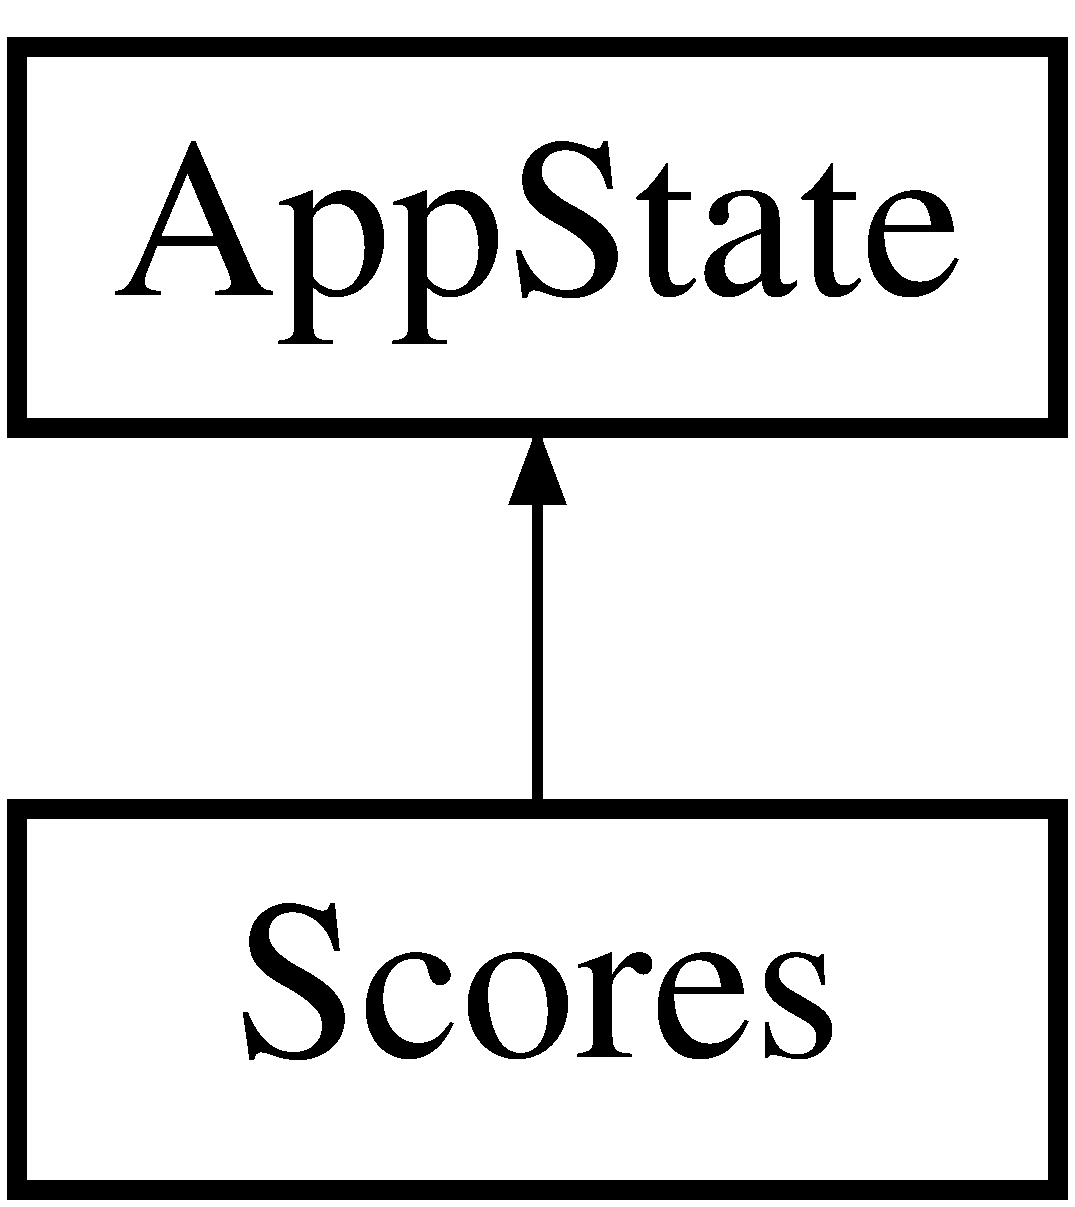
\includegraphics[height=2.000000cm]{class_scores}
\end{center}
\end{figure}
\subsection*{Metody publiczne}
\begin{DoxyCompactItemize}
\item 
\hyperlink{class_scores_a2fa6bcad8977919743d5af197f178c84}{Scores} ()
\item 
\hyperlink{class_scores_a911d7590e2708759f26c585ecdbf6a89}{Scores} (std\+::vector$<$ \hyperlink{class_player}{Player} $\ast$ $>$ players, int level, bool game\+\_\+over)
\item 
bool \hyperlink{class_scores_ace5dca138217e9bc5b18871b9ea9764b}{finished} () const 
\item 
void \hyperlink{class_scores_a9fb6838fe10b06aa9f439e3aae90a803}{draw} ()
\item 
void \hyperlink{class_scores_ae1eda4aec4cfc65c8bacb648ea28212e}{update} (Uint32 dt)
\item 
void \hyperlink{class_scores_ad6600e877a2b1c794cd1e849a7092d5e}{event\+Process} (S\+D\+L\+\_\+\+Event $\ast$ev)
\item 
\hyperlink{class_app_state}{App\+State} $\ast$ \hyperlink{class_scores_abd664c78d44381251db40ebba0e5b773}{next\+State} ()
\end{DoxyCompactItemize}


\subsection{Dokumentacja konstruktora i destruktora}
\hypertarget{class_scores_a2fa6bcad8977919743d5af197f178c84}{}\index{Scores@{Scores}!Scores@{Scores}}
\index{Scores@{Scores}!Scores@{Scores}}
\subsubsection[{Scores}]{\setlength{\rightskip}{0pt plus 5cm}Scores\+::\+Scores (
\begin{DoxyParamCaption}
{}
\end{DoxyParamCaption}
)}\label{class_scores_a2fa6bcad8977919743d5af197f178c84}
\hypertarget{class_scores_a911d7590e2708759f26c585ecdbf6a89}{}\index{Scores@{Scores}!Scores@{Scores}}
\index{Scores@{Scores}!Scores@{Scores}}
\subsubsection[{Scores}]{\setlength{\rightskip}{0pt plus 5cm}Scores\+::\+Scores (
\begin{DoxyParamCaption}
\item[{std\+::vector$<$ {\bf Player} $\ast$ $>$}]{players, }
\item[{int}]{level, }
\item[{bool}]{game\+\_\+over}
\end{DoxyParamCaption}
)}\label{class_scores_a911d7590e2708759f26c585ecdbf6a89}


\subsection{Dokumentacja funkcji składowych}
\hypertarget{class_scores_a9fb6838fe10b06aa9f439e3aae90a803}{}\index{Scores@{Scores}!draw@{draw}}
\index{draw@{draw}!Scores@{Scores}}
\subsubsection[{draw}]{\setlength{\rightskip}{0pt plus 5cm}void Scores\+::draw (
\begin{DoxyParamCaption}
{}
\end{DoxyParamCaption}
)\hspace{0.3cm}{\ttfamily [virtual]}}\label{class_scores_a9fb6838fe10b06aa9f439e3aae90a803}
Funkcja rysująca elementy gry należące do danego stanu 

Implementuje \hyperlink{class_app_state_ad2a668dc35b06c330a788e82d9eebee2}{App\+State}.

\hypertarget{class_scores_ad6600e877a2b1c794cd1e849a7092d5e}{}\index{Scores@{Scores}!event\+Process@{event\+Process}}
\index{event\+Process@{event\+Process}!Scores@{Scores}}
\subsubsection[{event\+Process}]{\setlength{\rightskip}{0pt plus 5cm}void Scores\+::event\+Process (
\begin{DoxyParamCaption}
\item[{S\+D\+L\+\_\+\+Event $\ast$}]{ev}
\end{DoxyParamCaption}
)\hspace{0.3cm}{\ttfamily [virtual]}}\label{class_scores_ad6600e877a2b1c794cd1e849a7092d5e}
Funkcja umożliwiająca obsługę zdarzeń wykrywanych przez bibliotekę S\+D\+L2. 
\begin{DoxyParams}{Parametry}
{\em ev} & -\/ wskaźnik na unię S\+D\+L\+\_\+\+Event przechowującą typ i parametry różnych zdarzeń \\
\hline
\end{DoxyParams}


Implementuje \hyperlink{class_app_state_a9cd9175e5cd251bea2e7eeb4ee9f6137}{App\+State}.

\hypertarget{class_scores_ace5dca138217e9bc5b18871b9ea9764b}{}\index{Scores@{Scores}!finished@{finished}}
\index{finished@{finished}!Scores@{Scores}}
\subsubsection[{finished}]{\setlength{\rightskip}{0pt plus 5cm}bool Scores\+::finished (
\begin{DoxyParamCaption}
{}
\end{DoxyParamCaption}
) const\hspace{0.3cm}{\ttfamily [virtual]}}\label{class_scores_ace5dca138217e9bc5b18871b9ea9764b}
Funkcja sprawdza czy aktualny stan gry się skończył. \begin{DoxyReturn}{Zwraca}
{\itshape true} jeżeli obecny stan gry się skończył, w przeciwnym wypadku {\itshape false}. 
\end{DoxyReturn}


Implementuje \hyperlink{class_app_state_ad377464581817ae4000b9cd6c47dc4e8}{App\+State}.

\hypertarget{class_scores_abd664c78d44381251db40ebba0e5b773}{}\index{Scores@{Scores}!next\+State@{next\+State}}
\index{next\+State@{next\+State}!Scores@{Scores}}
\subsubsection[{next\+State}]{\setlength{\rightskip}{0pt plus 5cm}{\bf App\+State} $\ast$ Scores\+::next\+State (
\begin{DoxyParamCaption}
{}
\end{DoxyParamCaption}
)\hspace{0.3cm}{\ttfamily [virtual]}}\label{class_scores_abd664c78d44381251db40ebba0e5b773}
Funkcja zwracającya następny stan po zakończeniu obecnego. Funkcję należy wywołać tylko wtedy, gdy funkcja {\itshape finished} zwróci wartość 1. \begin{DoxyReturn}{Zwraca}
następny stan gry 
\end{DoxyReturn}


Implementuje \hyperlink{class_app_state_afafba64bbaaf7552f6e0632821c2338f}{App\+State}.

\hypertarget{class_scores_ae1eda4aec4cfc65c8bacb648ea28212e}{}\index{Scores@{Scores}!update@{update}}
\index{update@{update}!Scores@{Scores}}
\subsubsection[{update}]{\setlength{\rightskip}{0pt plus 5cm}void Scores\+::update (
\begin{DoxyParamCaption}
\item[{Uint32}]{dt}
\end{DoxyParamCaption}
)\hspace{0.3cm}{\ttfamily [virtual]}}\label{class_scores_ae1eda4aec4cfc65c8bacb648ea28212e}
Funkcja aktualizująca stan obiektów i liczników w grze 
\begin{DoxyParams}{Parametry}
{\em dt} & -\/ czas od ostatniego wywołania funkcji w milisekundach \\
\hline
\end{DoxyParams}


Implementuje \hyperlink{class_app_state_a28660de31b5a7a36691b67866f82e5f2}{App\+State}.



Dokumentacja dla tej klasy została wygenerowana z plików\+:\begin{DoxyCompactItemize}
\item 
src/app\+\_\+state/\hyperlink{scores_8h}{scores.\+h}\item 
src/app\+\_\+state/\hyperlink{scores_8cpp}{scores.\+cpp}\end{DoxyCompactItemize}

\hypertarget{class_sprite_config}{}\section{Dokumentacja klasy Sprite\+Config}
\label{class_sprite_config}\index{Sprite\+Config@{Sprite\+Config}}


{\ttfamily \#include $<$spriteconfig.\+h$>$}

\subsection*{Metody publiczne}
\begin{DoxyCompactItemize}
\item 
\hyperlink{class_sprite_config_ae050a6bd2853271b140031e483f9a18d}{Sprite\+Config} ()
\item 
const \hyperlink{struct_sprite_data}{Sprite\+Data} $\ast$ \hyperlink{class_sprite_config_a347c7f41a0cba1a15f4c0e9c90f57499}{get\+Sprite\+Data} (\hyperlink{type_8h_ac6fa10729dffeb6a192492f13c25e31a}{Sprite\+Type} sp) const 
\end{DoxyCompactItemize}


\subsection{Dokumentacja konstruktora i destruktora}
\hypertarget{class_sprite_config_ae050a6bd2853271b140031e483f9a18d}{}\index{Sprite\+Config@{Sprite\+Config}!Sprite\+Config@{Sprite\+Config}}
\index{Sprite\+Config@{Sprite\+Config}!Sprite\+Config@{Sprite\+Config}}
\subsubsection[{Sprite\+Config}]{\setlength{\rightskip}{0pt plus 5cm}Sprite\+Config\+::\+Sprite\+Config (
\begin{DoxyParamCaption}
{}
\end{DoxyParamCaption}
)}\label{class_sprite_config_ae050a6bd2853271b140031e483f9a18d}


\subsection{Dokumentacja funkcji składowych}
\hypertarget{class_sprite_config_a347c7f41a0cba1a15f4c0e9c90f57499}{}\index{Sprite\+Config@{Sprite\+Config}!get\+Sprite\+Data@{get\+Sprite\+Data}}
\index{get\+Sprite\+Data@{get\+Sprite\+Data}!Sprite\+Config@{Sprite\+Config}}
\subsubsection[{get\+Sprite\+Data}]{\setlength{\rightskip}{0pt plus 5cm}const {\bf Sprite\+Data} $\ast$ Sprite\+Config\+::get\+Sprite\+Data (
\begin{DoxyParamCaption}
\item[{{\bf Sprite\+Type}}]{sp}
\end{DoxyParamCaption}
) const}\label{class_sprite_config_a347c7f41a0cba1a15f4c0e9c90f57499}


Dokumentacja dla tej klasy została wygenerowana z plików\+:\begin{DoxyCompactItemize}
\item 
src/engine/\hyperlink{spriteconfig_8h}{spriteconfig.\+h}\item 
src/engine/\hyperlink{spriteconfig_8cpp}{spriteconfig.\+cpp}\end{DoxyCompactItemize}

\hypertarget{struct_sprite_data}{}\section{Dokumentacja struktury Sprite\+Data}
\label{struct_sprite_data}\index{Sprite\+Data@{Sprite\+Data}}


{\ttfamily \#include $<$spriteconfig.\+h$>$}

\subsection*{Metody publiczne}
\begin{DoxyCompactItemize}
\item 
\hyperlink{struct_sprite_data_a180d297cf3681064f9fbc5e63418c981}{Sprite\+Data} ()
\item 
\hyperlink{struct_sprite_data_a9c196ade0d0e8b8456216e53100b459d}{Sprite\+Data} (int x, int y, int w, int h, int fc, int fd, bool l)
\end{DoxyCompactItemize}
\subsection*{Atrybuty publiczne}
\begin{DoxyCompactItemize}
\item 
S\+D\+L\+\_\+\+Rect \hyperlink{struct_sprite_data_ad4482d398fce500b0e4a0f408a2ddd49}{rect}
\item 
int \hyperlink{struct_sprite_data_aafe351d09e5676b4960124f80be55d8c}{frames\+\_\+count}
\item 
unsigned \hyperlink{struct_sprite_data_ad0223b5392f02bf68ec30169fbdafd52}{frame\+\_\+duration}
\item 
bool \hyperlink{struct_sprite_data_a0833cf779f1fb40ae68048e2dc1ebb43}{loop}
\end{DoxyCompactItemize}


\subsection{Dokumentacja konstruktora i destruktora}
\hypertarget{struct_sprite_data_a180d297cf3681064f9fbc5e63418c981}{}\index{Sprite\+Data@{Sprite\+Data}!Sprite\+Data@{Sprite\+Data}}
\index{Sprite\+Data@{Sprite\+Data}!Sprite\+Data@{Sprite\+Data}}
\subsubsection[{Sprite\+Data}]{\setlength{\rightskip}{0pt plus 5cm}Sprite\+Data\+::\+Sprite\+Data (
\begin{DoxyParamCaption}
{}
\end{DoxyParamCaption}
)\hspace{0.3cm}{\ttfamily [inline]}}\label{struct_sprite_data_a180d297cf3681064f9fbc5e63418c981}
\hypertarget{struct_sprite_data_a9c196ade0d0e8b8456216e53100b459d}{}\index{Sprite\+Data@{Sprite\+Data}!Sprite\+Data@{Sprite\+Data}}
\index{Sprite\+Data@{Sprite\+Data}!Sprite\+Data@{Sprite\+Data}}
\subsubsection[{Sprite\+Data}]{\setlength{\rightskip}{0pt plus 5cm}Sprite\+Data\+::\+Sprite\+Data (
\begin{DoxyParamCaption}
\item[{int}]{x, }
\item[{int}]{y, }
\item[{int}]{w, }
\item[{int}]{h, }
\item[{int}]{fc, }
\item[{int}]{fd, }
\item[{bool}]{l}
\end{DoxyParamCaption}
)\hspace{0.3cm}{\ttfamily [inline]}}\label{struct_sprite_data_a9c196ade0d0e8b8456216e53100b459d}


\subsection{Dokumentacja atrybutów składowych}
\hypertarget{struct_sprite_data_ad0223b5392f02bf68ec30169fbdafd52}{}\index{Sprite\+Data@{Sprite\+Data}!frame\+\_\+duration@{frame\+\_\+duration}}
\index{frame\+\_\+duration@{frame\+\_\+duration}!Sprite\+Data@{Sprite\+Data}}
\subsubsection[{frame\+\_\+duration}]{\setlength{\rightskip}{0pt plus 5cm}unsigned Sprite\+Data\+::frame\+\_\+duration}\label{struct_sprite_data_ad0223b5392f02bf68ec30169fbdafd52}
\hypertarget{struct_sprite_data_aafe351d09e5676b4960124f80be55d8c}{}\index{Sprite\+Data@{Sprite\+Data}!frames\+\_\+count@{frames\+\_\+count}}
\index{frames\+\_\+count@{frames\+\_\+count}!Sprite\+Data@{Sprite\+Data}}
\subsubsection[{frames\+\_\+count}]{\setlength{\rightskip}{0pt plus 5cm}int Sprite\+Data\+::frames\+\_\+count}\label{struct_sprite_data_aafe351d09e5676b4960124f80be55d8c}
\hypertarget{struct_sprite_data_a0833cf779f1fb40ae68048e2dc1ebb43}{}\index{Sprite\+Data@{Sprite\+Data}!loop@{loop}}
\index{loop@{loop}!Sprite\+Data@{Sprite\+Data}}
\subsubsection[{loop}]{\setlength{\rightskip}{0pt plus 5cm}bool Sprite\+Data\+::loop}\label{struct_sprite_data_a0833cf779f1fb40ae68048e2dc1ebb43}
\hypertarget{struct_sprite_data_ad4482d398fce500b0e4a0f408a2ddd49}{}\index{Sprite\+Data@{Sprite\+Data}!rect@{rect}}
\index{rect@{rect}!Sprite\+Data@{Sprite\+Data}}
\subsubsection[{rect}]{\setlength{\rightskip}{0pt plus 5cm}S\+D\+L\+\_\+\+Rect Sprite\+Data\+::rect}\label{struct_sprite_data_ad4482d398fce500b0e4a0f408a2ddd49}


Dokumentacja dla tej struktury została wygenerowana z pliku\+:\begin{DoxyCompactItemize}
\item 
src/engine/\hyperlink{spriteconfig_8h}{spriteconfig.\+h}\end{DoxyCompactItemize}

\hypertarget{class_tank}{}\section{Dokumentacja klasy Tank}
\label{class_tank}\index{Tank@{Tank}}


{\ttfamily \#include $<$tank.\+h$>$}

Diagram dziedziczenia dla Tank\begin{figure}[H]
\begin{center}
\leavevmode
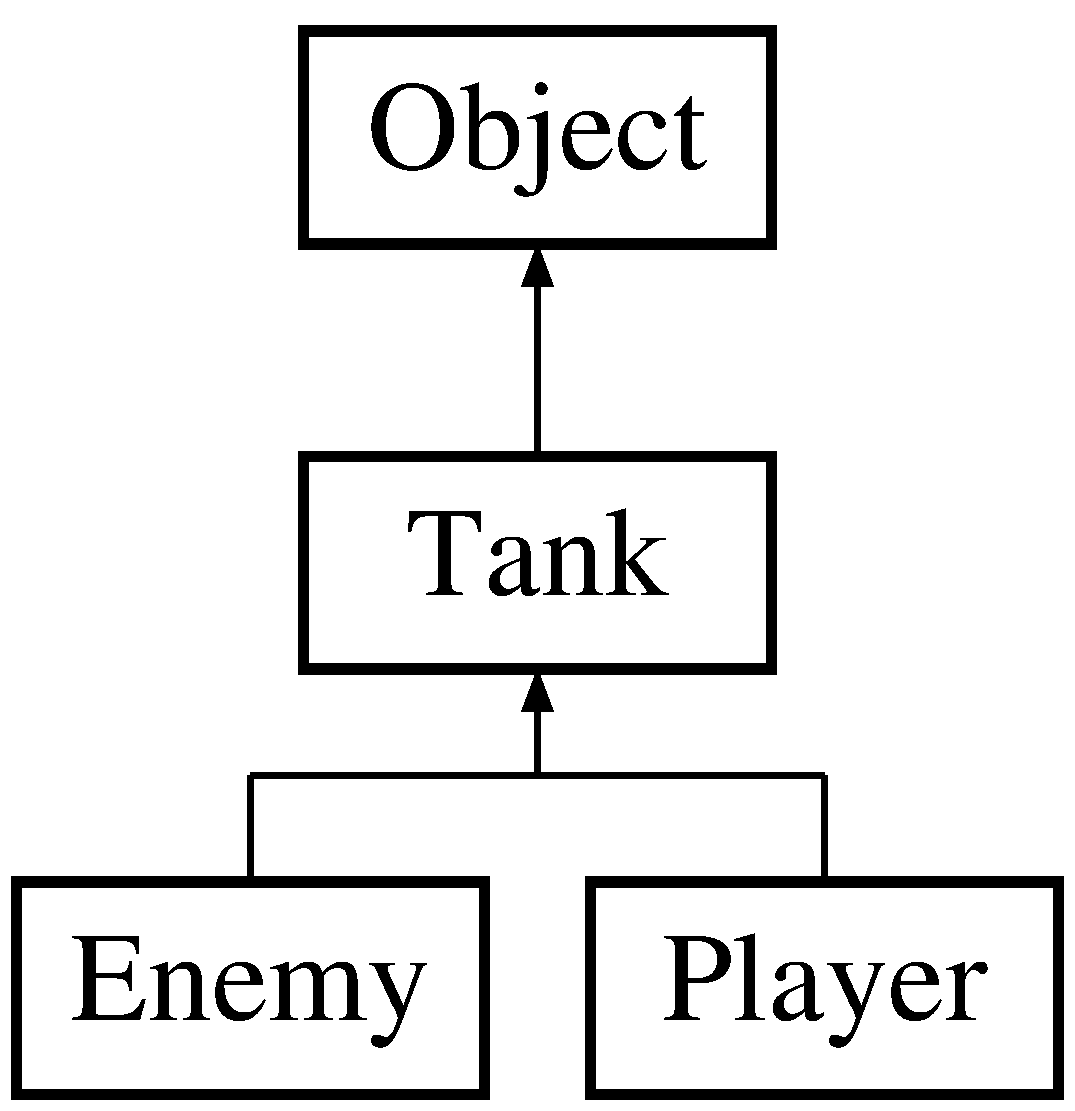
\includegraphics[height=3.000000cm]{class_tank}
\end{center}
\end{figure}
\subsection*{Metody publiczne}
\begin{DoxyCompactItemize}
\item 
\hyperlink{class_tank_ae8be1e2c9376c3a4590b4bf689eaed76}{Tank} ()
\item 
\hyperlink{class_tank_ab6b6a6d0ec3994fa12f4933602dd4325}{Tank} (double x, double y, \hyperlink{type_8h_ac6fa10729dffeb6a192492f13c25e31a}{Sprite\+Type} \hyperlink{class_object_a1b89f32cd9e0040f8a2455f3cef7d0d2}{type})
\item 
virtual \hyperlink{class_tank_a9e4fce49ae7fe871894c1a3122c10269}{$\sim$\+Tank} ()
\item 
void \hyperlink{class_tank_ab30c54bb7378b522fa965d4e8ab7ed4f}{draw} ()
\item 
void \hyperlink{class_tank_a1278dfec0f2d1d3bb1f4ce0a19957c0f}{update} (Uint32 dt)
\item 
virtual \hyperlink{class_bullet}{Bullet} $\ast$ \hyperlink{class_tank_ae5c683a77507d638b2e2d7526e5205de}{fire} ()
\item 
S\+D\+L\+\_\+\+Rect \hyperlink{class_tank_a2373592e898ce038e22ed59f4486ba6d}{next\+Collision\+Rect} (Uint32 dt)
\item 
void \hyperlink{class_tank_a649b24d19a48a3e93f4ba14821338f46}{set\+Direction} (\hyperlink{type_8h_a224b9163917ac32fc95a60d8c1eec3aa}{Direction} d)
\item 
void \hyperlink{class_tank_a4d254f913ab43a6bc62494a8ab1444cd}{collide} ()
\item 
virtual void \hyperlink{class_tank_a61501e1b99fd235500b79f39c6b2fc8f}{respawn} ()
\item 
virtual void \hyperlink{class_tank_a5d2e3302417166ccdc42b8bc2e5d5dc4}{destroy} ()
\item 
void \hyperlink{class_tank_a4c624b0a64ca72567a758d17b3350873}{set\+Flag} (\hyperlink{type_8h_a4cfefb8efe4714111e829031e2df4faf}{Tank\+State\+Flag} flag)
\item 
void \hyperlink{class_tank_ac8525d73bc6bd199ca51bb447f342925}{clear\+Flag} (\hyperlink{type_8h_a4cfefb8efe4714111e829031e2df4faf}{Tank\+State\+Flag} flag)
\item 
bool \hyperlink{class_tank_ab9d5c0e134f6be71b7bc245268e90a01}{test\+Flag} (\hyperlink{type_8h_a4cfefb8efe4714111e829031e2df4faf}{Tank\+State\+Flag} flag)
\end{DoxyCompactItemize}
\subsection*{Atrybuty publiczne}
\begin{DoxyCompactItemize}
\item 
double \hyperlink{class_tank_acd370abc3ccd4c67c8285e42884c7b1c}{default\+\_\+speed}
\item 
double \hyperlink{class_tank_a4c19847eec64e4d3793885150145aa93}{speed}
\item 
bool \hyperlink{class_tank_a4134e3bc03ed6453f1e76f161f29a657}{stop}
\item 
\hyperlink{type_8h_a224b9163917ac32fc95a60d8c1eec3aa}{Direction} \hyperlink{class_tank_a316c67f799b64265a676038da73b0676}{direction}
\item 
std\+::vector$<$ \hyperlink{class_bullet}{Bullet} $\ast$ $>$ \hyperlink{class_tank_a85d5a28cc0e589748644bdf2879745cb}{bullets}
\item 
int \hyperlink{class_tank_abb0e870d0f5ecdb44adf6c1136536822}{lives\+\_\+count}
\end{DoxyCompactItemize}
\subsection*{Atrybuty chronione}
\begin{DoxyCompactItemize}
\item 
\hyperlink{tank_8h_a7109342eb8cc7d8bbf8b6309ebcb4669}{Tank\+State\+Flags} \hyperlink{class_tank_a20c5abbc8ee4901444f0fc1c9fd46eb1}{m\+\_\+flags}
\item 
Sint32 \hyperlink{class_tank_aee43131c389c141d21ac58f3a6dbb025}{m\+\_\+slip\+\_\+time}
\item 
\hyperlink{type_8h_a224b9163917ac32fc95a60d8c1eec3aa}{Direction} \hyperlink{class_tank_a4411d9cf4dd459296b320e36d08e7f12}{new\+\_\+direction}
\item 
unsigned \hyperlink{class_tank_a2a6fb83df6ad84e8b3145f36d25b0ced}{m\+\_\+bullet\+\_\+max\+\_\+size}
\item 
\hyperlink{class_object}{Object} $\ast$ \hyperlink{class_tank_a19dc0d8574c701ea45c3ba7c610c5aa4}{m\+\_\+shield}
\item 
\hyperlink{class_object}{Object} $\ast$ \hyperlink{class_tank_afc71fe83709cbe9df5413f04213a5a3b}{m\+\_\+boat}
\item 
Uint32 \hyperlink{class_tank_ad6f78705b79f5570f403dea866c970f8}{m\+\_\+shield\+\_\+time}
\item 
Uint32 \hyperlink{class_tank_a98f872a3bd144261ca25569091be8ab6}{m\+\_\+frozen\+\_\+time}
\end{DoxyCompactItemize}
\subsection*{Dodatkowe Dziedziczone Składowe}


\subsection{Dokumentacja konstruktora i destruktora}
\hypertarget{class_tank_ae8be1e2c9376c3a4590b4bf689eaed76}{}\index{Tank@{Tank}!Tank@{Tank}}
\index{Tank@{Tank}!Tank@{Tank}}
\subsubsection[{Tank}]{\setlength{\rightskip}{0pt plus 5cm}Tank\+::\+Tank (
\begin{DoxyParamCaption}
{}
\end{DoxyParamCaption}
)}\label{class_tank_ae8be1e2c9376c3a4590b4bf689eaed76}
\hypertarget{class_tank_ab6b6a6d0ec3994fa12f4933602dd4325}{}\index{Tank@{Tank}!Tank@{Tank}}
\index{Tank@{Tank}!Tank@{Tank}}
\subsubsection[{Tank}]{\setlength{\rightskip}{0pt plus 5cm}Tank\+::\+Tank (
\begin{DoxyParamCaption}
\item[{double}]{x, }
\item[{double}]{y, }
\item[{{\bf Sprite\+Type}}]{type}
\end{DoxyParamCaption}
)}\label{class_tank_ab6b6a6d0ec3994fa12f4933602dd4325}
\hypertarget{class_tank_a9e4fce49ae7fe871894c1a3122c10269}{}\index{Tank@{Tank}!````~Tank@{$\sim$\+Tank}}
\index{````~Tank@{$\sim$\+Tank}!Tank@{Tank}}
\subsubsection[{$\sim$\+Tank}]{\setlength{\rightskip}{0pt plus 5cm}Tank\+::$\sim$\+Tank (
\begin{DoxyParamCaption}
{}
\end{DoxyParamCaption}
)\hspace{0.3cm}{\ttfamily [virtual]}}\label{class_tank_a9e4fce49ae7fe871894c1a3122c10269}


\subsection{Dokumentacja funkcji składowych}
\hypertarget{class_tank_ac8525d73bc6bd199ca51bb447f342925}{}\index{Tank@{Tank}!clear\+Flag@{clear\+Flag}}
\index{clear\+Flag@{clear\+Flag}!Tank@{Tank}}
\subsubsection[{clear\+Flag}]{\setlength{\rightskip}{0pt plus 5cm}void Tank\+::clear\+Flag (
\begin{DoxyParamCaption}
\item[{{\bf Tank\+State\+Flag}}]{flag}
\end{DoxyParamCaption}
)}\label{class_tank_ac8525d73bc6bd199ca51bb447f342925}
\hypertarget{class_tank_a4d254f913ab43a6bc62494a8ab1444cd}{}\index{Tank@{Tank}!collide@{collide}}
\index{collide@{collide}!Tank@{Tank}}
\subsubsection[{collide}]{\setlength{\rightskip}{0pt plus 5cm}void Tank\+::collide (
\begin{DoxyParamCaption}
{}
\end{DoxyParamCaption}
)}\label{class_tank_a4d254f913ab43a6bc62494a8ab1444cd}
\hypertarget{class_tank_a5d2e3302417166ccdc42b8bc2e5d5dc4}{}\index{Tank@{Tank}!destroy@{destroy}}
\index{destroy@{destroy}!Tank@{Tank}}
\subsubsection[{destroy}]{\setlength{\rightskip}{0pt plus 5cm}void Tank\+::destroy (
\begin{DoxyParamCaption}
{}
\end{DoxyParamCaption}
)\hspace{0.3cm}{\ttfamily [virtual]}}\label{class_tank_a5d2e3302417166ccdc42b8bc2e5d5dc4}


Reimplementowana w \hyperlink{class_player_acb40d0a5d388029d48156fb06fdd288c}{Player} i \hyperlink{class_enemy_a296a5757097f271eb01284eabb064715}{Enemy}.

\hypertarget{class_tank_ab30c54bb7378b522fa965d4e8ab7ed4f}{}\index{Tank@{Tank}!draw@{draw}}
\index{draw@{draw}!Tank@{Tank}}
\subsubsection[{draw}]{\setlength{\rightskip}{0pt plus 5cm}void Tank\+::draw (
\begin{DoxyParamCaption}
{}
\end{DoxyParamCaption}
)\hspace{0.3cm}{\ttfamily [virtual]}}\label{class_tank_ab30c54bb7378b522fa965d4e8ab7ed4f}


Reimplementowana z \hyperlink{class_object_a821f5b25b450fa1acdb3f9c0b5962592}{Object}.

\hypertarget{class_tank_ae5c683a77507d638b2e2d7526e5205de}{}\index{Tank@{Tank}!fire@{fire}}
\index{fire@{fire}!Tank@{Tank}}
\subsubsection[{fire}]{\setlength{\rightskip}{0pt plus 5cm}{\bf Bullet} $\ast$ Tank\+::fire (
\begin{DoxyParamCaption}
{}
\end{DoxyParamCaption}
)\hspace{0.3cm}{\ttfamily [virtual]}}\label{class_tank_ae5c683a77507d638b2e2d7526e5205de}


Reimplementowana w \hyperlink{class_player_a5f0f389fdf5d685f088a997ed5af925d}{Player}.

\hypertarget{class_tank_a2373592e898ce038e22ed59f4486ba6d}{}\index{Tank@{Tank}!next\+Collision\+Rect@{next\+Collision\+Rect}}
\index{next\+Collision\+Rect@{next\+Collision\+Rect}!Tank@{Tank}}
\subsubsection[{next\+Collision\+Rect}]{\setlength{\rightskip}{0pt plus 5cm}S\+D\+L\+\_\+\+Rect Tank\+::next\+Collision\+Rect (
\begin{DoxyParamCaption}
\item[{Uint32}]{dt}
\end{DoxyParamCaption}
)}\label{class_tank_a2373592e898ce038e22ed59f4486ba6d}
\hypertarget{class_tank_a61501e1b99fd235500b79f39c6b2fc8f}{}\index{Tank@{Tank}!respawn@{respawn}}
\index{respawn@{respawn}!Tank@{Tank}}
\subsubsection[{respawn}]{\setlength{\rightskip}{0pt plus 5cm}void Tank\+::respawn (
\begin{DoxyParamCaption}
{}
\end{DoxyParamCaption}
)\hspace{0.3cm}{\ttfamily [virtual]}}\label{class_tank_a61501e1b99fd235500b79f39c6b2fc8f}


Reimplementowana w \hyperlink{class_player_a038a74bd768b6eec8fbe57cb2bacf811}{Player}.

\hypertarget{class_tank_a649b24d19a48a3e93f4ba14821338f46}{}\index{Tank@{Tank}!set\+Direction@{set\+Direction}}
\index{set\+Direction@{set\+Direction}!Tank@{Tank}}
\subsubsection[{set\+Direction}]{\setlength{\rightskip}{0pt plus 5cm}void Tank\+::set\+Direction (
\begin{DoxyParamCaption}
\item[{{\bf Direction}}]{d}
\end{DoxyParamCaption}
)}\label{class_tank_a649b24d19a48a3e93f4ba14821338f46}
\hypertarget{class_tank_a4c624b0a64ca72567a758d17b3350873}{}\index{Tank@{Tank}!set\+Flag@{set\+Flag}}
\index{set\+Flag@{set\+Flag}!Tank@{Tank}}
\subsubsection[{set\+Flag}]{\setlength{\rightskip}{0pt plus 5cm}void Tank\+::set\+Flag (
\begin{DoxyParamCaption}
\item[{{\bf Tank\+State\+Flag}}]{flag}
\end{DoxyParamCaption}
)}\label{class_tank_a4c624b0a64ca72567a758d17b3350873}
\hypertarget{class_tank_ab9d5c0e134f6be71b7bc245268e90a01}{}\index{Tank@{Tank}!test\+Flag@{test\+Flag}}
\index{test\+Flag@{test\+Flag}!Tank@{Tank}}
\subsubsection[{test\+Flag}]{\setlength{\rightskip}{0pt plus 5cm}bool Tank\+::test\+Flag (
\begin{DoxyParamCaption}
\item[{{\bf Tank\+State\+Flag}}]{flag}
\end{DoxyParamCaption}
)}\label{class_tank_ab9d5c0e134f6be71b7bc245268e90a01}
\hypertarget{class_tank_a1278dfec0f2d1d3bb1f4ce0a19957c0f}{}\index{Tank@{Tank}!update@{update}}
\index{update@{update}!Tank@{Tank}}
\subsubsection[{update}]{\setlength{\rightskip}{0pt plus 5cm}void Tank\+::update (
\begin{DoxyParamCaption}
\item[{Uint32}]{dt}
\end{DoxyParamCaption}
)\hspace{0.3cm}{\ttfamily [virtual]}}\label{class_tank_a1278dfec0f2d1d3bb1f4ce0a19957c0f}


Reimplementowana z \hyperlink{class_object_a02c1621329cb9ec5268072a2402d2ac5}{Object}.



\subsection{Dokumentacja atrybutów składowych}
\hypertarget{class_tank_a85d5a28cc0e589748644bdf2879745cb}{}\index{Tank@{Tank}!bullets@{bullets}}
\index{bullets@{bullets}!Tank@{Tank}}
\subsubsection[{bullets}]{\setlength{\rightskip}{0pt plus 5cm}std\+::vector$<${\bf Bullet}$\ast$$>$ Tank\+::bullets}\label{class_tank_a85d5a28cc0e589748644bdf2879745cb}
\hypertarget{class_tank_acd370abc3ccd4c67c8285e42884c7b1c}{}\index{Tank@{Tank}!default\+\_\+speed@{default\+\_\+speed}}
\index{default\+\_\+speed@{default\+\_\+speed}!Tank@{Tank}}
\subsubsection[{default\+\_\+speed}]{\setlength{\rightskip}{0pt plus 5cm}double Tank\+::default\+\_\+speed}\label{class_tank_acd370abc3ccd4c67c8285e42884c7b1c}
\hypertarget{class_tank_a316c67f799b64265a676038da73b0676}{}\index{Tank@{Tank}!direction@{direction}}
\index{direction@{direction}!Tank@{Tank}}
\subsubsection[{direction}]{\setlength{\rightskip}{0pt plus 5cm}{\bf Direction} Tank\+::direction}\label{class_tank_a316c67f799b64265a676038da73b0676}
\hypertarget{class_tank_abb0e870d0f5ecdb44adf6c1136536822}{}\index{Tank@{Tank}!lives\+\_\+count@{lives\+\_\+count}}
\index{lives\+\_\+count@{lives\+\_\+count}!Tank@{Tank}}
\subsubsection[{lives\+\_\+count}]{\setlength{\rightskip}{0pt plus 5cm}int Tank\+::lives\+\_\+count}\label{class_tank_abb0e870d0f5ecdb44adf6c1136536822}
\hypertarget{class_tank_afc71fe83709cbe9df5413f04213a5a3b}{}\index{Tank@{Tank}!m\+\_\+boat@{m\+\_\+boat}}
\index{m\+\_\+boat@{m\+\_\+boat}!Tank@{Tank}}
\subsubsection[{m\+\_\+boat}]{\setlength{\rightskip}{0pt plus 5cm}{\bf Object}$\ast$ Tank\+::m\+\_\+boat\hspace{0.3cm}{\ttfamily [protected]}}\label{class_tank_afc71fe83709cbe9df5413f04213a5a3b}
\hypertarget{class_tank_a2a6fb83df6ad84e8b3145f36d25b0ced}{}\index{Tank@{Tank}!m\+\_\+bullet\+\_\+max\+\_\+size@{m\+\_\+bullet\+\_\+max\+\_\+size}}
\index{m\+\_\+bullet\+\_\+max\+\_\+size@{m\+\_\+bullet\+\_\+max\+\_\+size}!Tank@{Tank}}
\subsubsection[{m\+\_\+bullet\+\_\+max\+\_\+size}]{\setlength{\rightskip}{0pt plus 5cm}unsigned Tank\+::m\+\_\+bullet\+\_\+max\+\_\+size\hspace{0.3cm}{\ttfamily [protected]}}\label{class_tank_a2a6fb83df6ad84e8b3145f36d25b0ced}
\hypertarget{class_tank_a20c5abbc8ee4901444f0fc1c9fd46eb1}{}\index{Tank@{Tank}!m\+\_\+flags@{m\+\_\+flags}}
\index{m\+\_\+flags@{m\+\_\+flags}!Tank@{Tank}}
\subsubsection[{m\+\_\+flags}]{\setlength{\rightskip}{0pt plus 5cm}{\bf Tank\+State\+Flags} Tank\+::m\+\_\+flags\hspace{0.3cm}{\ttfamily [protected]}}\label{class_tank_a20c5abbc8ee4901444f0fc1c9fd46eb1}
\hypertarget{class_tank_a98f872a3bd144261ca25569091be8ab6}{}\index{Tank@{Tank}!m\+\_\+frozen\+\_\+time@{m\+\_\+frozen\+\_\+time}}
\index{m\+\_\+frozen\+\_\+time@{m\+\_\+frozen\+\_\+time}!Tank@{Tank}}
\subsubsection[{m\+\_\+frozen\+\_\+time}]{\setlength{\rightskip}{0pt plus 5cm}Uint32 Tank\+::m\+\_\+frozen\+\_\+time\hspace{0.3cm}{\ttfamily [protected]}}\label{class_tank_a98f872a3bd144261ca25569091be8ab6}
\hypertarget{class_tank_a19dc0d8574c701ea45c3ba7c610c5aa4}{}\index{Tank@{Tank}!m\+\_\+shield@{m\+\_\+shield}}
\index{m\+\_\+shield@{m\+\_\+shield}!Tank@{Tank}}
\subsubsection[{m\+\_\+shield}]{\setlength{\rightskip}{0pt plus 5cm}{\bf Object}$\ast$ Tank\+::m\+\_\+shield\hspace{0.3cm}{\ttfamily [protected]}}\label{class_tank_a19dc0d8574c701ea45c3ba7c610c5aa4}
\hypertarget{class_tank_ad6f78705b79f5570f403dea866c970f8}{}\index{Tank@{Tank}!m\+\_\+shield\+\_\+time@{m\+\_\+shield\+\_\+time}}
\index{m\+\_\+shield\+\_\+time@{m\+\_\+shield\+\_\+time}!Tank@{Tank}}
\subsubsection[{m\+\_\+shield\+\_\+time}]{\setlength{\rightskip}{0pt plus 5cm}Uint32 Tank\+::m\+\_\+shield\+\_\+time\hspace{0.3cm}{\ttfamily [protected]}}\label{class_tank_ad6f78705b79f5570f403dea866c970f8}
\hypertarget{class_tank_aee43131c389c141d21ac58f3a6dbb025}{}\index{Tank@{Tank}!m\+\_\+slip\+\_\+time@{m\+\_\+slip\+\_\+time}}
\index{m\+\_\+slip\+\_\+time@{m\+\_\+slip\+\_\+time}!Tank@{Tank}}
\subsubsection[{m\+\_\+slip\+\_\+time}]{\setlength{\rightskip}{0pt plus 5cm}Sint32 Tank\+::m\+\_\+slip\+\_\+time\hspace{0.3cm}{\ttfamily [protected]}}\label{class_tank_aee43131c389c141d21ac58f3a6dbb025}
\hypertarget{class_tank_a4411d9cf4dd459296b320e36d08e7f12}{}\index{Tank@{Tank}!new\+\_\+direction@{new\+\_\+direction}}
\index{new\+\_\+direction@{new\+\_\+direction}!Tank@{Tank}}
\subsubsection[{new\+\_\+direction}]{\setlength{\rightskip}{0pt plus 5cm}{\bf Direction} Tank\+::new\+\_\+direction\hspace{0.3cm}{\ttfamily [protected]}}\label{class_tank_a4411d9cf4dd459296b320e36d08e7f12}
\hypertarget{class_tank_a4c19847eec64e4d3793885150145aa93}{}\index{Tank@{Tank}!speed@{speed}}
\index{speed@{speed}!Tank@{Tank}}
\subsubsection[{speed}]{\setlength{\rightskip}{0pt plus 5cm}double Tank\+::speed}\label{class_tank_a4c19847eec64e4d3793885150145aa93}
\hypertarget{class_tank_a4134e3bc03ed6453f1e76f161f29a657}{}\index{Tank@{Tank}!stop@{stop}}
\index{stop@{stop}!Tank@{Tank}}
\subsubsection[{stop}]{\setlength{\rightskip}{0pt plus 5cm}bool Tank\+::stop}\label{class_tank_a4134e3bc03ed6453f1e76f161f29a657}


Dokumentacja dla tej klasy została wygenerowana z plików\+:\begin{DoxyCompactItemize}
\item 
src/objects/\hyperlink{tank_8h}{tank.\+h}\item 
src/objects/\hyperlink{tank_8cpp}{tank.\+cpp}\end{DoxyCompactItemize}

\chapter{Dokumentacja plików}
\hypertarget{app_8cpp}{}\section{Dokumentacja pliku src/app.cpp}
\label{app_8cpp}\index{src/app.\+cpp@{src/app.\+cpp}}
{\ttfamily \#include \char`\"{}app.\+h\char`\"{}}\\*
{\ttfamily \#include \char`\"{}appconfig.\+h\char`\"{}}\\*
{\ttfamily \#include \char`\"{}engine/engine.\+h\char`\"{}}\\*
{\ttfamily \#include \char`\"{}app\+\_\+state/game.\+h\char`\"{}}\\*
{\ttfamily \#include \char`\"{}app\+\_\+state/menu.\+h\char`\"{}}\\*
{\ttfamily \#include $<$ctime$>$}\\*
{\ttfamily \#include $<$iostream$>$}\\*
{\ttfamily \#include $<$stdlib.\+h$>$}\\*
{\ttfamily \#include $<$S\+D\+L2/\+S\+D\+L.\+h$>$}\\*
{\ttfamily \#include $<$S\+D\+L2/\+S\+D\+L\+\_\+image.\+h$>$}\\*
{\ttfamily \#include $<$S\+D\+L2/\+S\+D\+L\+\_\+ttf.\+h$>$}\\*
\subsection*{Definicje}
\begin{DoxyCompactItemize}
\item 
\#define \hyperlink{app_8cpp_a1c6d5de492ac61ad29aec7aa9a436bbf}{V\+E\+R\+S\+I\+O\+N}~\char`\"{}1.\+0.\+0\char`\"{}
\end{DoxyCompactItemize}


\subsection{Dokumentacja definicji}
\hypertarget{app_8cpp_a1c6d5de492ac61ad29aec7aa9a436bbf}{}\index{app.\+cpp@{app.\+cpp}!V\+E\+R\+S\+I\+O\+N@{V\+E\+R\+S\+I\+O\+N}}
\index{V\+E\+R\+S\+I\+O\+N@{V\+E\+R\+S\+I\+O\+N}!app.\+cpp@{app.\+cpp}}
\subsubsection[{V\+E\+R\+S\+I\+O\+N}]{\setlength{\rightskip}{0pt plus 5cm}\#define V\+E\+R\+S\+I\+O\+N~\char`\"{}1.\+0.\+0\char`\"{}}\label{app_8cpp_a1c6d5de492ac61ad29aec7aa9a436bbf}

\hypertarget{app_8h}{}\section{Dokumentacja pliku src/app.h}
\label{app_8h}\index{src/app.\+h@{src/app.\+h}}
{\ttfamily \#include \char`\"{}app\+\_\+state/appstate.\+h\char`\"{}}\\*
\subsection*{Komponenty}
\begin{DoxyCompactItemize}
\item 
class \hyperlink{class_app}{App}
\end{DoxyCompactItemize}

\hypertarget{appstate_8h}{}\section{Dokumentacja pliku src/app\+\_\+state/appstate.h}
\label{appstate_8h}\index{src/app\+\_\+state/appstate.\+h@{src/app\+\_\+state/appstate.\+h}}
{\ttfamily \#include $<$S\+D\+L2/\+S\+D\+L\+\_\+events.\+h$>$}\\*
{\ttfamily \#include $<$string$>$}\\*
\subsection*{Komponenty}
\begin{DoxyCompactItemize}
\item 
class \hyperlink{class_app_state}{App\+State}
\begin{DoxyCompactList}\small\item\em Klasa jest interfejsem, po którym dziedziczą klasy {\itshape \hyperlink{class_game}{Game}}, {\itshape \hyperlink{class_menu}{Menu}}, {\itshape \hyperlink{class_scores}{Scores}}. \end{DoxyCompactList}\end{DoxyCompactItemize}

\hypertarget{game_8cpp}{}\section{Dokumentacja pliku src/app\+\_\+state/game.cpp}
\label{game_8cpp}\index{src/app\+\_\+state/game.\+cpp@{src/app\+\_\+state/game.\+cpp}}
{\ttfamily \#include \char`\"{}game.\+h\char`\"{}}\\*
{\ttfamily \#include \char`\"{}../engine/engine.\+h\char`\"{}}\\*
{\ttfamily \#include \char`\"{}../appconfig.\+h\char`\"{}}\\*
{\ttfamily \#include \char`\"{}menu.\+h\char`\"{}}\\*
{\ttfamily \#include \char`\"{}scores.\+h\char`\"{}}\\*
{\ttfamily \#include $<$S\+D\+L2/\+S\+D\+L.\+h$>$}\\*
{\ttfamily \#include $<$stdlib.\+h$>$}\\*
{\ttfamily \#include $<$ctime$>$}\\*
{\ttfamily \#include $<$fstream$>$}\\*
{\ttfamily \#include $<$algorithm$>$}\\*
{\ttfamily \#include $<$iostream$>$}\\*

\hypertarget{game_8h}{}\section{Dokumentacja pliku src/app\+\_\+state/game.h}
\label{game_8h}\index{src/app\+\_\+state/game.\+h@{src/app\+\_\+state/game.\+h}}
{\ttfamily \#include \char`\"{}appstate.\+h\char`\"{}}\\*
{\ttfamily \#include \char`\"{}../objects/object.\+h\char`\"{}}\\*
{\ttfamily \#include \char`\"{}../objects/player.\+h\char`\"{}}\\*
{\ttfamily \#include \char`\"{}../objects/enemy.\+h\char`\"{}}\\*
{\ttfamily \#include \char`\"{}../objects/bullet.\+h\char`\"{}}\\*
{\ttfamily \#include \char`\"{}../objects/brick.\+h\char`\"{}}\\*
{\ttfamily \#include \char`\"{}../objects/eagle.\+h\char`\"{}}\\*
{\ttfamily \#include \char`\"{}../objects/bonus.\+h\char`\"{}}\\*
{\ttfamily \#include $<$vector$>$}\\*
{\ttfamily \#include $<$string$>$}\\*
\subsection*{Komponenty}
\begin{DoxyCompactItemize}
\item 
class \hyperlink{class_game}{Game}
\begin{DoxyCompactList}\small\item\em Klasa odpowiada za ruch wszytkich czołgów oraz interaakcje między czołgami oraz między czołgami a innymi obiektami na mapie. \end{DoxyCompactList}\end{DoxyCompactItemize}

\hypertarget{menu_8cpp}{}\section{Dokumentacja pliku src/app\+\_\+state/menu.cpp}
\label{menu_8cpp}\index{src/app\+\_\+state/menu.\+cpp@{src/app\+\_\+state/menu.\+cpp}}
{\ttfamily \#include \char`\"{}menu.\+h\char`\"{}}\\*
{\ttfamily \#include \char`\"{}../engine/engine.\+h\char`\"{}}\\*
{\ttfamily \#include \char`\"{}../engine/renderer.\+h\char`\"{}}\\*
{\ttfamily \#include \char`\"{}../appconfig.\+h\char`\"{}}\\*
{\ttfamily \#include \char`\"{}../type.\+h\char`\"{}}\\*
{\ttfamily \#include \char`\"{}../app\+\_\+state/game.\+h\char`\"{}}\\*
{\ttfamily \#include $<$iostream$>$}\\*

\hypertarget{menu_8h}{}\section{Dokumentacja pliku src/app\+\_\+state/menu.h}
\label{menu_8h}\index{src/app\+\_\+state/menu.\+h@{src/app\+\_\+state/menu.\+h}}
{\ttfamily \#include \char`\"{}appstate.\+h\char`\"{}}\\*
{\ttfamily \#include \char`\"{}../objects/player.\+h\char`\"{}}\\*
{\ttfamily \#include $<$vector$>$}\\*
{\ttfamily \#include $<$string$>$}\\*
\subsection*{Komponenty}
\begin{DoxyCompactItemize}
\item 
class \hyperlink{class_menu}{Menu}
\end{DoxyCompactItemize}

\hypertarget{scores_8cpp}{}\section{Dokumentacja pliku src/app\+\_\+state/scores.cpp}
\label{scores_8cpp}\index{src/app\+\_\+state/scores.\+cpp@{src/app\+\_\+state/scores.\+cpp}}
{\ttfamily \#include \char`\"{}scores.\+h\char`\"{}}\\*
{\ttfamily \#include \char`\"{}../engine/engine.\+h\char`\"{}}\\*
{\ttfamily \#include \char`\"{}../appconfig.\+h\char`\"{}}\\*
{\ttfamily \#include \char`\"{}game.\+h\char`\"{}}\\*
{\ttfamily \#include \char`\"{}menu.\+h\char`\"{}}\\*

\hypertarget{scores_8h}{}\section{Dokumentacja pliku src/app\+\_\+state/scores.h}
\label{scores_8h}\index{src/app\+\_\+state/scores.\+h@{src/app\+\_\+state/scores.\+h}}
{\ttfamily \#include \char`\"{}appstate.\+h\char`\"{}}\\*
{\ttfamily \#include \char`\"{}../objects/player.\+h\char`\"{}}\\*
{\ttfamily \#include $<$vector$>$}\\*
{\ttfamily \#include $<$string$>$}\\*
\subsection*{Komponenty}
\begin{DoxyCompactItemize}
\item 
class \hyperlink{class_scores}{Scores}
\end{DoxyCompactItemize}

\hypertarget{appconfig_8cpp}{}\section{Dokumentacja pliku src/appconfig.cpp}
\label{appconfig_8cpp}\index{src/appconfig.\+cpp@{src/appconfig.\+cpp}}
{\ttfamily \#include \char`\"{}appconfig.\+h\char`\"{}}\\*

\hypertarget{appconfig_8h}{}\section{Dokumentacja pliku src/appconfig.h}
\label{appconfig_8h}\index{src/appconfig.\+h@{src/appconfig.\+h}}
{\ttfamily \#include \char`\"{}objects/player.\+h\char`\"{}}\\*
{\ttfamily \#include $<$iostream$>$}\\*
{\ttfamily \#include $<$S\+D\+L2/\+S\+D\+L\+\_\+rect.\+h$>$}\\*
{\ttfamily \#include $<$vector$>$}\\*
\subsection*{Komponenty}
\begin{DoxyCompactItemize}
\item 
class \hyperlink{class_app_config}{App\+Config}
\end{DoxyCompactItemize}

\hypertarget{engine_8cpp}{}\section{Dokumentacja pliku src/engine/engine.cpp}
\label{engine_8cpp}\index{src/engine/engine.\+cpp@{src/engine/engine.\+cpp}}
{\ttfamily \#include \char`\"{}engine.\+h\char`\"{}}\\*

\hypertarget{engine_8h}{}\section{Dokumentacja pliku src/engine/engine.h}
\label{engine_8h}\index{src/engine/engine.\+h@{src/engine/engine.\+h}}
{\ttfamily \#include \char`\"{}renderer.\+h\char`\"{}}\\*
{\ttfamily \#include \char`\"{}spriteconfig.\+h\char`\"{}}\\*
\subsection*{Komponenty}
\begin{DoxyCompactItemize}
\item 
class \hyperlink{class_engine}{Engine}
\end{DoxyCompactItemize}

\hypertarget{renderer_8cpp}{}\section{Dokumentacja pliku src/engine/renderer.cpp}
\label{renderer_8cpp}\index{src/engine/renderer.\+cpp@{src/engine/renderer.\+cpp}}
{\ttfamily \#include \char`\"{}renderer.\+h\char`\"{}}\\*
{\ttfamily \#include \char`\"{}../appconfig.\+h\char`\"{}}\\*
{\ttfamily \#include $<$S\+D\+L2/\+S\+D\+L.\+h$>$}\\*
{\ttfamily \#include $<$S\+D\+L2/\+S\+D\+L\+\_\+image.\+h$>$}\\*
{\ttfamily \#include $<$iostream$>$}\\*

\hypertarget{renderer_8h}{}\section{Dokumentacja pliku src/engine/renderer.h}
\label{renderer_8h}\index{src/engine/renderer.\+h@{src/engine/renderer.\+h}}
{\ttfamily \#include $<$S\+D\+L2/\+S\+D\+L.\+h$>$}\\*
{\ttfamily \#include $<$S\+D\+L2/\+S\+D\+L\+\_\+ttf.\+h$>$}\\*
{\ttfamily \#include $<$string$>$}\\*
\subsection*{Komponenty}
\begin{DoxyCompactItemize}
\item 
class \hyperlink{class_renderer}{Renderer}
\end{DoxyCompactItemize}

\hypertarget{spriteconfig_8cpp}{}\section{Dokumentacja pliku src/engine/spriteconfig.cpp}
\label{spriteconfig_8cpp}\index{src/engine/spriteconfig.\+cpp@{src/engine/spriteconfig.\+cpp}}
{\ttfamily \#include \char`\"{}spriteconfig.\+h\char`\"{}}\\*

\hypertarget{spriteconfig_8h}{}\section{Dokumentacja pliku src/engine/spriteconfig.h}
\label{spriteconfig_8h}\index{src/engine/spriteconfig.\+h@{src/engine/spriteconfig.\+h}}
{\ttfamily \#include \char`\"{}../type.\+h\char`\"{}}\\*
{\ttfamily \#include $<$map$>$}\\*
{\ttfamily \#include $<$S\+D\+L2/\+S\+D\+L.\+h$>$}\\*
\subsection*{Komponenty}
\begin{DoxyCompactItemize}
\item 
struct \hyperlink{struct_sprite_data}{Sprite\+Data}
\item 
class \hyperlink{class_sprite_config}{Sprite\+Config}
\end{DoxyCompactItemize}

\hypertarget{main_8cpp}{}\section{Dokumentacja pliku src/main.cpp}
\label{main_8cpp}\index{src/main.\+cpp@{src/main.\+cpp}}
{\ttfamily \#include \char`\"{}app.\+h\char`\"{}}\\*
\subsection*{Funkcje}
\begin{DoxyCompactItemize}
\item 
int \hyperlink{main_8cpp_a700a0caa5b70a06d1064e576f9f3cf65}{main} (int argc, char $\ast$args\mbox{[}$\,$\mbox{]})
\end{DoxyCompactItemize}


\subsection{Dokumentacja funkcji}
\hypertarget{main_8cpp_a700a0caa5b70a06d1064e576f9f3cf65}{}\index{main.\+cpp@{main.\+cpp}!main@{main}}
\index{main@{main}!main.\+cpp@{main.\+cpp}}
\subsubsection[{main}]{\setlength{\rightskip}{0pt plus 5cm}int main (
\begin{DoxyParamCaption}
\item[{int}]{argc, }
\item[{char $\ast$}]{args\mbox{[}$\,$\mbox{]}}
\end{DoxyParamCaption}
)}\label{main_8cpp_a700a0caa5b70a06d1064e576f9f3cf65}

\hypertarget{bonus_8cpp}{}\section{Dokumentacja pliku src/objects/bonus.cpp}
\label{bonus_8cpp}\index{src/objects/bonus.\+cpp@{src/objects/bonus.\+cpp}}
{\ttfamily \#include \char`\"{}bonus.\+h\char`\"{}}\\*
{\ttfamily \#include \char`\"{}../appconfig.\+h\char`\"{}}\\*

\hypertarget{bonus_8h}{}\section{Dokumentacja pliku src/objects/bonus.h}
\label{bonus_8h}\index{src/objects/bonus.\+h@{src/objects/bonus.\+h}}
{\ttfamily \#include \char`\"{}object.\+h\char`\"{}}\\*
\subsection*{Komponenty}
\begin{DoxyCompactItemize}
\item 
class \hyperlink{class_bonus}{Bonus}
\end{DoxyCompactItemize}

\hypertarget{brick_8cpp}{}\section{Dokumentacja pliku src/objects/brick.cpp}
\label{brick_8cpp}\index{src/objects/brick.\+cpp@{src/objects/brick.\+cpp}}
{\ttfamily \#include \char`\"{}brick.\+h\char`\"{}}\\*
{\ttfamily \#include $<$iostream$>$}\\*

\hypertarget{brick_8h}{}\section{Dokumentacja pliku src/objects/brick.h}
\label{brick_8h}\index{src/objects/brick.\+h@{src/objects/brick.\+h}}
{\ttfamily \#include \char`\"{}object.\+h\char`\"{}}\\*
\subsection*{Komponenty}
\begin{DoxyCompactItemize}
\item 
class \hyperlink{class_brick}{Brick}
\end{DoxyCompactItemize}

\hypertarget{bullet_8cpp}{}\section{Dokumentacja pliku src/objects/bullet.cpp}
\label{bullet_8cpp}\index{src/objects/bullet.\+cpp@{src/objects/bullet.\+cpp}}
{\ttfamily \#include \char`\"{}bullet.\+h\char`\"{}}\\*
{\ttfamily \#include \char`\"{}../appconfig.\+h\char`\"{}}\\*

\hypertarget{bullet_8h}{}\section{Dokumentacja pliku src/objects/bullet.h}
\label{bullet_8h}\index{src/objects/bullet.\+h@{src/objects/bullet.\+h}}
{\ttfamily \#include \char`\"{}object.\+h\char`\"{}}\\*
\subsection*{Komponenty}
\begin{DoxyCompactItemize}
\item 
class \hyperlink{class_bullet}{Bullet}
\end{DoxyCompactItemize}

\hypertarget{eagle_8cpp}{}\section{Dokumentacja pliku src/objects/eagle.cpp}
\label{eagle_8cpp}\index{src/objects/eagle.\+cpp@{src/objects/eagle.\+cpp}}
{\ttfamily \#include \char`\"{}eagle.\+h\char`\"{}}\\*

\hypertarget{eagle_8h}{}\section{Dokumentacja pliku src/objects/eagle.h}
\label{eagle_8h}\index{src/objects/eagle.\+h@{src/objects/eagle.\+h}}
{\ttfamily \#include \char`\"{}object.\+h\char`\"{}}\\*
\subsection*{Komponenty}
\begin{DoxyCompactItemize}
\item 
class \hyperlink{class_eagle}{Eagle}
\end{DoxyCompactItemize}

\hypertarget{enemy_8cpp}{}\section{Dokumentacja pliku src/objects/enemy.cpp}
\label{enemy_8cpp}\index{src/objects/enemy.\+cpp@{src/objects/enemy.\+cpp}}
{\ttfamily \#include \char`\"{}enemy.\+h\char`\"{}}\\*
{\ttfamily \#include \char`\"{}../appconfig.\+h\char`\"{}}\\*
{\ttfamily \#include $<$stdlib.\+h$>$}\\*
{\ttfamily \#include $<$ctime$>$}\\*
{\ttfamily \#include $<$iostream$>$}\\*

\hypertarget{enemy_8h}{}\section{Dokumentacja pliku src/objects/enemy.h}
\label{enemy_8h}\index{src/objects/enemy.\+h@{src/objects/enemy.\+h}}
{\ttfamily \#include \char`\"{}tank.\+h\char`\"{}}\\*
\subsection*{Komponenty}
\begin{DoxyCompactItemize}
\item 
class \hyperlink{class_enemy}{Enemy}
\end{DoxyCompactItemize}

\hypertarget{object_8cpp}{}\section{Dokumentacja pliku src/objects/object.cpp}
\label{object_8cpp}\index{src/objects/object.\+cpp@{src/objects/object.\+cpp}}
{\ttfamily \#include \char`\"{}object.\+h\char`\"{}}\\*
{\ttfamily \#include $<$S\+D\+L2/\+S\+D\+L.\+h$>$}\\*
{\ttfamily \#include $<$iostream$>$}\\*
{\ttfamily \#include $<$algorithm$>$}\\*
\subsection*{Funkcje}
\begin{DoxyCompactItemize}
\item 
S\+D\+L\+\_\+\+Rect \hyperlink{object_8cpp_a732bd3390fa1a9f38d81aa317e06354b}{intersect\+Rect} (S\+D\+L\+\_\+\+Rect $\ast$rect1, S\+D\+L\+\_\+\+Rect $\ast$rect2)
\end{DoxyCompactItemize}


\subsection{Dokumentacja funkcji}
\hypertarget{object_8cpp_a732bd3390fa1a9f38d81aa317e06354b}{}\index{object.\+cpp@{object.\+cpp}!intersect\+Rect@{intersect\+Rect}}
\index{intersect\+Rect@{intersect\+Rect}!object.\+cpp@{object.\+cpp}}
\subsubsection[{intersect\+Rect}]{\setlength{\rightskip}{0pt plus 5cm}S\+D\+L\+\_\+\+Rect intersect\+Rect (
\begin{DoxyParamCaption}
\item[{S\+D\+L\+\_\+\+Rect $\ast$}]{rect1, }
\item[{S\+D\+L\+\_\+\+Rect $\ast$}]{rect2}
\end{DoxyParamCaption}
)}\label{object_8cpp_a732bd3390fa1a9f38d81aa317e06354b}

\hypertarget{object_8h}{}\section{Dokumentacja pliku src/objects/object.h}
\label{object_8h}\index{src/objects/object.\+h@{src/objects/object.\+h}}
{\ttfamily \#include \char`\"{}../engine/engine.\+h\char`\"{}}\\*
\subsection*{Komponenty}
\begin{DoxyCompactItemize}
\item 
class \hyperlink{class_object}{Object}
\end{DoxyCompactItemize}
\subsection*{Funkcje}
\begin{DoxyCompactItemize}
\item 
S\+D\+L\+\_\+\+Rect \hyperlink{object_8h_a732bd3390fa1a9f38d81aa317e06354b}{intersect\+Rect} (S\+D\+L\+\_\+\+Rect $\ast$rect1, S\+D\+L\+\_\+\+Rect $\ast$rect2)
\end{DoxyCompactItemize}


\subsection{Dokumentacja funkcji}
\hypertarget{object_8h_a732bd3390fa1a9f38d81aa317e06354b}{}\index{object.\+h@{object.\+h}!intersect\+Rect@{intersect\+Rect}}
\index{intersect\+Rect@{intersect\+Rect}!object.\+h@{object.\+h}}
\subsubsection[{intersect\+Rect}]{\setlength{\rightskip}{0pt plus 5cm}S\+D\+L\+\_\+\+Rect intersect\+Rect (
\begin{DoxyParamCaption}
\item[{S\+D\+L\+\_\+\+Rect $\ast$}]{rect1, }
\item[{S\+D\+L\+\_\+\+Rect $\ast$}]{rect2}
\end{DoxyParamCaption}
)}\label{object_8h_a732bd3390fa1a9f38d81aa317e06354b}

\hypertarget{player_8cpp}{}\section{Dokumentacja pliku src/objects/player.cpp}
\label{player_8cpp}\index{src/objects/player.\+cpp@{src/objects/player.\+cpp}}
{\ttfamily \#include \char`\"{}player.\+h\char`\"{}}\\*
{\ttfamily \#include \char`\"{}../appconfig.\+h\char`\"{}}\\*
{\ttfamily \#include $<$S\+D\+L2/\+S\+D\+L.\+h$>$}\\*
{\ttfamily \#include $<$iostream$>$}\\*

\hypertarget{player_8h}{}\section{Dokumentacja pliku src/objects/player.h}
\label{player_8h}\index{src/objects/player.\+h@{src/objects/player.\+h}}
{\ttfamily \#include \char`\"{}tank.\+h\char`\"{}}\\*
\subsection*{Komponenty}
\begin{DoxyCompactItemize}
\item 
class \hyperlink{class_player}{Player}
\item 
struct \hyperlink{struct_player_1_1_player_keys}{Player\+::\+Player\+Keys}
\end{DoxyCompactItemize}

\hypertarget{tank_8cpp}{}\section{Dokumentacja pliku src/objects/tank.cpp}
\label{tank_8cpp}\index{src/objects/tank.\+cpp@{src/objects/tank.\+cpp}}
{\ttfamily \#include \char`\"{}tank.\+h\char`\"{}}\\*
{\ttfamily \#include \char`\"{}../appconfig.\+h\char`\"{}}\\*
{\ttfamily \#include $<$algorithm$>$}\\*

\hypertarget{tank_8h}{}\section{Dokumentacja pliku src/objects/tank.h}
\label{tank_8h}\index{src/objects/tank.\+h@{src/objects/tank.\+h}}
{\ttfamily \#include \char`\"{}object.\+h\char`\"{}}\\*
{\ttfamily \#include \char`\"{}bullet.\+h\char`\"{}}\\*
{\ttfamily \#include \char`\"{}../type.\+h\char`\"{}}\\*
{\ttfamily \#include $<$vector$>$}\\*
\subsection*{Komponenty}
\begin{DoxyCompactItemize}
\item 
class \hyperlink{class_tank}{Tank}
\end{DoxyCompactItemize}
\subsection*{Definicje typów}
\begin{DoxyCompactItemize}
\item 
typedef unsigned \hyperlink{tank_8h_a7109342eb8cc7d8bbf8b6309ebcb4669}{Tank\+State\+Flags}
\end{DoxyCompactItemize}


\subsection{Dokumentacja definicji typów}
\hypertarget{tank_8h_a7109342eb8cc7d8bbf8b6309ebcb4669}{}\index{tank.\+h@{tank.\+h}!Tank\+State\+Flags@{Tank\+State\+Flags}}
\index{Tank\+State\+Flags@{Tank\+State\+Flags}!tank.\+h@{tank.\+h}}
\subsubsection[{Tank\+State\+Flags}]{\setlength{\rightskip}{0pt plus 5cm}typedef unsigned {\bf Tank\+State\+Flags}}\label{tank_8h_a7109342eb8cc7d8bbf8b6309ebcb4669}

\hypertarget{_r_e_a_d_m_e_8md}{}\section{Dokumentacja pliku src/\+R\+E\+A\+D\+M\+E.md}
\label{_r_e_a_d_m_e_8md}\index{src/\+R\+E\+A\+D\+M\+E.\+md@{src/\+R\+E\+A\+D\+M\+E.\+md}}

\hypertarget{type_8h}{}\section{Dokumentacja pliku src/type.h}
\label{type_8h}\index{src/type.\+h@{src/type.\+h}}
\subsection*{Wyliczenia}
\begin{DoxyCompactItemize}
\item 
enum \hyperlink{type_8h_ac6fa10729dffeb6a192492f13c25e31a}{Sprite\+Type} \{ \\*
\hyperlink{type_8h_ac6fa10729dffeb6a192492f13c25e31aa94b2a4c76c42c0cce3ea3abae724b272}{S\+T\+\_\+\+T\+A\+N\+K\+\_\+\+A}, 
\hyperlink{type_8h_ac6fa10729dffeb6a192492f13c25e31aaee5e2718c12c173530669134baa73adb}{S\+T\+\_\+\+T\+A\+N\+K\+\_\+\+B}, 
\hyperlink{type_8h_ac6fa10729dffeb6a192492f13c25e31aa82fcb7e2f6f498ae103cee90583c2cfc}{S\+T\+\_\+\+T\+A\+N\+K\+\_\+\+C}, 
\hyperlink{type_8h_ac6fa10729dffeb6a192492f13c25e31aab660059ddaf0b426bc562700814e2243}{S\+T\+\_\+\+T\+A\+N\+K\+\_\+\+D}, 
\\*
\hyperlink{type_8h_ac6fa10729dffeb6a192492f13c25e31aaa890a694fc77959306213a6d169c51de}{S\+T\+\_\+\+P\+L\+A\+Y\+E\+R\+\_\+1}, 
\hyperlink{type_8h_ac6fa10729dffeb6a192492f13c25e31aabec868eb213bbd19d4e5d817a3c7b975}{S\+T\+\_\+\+P\+L\+A\+Y\+E\+R\+\_\+2}, 
\hyperlink{type_8h_ac6fa10729dffeb6a192492f13c25e31aaa2bd8ced54c57233d2d309577b640b5c}{S\+T\+\_\+\+B\+R\+I\+C\+K\+\_\+\+W\+A\+L\+L}, 
\hyperlink{type_8h_ac6fa10729dffeb6a192492f13c25e31aa604208cbe7c75dbd1de57767598fd584}{S\+T\+\_\+\+S\+T\+O\+N\+E\+\_\+\+W\+A\+L\+L}, 
\\*
\hyperlink{type_8h_ac6fa10729dffeb6a192492f13c25e31aa7014cd5414e87740ffab81d9a76a886d}{S\+T\+\_\+\+W\+A\+T\+E\+R}, 
\hyperlink{type_8h_ac6fa10729dffeb6a192492f13c25e31aa340533407f1e0e893fe0d8946c748099}{S\+T\+\_\+\+B\+U\+S\+H}, 
\hyperlink{type_8h_ac6fa10729dffeb6a192492f13c25e31aa300c56d29dafbf2b938b4f5d81b78692}{S\+T\+\_\+\+I\+C\+E}, 
\hyperlink{type_8h_ac6fa10729dffeb6a192492f13c25e31aa0d86bb52f082eddbce9b16a74c4ea3ee}{S\+T\+\_\+\+B\+O\+N\+U\+S\+\_\+\+G\+R\+A\+N\+A\+T\+E}, 
\\*
\hyperlink{type_8h_ac6fa10729dffeb6a192492f13c25e31aa204c7be060f098ee2cd48e8dfed60714}{S\+T\+\_\+\+B\+O\+N\+U\+S\+\_\+\+H\+E\+L\+M\+E\+T}, 
\hyperlink{type_8h_ac6fa10729dffeb6a192492f13c25e31aa53ce361b7bc7f2823eea899a3ea0c07a}{S\+T\+\_\+\+B\+O\+N\+U\+S\+\_\+\+C\+L\+O\+C\+K}, 
\hyperlink{type_8h_ac6fa10729dffeb6a192492f13c25e31aa418008992a11bb747133f81e25054953}{S\+T\+\_\+\+B\+O\+N\+U\+S\+\_\+\+S\+H\+O\+V\+E\+L}, 
\hyperlink{type_8h_ac6fa10729dffeb6a192492f13c25e31aab6170c9b4f1bb052673db1b5f9623599}{S\+T\+\_\+\+B\+O\+N\+U\+S\+\_\+\+T\+A\+N\+K}, 
\\*
\hyperlink{type_8h_ac6fa10729dffeb6a192492f13c25e31aa270f57881f3e014d1aeb5deb468273fc}{S\+T\+\_\+\+B\+O\+N\+U\+S\+\_\+\+S\+T\+A\+R}, 
\hyperlink{type_8h_ac6fa10729dffeb6a192492f13c25e31aa4f60eb41f4c42401094c3833c77bb092}{S\+T\+\_\+\+B\+O\+N\+U\+S\+\_\+\+G\+U\+N}, 
\hyperlink{type_8h_ac6fa10729dffeb6a192492f13c25e31aa00d674898aa8be62872ea44129b26b03}{S\+T\+\_\+\+B\+O\+N\+U\+S\+\_\+\+B\+O\+A\+T}, 
\hyperlink{type_8h_ac6fa10729dffeb6a192492f13c25e31aae42a7a747ef754c98cd256a097720e65}{S\+T\+\_\+\+S\+H\+I\+E\+L\+D}, 
\\*
\hyperlink{type_8h_ac6fa10729dffeb6a192492f13c25e31aad00909e9dfddf261c067e6d71623ac3d}{S\+T\+\_\+\+C\+R\+E\+A\+T\+E}, 
\hyperlink{type_8h_ac6fa10729dffeb6a192492f13c25e31aa5caa64c1ec93509a190802db4b29f597}{S\+T\+\_\+\+D\+E\+S\+T\+R\+O\+Y\+\_\+\+T\+A\+N\+K}, 
\hyperlink{type_8h_ac6fa10729dffeb6a192492f13c25e31aa5471597576fc4293fc721f99601724af}{S\+T\+\_\+\+D\+E\+S\+T\+R\+O\+Y\+\_\+\+B\+U\+L\+L\+E\+T}, 
\hyperlink{type_8h_ac6fa10729dffeb6a192492f13c25e31aaebb3be19d0094ba14126a382ac8f67a1}{S\+T\+\_\+\+B\+O\+A\+T\+\_\+\+P1}, 
\\*
\hyperlink{type_8h_ac6fa10729dffeb6a192492f13c25e31aaabbdb6abd2a2fe3024fab71332524413}{S\+T\+\_\+\+B\+O\+A\+T\+\_\+\+P2}, 
\hyperlink{type_8h_ac6fa10729dffeb6a192492f13c25e31aac879497e4b9e1e6dc078afe3f2352419}{S\+T\+\_\+\+E\+A\+G\+L\+E}, 
\hyperlink{type_8h_ac6fa10729dffeb6a192492f13c25e31aaada8975dd5d00d844a11ef189ae33955}{S\+T\+\_\+\+D\+E\+S\+T\+R\+O\+Y\+\_\+\+E\+A\+G\+L\+E}, 
\hyperlink{type_8h_ac6fa10729dffeb6a192492f13c25e31aa9a87ce913c23de1c1f443fde0026f672}{S\+T\+\_\+\+F\+L\+A\+G}, 
\\*
\hyperlink{type_8h_ac6fa10729dffeb6a192492f13c25e31aa1944ac02f655fd01555468e7616f4a2d}{S\+T\+\_\+\+B\+U\+L\+L\+E\+T}, 
\hyperlink{type_8h_ac6fa10729dffeb6a192492f13c25e31aacde461e0036d5a54fd87148414e13a6a}{S\+T\+\_\+\+L\+E\+F\+T\+\_\+\+E\+N\+E\+M\+Y}, 
\hyperlink{type_8h_ac6fa10729dffeb6a192492f13c25e31aaa8e7ce9c3305e8ba033dc7e2e3326e38}{S\+T\+\_\+\+S\+T\+A\+G\+E\+\_\+\+S\+T\+A\+T\+U\+S}, 
\hyperlink{type_8h_ac6fa10729dffeb6a192492f13c25e31aaccf9c9e3731afe82f495b30829210156}{S\+T\+\_\+\+T\+A\+N\+K\+S\+\_\+\+L\+O\+G\+O}, 
\\*
\hyperlink{type_8h_ac6fa10729dffeb6a192492f13c25e31aa9a8ebd951565c1079c216cdc7408a8de}{S\+T\+\_\+\+N\+O\+N\+E}
 \}
\item 
enum \hyperlink{type_8h_a4cfefb8efe4714111e829031e2df4faf}{Tank\+State\+Flag} \{ \\*
\hyperlink{type_8h_a4cfefb8efe4714111e829031e2df4fafae6fe388a49bad40787ecf20350194070}{T\+S\+F\+\_\+\+S\+H\+I\+E\+L\+D} = 1 $<$$<$ 1, 
\hyperlink{type_8h_a4cfefb8efe4714111e829031e2df4fafaf6188658480bfdb82e6d6ae9f2780803}{T\+S\+F\+\_\+\+F\+R\+O\+Z\+E\+N} = 1 $<$$<$ 2, 
\hyperlink{type_8h_a4cfefb8efe4714111e829031e2df4fafad6d37dc081e9df99a77b0a3928cb55ec}{T\+S\+F\+\_\+\+D\+E\+S\+T\+R\+O\+Y\+E\+D} = 1 $<$$<$ 3, 
\hyperlink{type_8h_a4cfefb8efe4714111e829031e2df4fafa9796ef542c810fbf130489912922bb1a}{T\+S\+F\+\_\+\+B\+O\+A\+T} = 1 $<$$<$ 4, 
\\*
\hyperlink{type_8h_a4cfefb8efe4714111e829031e2df4fafa66681f78f41d6aedca77cb1675b70c2e}{T\+S\+F\+\_\+\+B\+O\+N\+U\+S} = 1 $<$$<$ 5, 
\hyperlink{type_8h_a4cfefb8efe4714111e829031e2df4fafa19af3b5ec89e848a9d5ffcbdb467adfe}{T\+S\+F\+\_\+\+O\+N\+\_\+\+I\+C\+E} = 1 $<$$<$ 6, 
\hyperlink{type_8h_a4cfefb8efe4714111e829031e2df4fafa9197674d8593d6e5b9d64b37ff9439fa}{T\+S\+F\+\_\+\+C\+R\+E\+A\+T\+E} = 1 $<$$<$ 7, 
\hyperlink{type_8h_a4cfefb8efe4714111e829031e2df4fafaff222d57ba0fe2d436a66e86b44d844d}{T\+S\+F\+\_\+\+L\+I\+F\+E} = 1 $<$$<$ 8, 
\\*
\hyperlink{type_8h_a4cfefb8efe4714111e829031e2df4fafa805e65dee37f4ccfc90042703abf96f0}{T\+S\+F\+\_\+\+M\+E\+N\+U} = 1 $<$$<$ 9
 \}
\item 
enum \hyperlink{type_8h_a224b9163917ac32fc95a60d8c1eec3aa}{Direction} \{ \hyperlink{type_8h_a224b9163917ac32fc95a60d8c1eec3aaae8b5f804952c228061ed205833ae7083}{D\+\_\+\+U\+P} = 0, 
\hyperlink{type_8h_a224b9163917ac32fc95a60d8c1eec3aaa07fb0d616c46d4120eb541871fbdfd2d}{D\+\_\+\+R\+I\+G\+H\+T} = 1, 
\hyperlink{type_8h_a224b9163917ac32fc95a60d8c1eec3aaaee5b9399d89b358fa6fb0adef67d3a4b}{D\+\_\+\+D\+O\+W\+N} = 2, 
\hyperlink{type_8h_a224b9163917ac32fc95a60d8c1eec3aaabbac3b12101a9c0c07dbdfcd6bbb212c}{D\+\_\+\+L\+E\+F\+T} = 3
 \}
\end{DoxyCompactItemize}


\subsection{Dokumentacja typów wyliczanych}
\hypertarget{type_8h_a224b9163917ac32fc95a60d8c1eec3aa}{}\index{type.\+h@{type.\+h}!Direction@{Direction}}
\index{Direction@{Direction}!type.\+h@{type.\+h}}
\subsubsection[{Direction}]{\setlength{\rightskip}{0pt plus 5cm}enum {\bf Direction}}\label{type_8h_a224b9163917ac32fc95a60d8c1eec3aa}
\begin{Desc}
\item[Wartości wyliczeń]\par
\begin{description}
\index{D\+\_\+\+U\+P@{D\+\_\+\+U\+P}!type.\+h@{type.\+h}}\index{type.\+h@{type.\+h}!D\+\_\+\+U\+P@{D\+\_\+\+U\+P}}\item[{\em 
\hypertarget{type_8h_a224b9163917ac32fc95a60d8c1eec3aaae8b5f804952c228061ed205833ae7083}{}D\+\_\+\+U\+P\label{type_8h_a224b9163917ac32fc95a60d8c1eec3aaae8b5f804952c228061ed205833ae7083}
}]\index{D\+\_\+\+R\+I\+G\+H\+T@{D\+\_\+\+R\+I\+G\+H\+T}!type.\+h@{type.\+h}}\index{type.\+h@{type.\+h}!D\+\_\+\+R\+I\+G\+H\+T@{D\+\_\+\+R\+I\+G\+H\+T}}\item[{\em 
\hypertarget{type_8h_a224b9163917ac32fc95a60d8c1eec3aaa07fb0d616c46d4120eb541871fbdfd2d}{}D\+\_\+\+R\+I\+G\+H\+T\label{type_8h_a224b9163917ac32fc95a60d8c1eec3aaa07fb0d616c46d4120eb541871fbdfd2d}
}]\index{D\+\_\+\+D\+O\+W\+N@{D\+\_\+\+D\+O\+W\+N}!type.\+h@{type.\+h}}\index{type.\+h@{type.\+h}!D\+\_\+\+D\+O\+W\+N@{D\+\_\+\+D\+O\+W\+N}}\item[{\em 
\hypertarget{type_8h_a224b9163917ac32fc95a60d8c1eec3aaaee5b9399d89b358fa6fb0adef67d3a4b}{}D\+\_\+\+D\+O\+W\+N\label{type_8h_a224b9163917ac32fc95a60d8c1eec3aaaee5b9399d89b358fa6fb0adef67d3a4b}
}]\index{D\+\_\+\+L\+E\+F\+T@{D\+\_\+\+L\+E\+F\+T}!type.\+h@{type.\+h}}\index{type.\+h@{type.\+h}!D\+\_\+\+L\+E\+F\+T@{D\+\_\+\+L\+E\+F\+T}}\item[{\em 
\hypertarget{type_8h_a224b9163917ac32fc95a60d8c1eec3aaabbac3b12101a9c0c07dbdfcd6bbb212c}{}D\+\_\+\+L\+E\+F\+T\label{type_8h_a224b9163917ac32fc95a60d8c1eec3aaabbac3b12101a9c0c07dbdfcd6bbb212c}
}]\end{description}
\end{Desc}
\hypertarget{type_8h_ac6fa10729dffeb6a192492f13c25e31a}{}\index{type.\+h@{type.\+h}!Sprite\+Type@{Sprite\+Type}}
\index{Sprite\+Type@{Sprite\+Type}!type.\+h@{type.\+h}}
\subsubsection[{Sprite\+Type}]{\setlength{\rightskip}{0pt plus 5cm}enum {\bf Sprite\+Type}}\label{type_8h_ac6fa10729dffeb6a192492f13c25e31a}
\begin{Desc}
\item[Wartości wyliczeń]\par
\begin{description}
\index{S\+T\+\_\+\+T\+A\+N\+K\+\_\+\+A@{S\+T\+\_\+\+T\+A\+N\+K\+\_\+\+A}!type.\+h@{type.\+h}}\index{type.\+h@{type.\+h}!S\+T\+\_\+\+T\+A\+N\+K\+\_\+\+A@{S\+T\+\_\+\+T\+A\+N\+K\+\_\+\+A}}\item[{\em 
\hypertarget{type_8h_ac6fa10729dffeb6a192492f13c25e31aa94b2a4c76c42c0cce3ea3abae724b272}{}S\+T\+\_\+\+T\+A\+N\+K\+\_\+\+A\label{type_8h_ac6fa10729dffeb6a192492f13c25e31aa94b2a4c76c42c0cce3ea3abae724b272}
}]\index{S\+T\+\_\+\+T\+A\+N\+K\+\_\+\+B@{S\+T\+\_\+\+T\+A\+N\+K\+\_\+\+B}!type.\+h@{type.\+h}}\index{type.\+h@{type.\+h}!S\+T\+\_\+\+T\+A\+N\+K\+\_\+\+B@{S\+T\+\_\+\+T\+A\+N\+K\+\_\+\+B}}\item[{\em 
\hypertarget{type_8h_ac6fa10729dffeb6a192492f13c25e31aaee5e2718c12c173530669134baa73adb}{}S\+T\+\_\+\+T\+A\+N\+K\+\_\+\+B\label{type_8h_ac6fa10729dffeb6a192492f13c25e31aaee5e2718c12c173530669134baa73adb}
}]\index{S\+T\+\_\+\+T\+A\+N\+K\+\_\+\+C@{S\+T\+\_\+\+T\+A\+N\+K\+\_\+\+C}!type.\+h@{type.\+h}}\index{type.\+h@{type.\+h}!S\+T\+\_\+\+T\+A\+N\+K\+\_\+\+C@{S\+T\+\_\+\+T\+A\+N\+K\+\_\+\+C}}\item[{\em 
\hypertarget{type_8h_ac6fa10729dffeb6a192492f13c25e31aa82fcb7e2f6f498ae103cee90583c2cfc}{}S\+T\+\_\+\+T\+A\+N\+K\+\_\+\+C\label{type_8h_ac6fa10729dffeb6a192492f13c25e31aa82fcb7e2f6f498ae103cee90583c2cfc}
}]\index{S\+T\+\_\+\+T\+A\+N\+K\+\_\+\+D@{S\+T\+\_\+\+T\+A\+N\+K\+\_\+\+D}!type.\+h@{type.\+h}}\index{type.\+h@{type.\+h}!S\+T\+\_\+\+T\+A\+N\+K\+\_\+\+D@{S\+T\+\_\+\+T\+A\+N\+K\+\_\+\+D}}\item[{\em 
\hypertarget{type_8h_ac6fa10729dffeb6a192492f13c25e31aab660059ddaf0b426bc562700814e2243}{}S\+T\+\_\+\+T\+A\+N\+K\+\_\+\+D\label{type_8h_ac6fa10729dffeb6a192492f13c25e31aab660059ddaf0b426bc562700814e2243}
}]\index{S\+T\+\_\+\+P\+L\+A\+Y\+E\+R\+\_\+1@{S\+T\+\_\+\+P\+L\+A\+Y\+E\+R\+\_\+1}!type.\+h@{type.\+h}}\index{type.\+h@{type.\+h}!S\+T\+\_\+\+P\+L\+A\+Y\+E\+R\+\_\+1@{S\+T\+\_\+\+P\+L\+A\+Y\+E\+R\+\_\+1}}\item[{\em 
\hypertarget{type_8h_ac6fa10729dffeb6a192492f13c25e31aaa890a694fc77959306213a6d169c51de}{}S\+T\+\_\+\+P\+L\+A\+Y\+E\+R\+\_\+1\label{type_8h_ac6fa10729dffeb6a192492f13c25e31aaa890a694fc77959306213a6d169c51de}
}]\index{S\+T\+\_\+\+P\+L\+A\+Y\+E\+R\+\_\+2@{S\+T\+\_\+\+P\+L\+A\+Y\+E\+R\+\_\+2}!type.\+h@{type.\+h}}\index{type.\+h@{type.\+h}!S\+T\+\_\+\+P\+L\+A\+Y\+E\+R\+\_\+2@{S\+T\+\_\+\+P\+L\+A\+Y\+E\+R\+\_\+2}}\item[{\em 
\hypertarget{type_8h_ac6fa10729dffeb6a192492f13c25e31aabec868eb213bbd19d4e5d817a3c7b975}{}S\+T\+\_\+\+P\+L\+A\+Y\+E\+R\+\_\+2\label{type_8h_ac6fa10729dffeb6a192492f13c25e31aabec868eb213bbd19d4e5d817a3c7b975}
}]\index{S\+T\+\_\+\+B\+R\+I\+C\+K\+\_\+\+W\+A\+L\+L@{S\+T\+\_\+\+B\+R\+I\+C\+K\+\_\+\+W\+A\+L\+L}!type.\+h@{type.\+h}}\index{type.\+h@{type.\+h}!S\+T\+\_\+\+B\+R\+I\+C\+K\+\_\+\+W\+A\+L\+L@{S\+T\+\_\+\+B\+R\+I\+C\+K\+\_\+\+W\+A\+L\+L}}\item[{\em 
\hypertarget{type_8h_ac6fa10729dffeb6a192492f13c25e31aaa2bd8ced54c57233d2d309577b640b5c}{}S\+T\+\_\+\+B\+R\+I\+C\+K\+\_\+\+W\+A\+L\+L\label{type_8h_ac6fa10729dffeb6a192492f13c25e31aaa2bd8ced54c57233d2d309577b640b5c}
}]\index{S\+T\+\_\+\+S\+T\+O\+N\+E\+\_\+\+W\+A\+L\+L@{S\+T\+\_\+\+S\+T\+O\+N\+E\+\_\+\+W\+A\+L\+L}!type.\+h@{type.\+h}}\index{type.\+h@{type.\+h}!S\+T\+\_\+\+S\+T\+O\+N\+E\+\_\+\+W\+A\+L\+L@{S\+T\+\_\+\+S\+T\+O\+N\+E\+\_\+\+W\+A\+L\+L}}\item[{\em 
\hypertarget{type_8h_ac6fa10729dffeb6a192492f13c25e31aa604208cbe7c75dbd1de57767598fd584}{}S\+T\+\_\+\+S\+T\+O\+N\+E\+\_\+\+W\+A\+L\+L\label{type_8h_ac6fa10729dffeb6a192492f13c25e31aa604208cbe7c75dbd1de57767598fd584}
}]\index{S\+T\+\_\+\+W\+A\+T\+E\+R@{S\+T\+\_\+\+W\+A\+T\+E\+R}!type.\+h@{type.\+h}}\index{type.\+h@{type.\+h}!S\+T\+\_\+\+W\+A\+T\+E\+R@{S\+T\+\_\+\+W\+A\+T\+E\+R}}\item[{\em 
\hypertarget{type_8h_ac6fa10729dffeb6a192492f13c25e31aa7014cd5414e87740ffab81d9a76a886d}{}S\+T\+\_\+\+W\+A\+T\+E\+R\label{type_8h_ac6fa10729dffeb6a192492f13c25e31aa7014cd5414e87740ffab81d9a76a886d}
}]\index{S\+T\+\_\+\+B\+U\+S\+H@{S\+T\+\_\+\+B\+U\+S\+H}!type.\+h@{type.\+h}}\index{type.\+h@{type.\+h}!S\+T\+\_\+\+B\+U\+S\+H@{S\+T\+\_\+\+B\+U\+S\+H}}\item[{\em 
\hypertarget{type_8h_ac6fa10729dffeb6a192492f13c25e31aa340533407f1e0e893fe0d8946c748099}{}S\+T\+\_\+\+B\+U\+S\+H\label{type_8h_ac6fa10729dffeb6a192492f13c25e31aa340533407f1e0e893fe0d8946c748099}
}]\index{S\+T\+\_\+\+I\+C\+E@{S\+T\+\_\+\+I\+C\+E}!type.\+h@{type.\+h}}\index{type.\+h@{type.\+h}!S\+T\+\_\+\+I\+C\+E@{S\+T\+\_\+\+I\+C\+E}}\item[{\em 
\hypertarget{type_8h_ac6fa10729dffeb6a192492f13c25e31aa300c56d29dafbf2b938b4f5d81b78692}{}S\+T\+\_\+\+I\+C\+E\label{type_8h_ac6fa10729dffeb6a192492f13c25e31aa300c56d29dafbf2b938b4f5d81b78692}
}]\index{S\+T\+\_\+\+B\+O\+N\+U\+S\+\_\+\+G\+R\+A\+N\+A\+T\+E@{S\+T\+\_\+\+B\+O\+N\+U\+S\+\_\+\+G\+R\+A\+N\+A\+T\+E}!type.\+h@{type.\+h}}\index{type.\+h@{type.\+h}!S\+T\+\_\+\+B\+O\+N\+U\+S\+\_\+\+G\+R\+A\+N\+A\+T\+E@{S\+T\+\_\+\+B\+O\+N\+U\+S\+\_\+\+G\+R\+A\+N\+A\+T\+E}}\item[{\em 
\hypertarget{type_8h_ac6fa10729dffeb6a192492f13c25e31aa0d86bb52f082eddbce9b16a74c4ea3ee}{}S\+T\+\_\+\+B\+O\+N\+U\+S\+\_\+\+G\+R\+A\+N\+A\+T\+E\label{type_8h_ac6fa10729dffeb6a192492f13c25e31aa0d86bb52f082eddbce9b16a74c4ea3ee}
}]\index{S\+T\+\_\+\+B\+O\+N\+U\+S\+\_\+\+H\+E\+L\+M\+E\+T@{S\+T\+\_\+\+B\+O\+N\+U\+S\+\_\+\+H\+E\+L\+M\+E\+T}!type.\+h@{type.\+h}}\index{type.\+h@{type.\+h}!S\+T\+\_\+\+B\+O\+N\+U\+S\+\_\+\+H\+E\+L\+M\+E\+T@{S\+T\+\_\+\+B\+O\+N\+U\+S\+\_\+\+H\+E\+L\+M\+E\+T}}\item[{\em 
\hypertarget{type_8h_ac6fa10729dffeb6a192492f13c25e31aa204c7be060f098ee2cd48e8dfed60714}{}S\+T\+\_\+\+B\+O\+N\+U\+S\+\_\+\+H\+E\+L\+M\+E\+T\label{type_8h_ac6fa10729dffeb6a192492f13c25e31aa204c7be060f098ee2cd48e8dfed60714}
}]\index{S\+T\+\_\+\+B\+O\+N\+U\+S\+\_\+\+C\+L\+O\+C\+K@{S\+T\+\_\+\+B\+O\+N\+U\+S\+\_\+\+C\+L\+O\+C\+K}!type.\+h@{type.\+h}}\index{type.\+h@{type.\+h}!S\+T\+\_\+\+B\+O\+N\+U\+S\+\_\+\+C\+L\+O\+C\+K@{S\+T\+\_\+\+B\+O\+N\+U\+S\+\_\+\+C\+L\+O\+C\+K}}\item[{\em 
\hypertarget{type_8h_ac6fa10729dffeb6a192492f13c25e31aa53ce361b7bc7f2823eea899a3ea0c07a}{}S\+T\+\_\+\+B\+O\+N\+U\+S\+\_\+\+C\+L\+O\+C\+K\label{type_8h_ac6fa10729dffeb6a192492f13c25e31aa53ce361b7bc7f2823eea899a3ea0c07a}
}]\index{S\+T\+\_\+\+B\+O\+N\+U\+S\+\_\+\+S\+H\+O\+V\+E\+L@{S\+T\+\_\+\+B\+O\+N\+U\+S\+\_\+\+S\+H\+O\+V\+E\+L}!type.\+h@{type.\+h}}\index{type.\+h@{type.\+h}!S\+T\+\_\+\+B\+O\+N\+U\+S\+\_\+\+S\+H\+O\+V\+E\+L@{S\+T\+\_\+\+B\+O\+N\+U\+S\+\_\+\+S\+H\+O\+V\+E\+L}}\item[{\em 
\hypertarget{type_8h_ac6fa10729dffeb6a192492f13c25e31aa418008992a11bb747133f81e25054953}{}S\+T\+\_\+\+B\+O\+N\+U\+S\+\_\+\+S\+H\+O\+V\+E\+L\label{type_8h_ac6fa10729dffeb6a192492f13c25e31aa418008992a11bb747133f81e25054953}
}]\index{S\+T\+\_\+\+B\+O\+N\+U\+S\+\_\+\+T\+A\+N\+K@{S\+T\+\_\+\+B\+O\+N\+U\+S\+\_\+\+T\+A\+N\+K}!type.\+h@{type.\+h}}\index{type.\+h@{type.\+h}!S\+T\+\_\+\+B\+O\+N\+U\+S\+\_\+\+T\+A\+N\+K@{S\+T\+\_\+\+B\+O\+N\+U\+S\+\_\+\+T\+A\+N\+K}}\item[{\em 
\hypertarget{type_8h_ac6fa10729dffeb6a192492f13c25e31aab6170c9b4f1bb052673db1b5f9623599}{}S\+T\+\_\+\+B\+O\+N\+U\+S\+\_\+\+T\+A\+N\+K\label{type_8h_ac6fa10729dffeb6a192492f13c25e31aab6170c9b4f1bb052673db1b5f9623599}
}]\index{S\+T\+\_\+\+B\+O\+N\+U\+S\+\_\+\+S\+T\+A\+R@{S\+T\+\_\+\+B\+O\+N\+U\+S\+\_\+\+S\+T\+A\+R}!type.\+h@{type.\+h}}\index{type.\+h@{type.\+h}!S\+T\+\_\+\+B\+O\+N\+U\+S\+\_\+\+S\+T\+A\+R@{S\+T\+\_\+\+B\+O\+N\+U\+S\+\_\+\+S\+T\+A\+R}}\item[{\em 
\hypertarget{type_8h_ac6fa10729dffeb6a192492f13c25e31aa270f57881f3e014d1aeb5deb468273fc}{}S\+T\+\_\+\+B\+O\+N\+U\+S\+\_\+\+S\+T\+A\+R\label{type_8h_ac6fa10729dffeb6a192492f13c25e31aa270f57881f3e014d1aeb5deb468273fc}
}]\index{S\+T\+\_\+\+B\+O\+N\+U\+S\+\_\+\+G\+U\+N@{S\+T\+\_\+\+B\+O\+N\+U\+S\+\_\+\+G\+U\+N}!type.\+h@{type.\+h}}\index{type.\+h@{type.\+h}!S\+T\+\_\+\+B\+O\+N\+U\+S\+\_\+\+G\+U\+N@{S\+T\+\_\+\+B\+O\+N\+U\+S\+\_\+\+G\+U\+N}}\item[{\em 
\hypertarget{type_8h_ac6fa10729dffeb6a192492f13c25e31aa4f60eb41f4c42401094c3833c77bb092}{}S\+T\+\_\+\+B\+O\+N\+U\+S\+\_\+\+G\+U\+N\label{type_8h_ac6fa10729dffeb6a192492f13c25e31aa4f60eb41f4c42401094c3833c77bb092}
}]\index{S\+T\+\_\+\+B\+O\+N\+U\+S\+\_\+\+B\+O\+A\+T@{S\+T\+\_\+\+B\+O\+N\+U\+S\+\_\+\+B\+O\+A\+T}!type.\+h@{type.\+h}}\index{type.\+h@{type.\+h}!S\+T\+\_\+\+B\+O\+N\+U\+S\+\_\+\+B\+O\+A\+T@{S\+T\+\_\+\+B\+O\+N\+U\+S\+\_\+\+B\+O\+A\+T}}\item[{\em 
\hypertarget{type_8h_ac6fa10729dffeb6a192492f13c25e31aa00d674898aa8be62872ea44129b26b03}{}S\+T\+\_\+\+B\+O\+N\+U\+S\+\_\+\+B\+O\+A\+T\label{type_8h_ac6fa10729dffeb6a192492f13c25e31aa00d674898aa8be62872ea44129b26b03}
}]\index{S\+T\+\_\+\+S\+H\+I\+E\+L\+D@{S\+T\+\_\+\+S\+H\+I\+E\+L\+D}!type.\+h@{type.\+h}}\index{type.\+h@{type.\+h}!S\+T\+\_\+\+S\+H\+I\+E\+L\+D@{S\+T\+\_\+\+S\+H\+I\+E\+L\+D}}\item[{\em 
\hypertarget{type_8h_ac6fa10729dffeb6a192492f13c25e31aae42a7a747ef754c98cd256a097720e65}{}S\+T\+\_\+\+S\+H\+I\+E\+L\+D\label{type_8h_ac6fa10729dffeb6a192492f13c25e31aae42a7a747ef754c98cd256a097720e65}
}]\index{S\+T\+\_\+\+C\+R\+E\+A\+T\+E@{S\+T\+\_\+\+C\+R\+E\+A\+T\+E}!type.\+h@{type.\+h}}\index{type.\+h@{type.\+h}!S\+T\+\_\+\+C\+R\+E\+A\+T\+E@{S\+T\+\_\+\+C\+R\+E\+A\+T\+E}}\item[{\em 
\hypertarget{type_8h_ac6fa10729dffeb6a192492f13c25e31aad00909e9dfddf261c067e6d71623ac3d}{}S\+T\+\_\+\+C\+R\+E\+A\+T\+E\label{type_8h_ac6fa10729dffeb6a192492f13c25e31aad00909e9dfddf261c067e6d71623ac3d}
}]\index{S\+T\+\_\+\+D\+E\+S\+T\+R\+O\+Y\+\_\+\+T\+A\+N\+K@{S\+T\+\_\+\+D\+E\+S\+T\+R\+O\+Y\+\_\+\+T\+A\+N\+K}!type.\+h@{type.\+h}}\index{type.\+h@{type.\+h}!S\+T\+\_\+\+D\+E\+S\+T\+R\+O\+Y\+\_\+\+T\+A\+N\+K@{S\+T\+\_\+\+D\+E\+S\+T\+R\+O\+Y\+\_\+\+T\+A\+N\+K}}\item[{\em 
\hypertarget{type_8h_ac6fa10729dffeb6a192492f13c25e31aa5caa64c1ec93509a190802db4b29f597}{}S\+T\+\_\+\+D\+E\+S\+T\+R\+O\+Y\+\_\+\+T\+A\+N\+K\label{type_8h_ac6fa10729dffeb6a192492f13c25e31aa5caa64c1ec93509a190802db4b29f597}
}]\index{S\+T\+\_\+\+D\+E\+S\+T\+R\+O\+Y\+\_\+\+B\+U\+L\+L\+E\+T@{S\+T\+\_\+\+D\+E\+S\+T\+R\+O\+Y\+\_\+\+B\+U\+L\+L\+E\+T}!type.\+h@{type.\+h}}\index{type.\+h@{type.\+h}!S\+T\+\_\+\+D\+E\+S\+T\+R\+O\+Y\+\_\+\+B\+U\+L\+L\+E\+T@{S\+T\+\_\+\+D\+E\+S\+T\+R\+O\+Y\+\_\+\+B\+U\+L\+L\+E\+T}}\item[{\em 
\hypertarget{type_8h_ac6fa10729dffeb6a192492f13c25e31aa5471597576fc4293fc721f99601724af}{}S\+T\+\_\+\+D\+E\+S\+T\+R\+O\+Y\+\_\+\+B\+U\+L\+L\+E\+T\label{type_8h_ac6fa10729dffeb6a192492f13c25e31aa5471597576fc4293fc721f99601724af}
}]\index{S\+T\+\_\+\+B\+O\+A\+T\+\_\+\+P1@{S\+T\+\_\+\+B\+O\+A\+T\+\_\+\+P1}!type.\+h@{type.\+h}}\index{type.\+h@{type.\+h}!S\+T\+\_\+\+B\+O\+A\+T\+\_\+\+P1@{S\+T\+\_\+\+B\+O\+A\+T\+\_\+\+P1}}\item[{\em 
\hypertarget{type_8h_ac6fa10729dffeb6a192492f13c25e31aaebb3be19d0094ba14126a382ac8f67a1}{}S\+T\+\_\+\+B\+O\+A\+T\+\_\+\+P1\label{type_8h_ac6fa10729dffeb6a192492f13c25e31aaebb3be19d0094ba14126a382ac8f67a1}
}]\index{S\+T\+\_\+\+B\+O\+A\+T\+\_\+\+P2@{S\+T\+\_\+\+B\+O\+A\+T\+\_\+\+P2}!type.\+h@{type.\+h}}\index{type.\+h@{type.\+h}!S\+T\+\_\+\+B\+O\+A\+T\+\_\+\+P2@{S\+T\+\_\+\+B\+O\+A\+T\+\_\+\+P2}}\item[{\em 
\hypertarget{type_8h_ac6fa10729dffeb6a192492f13c25e31aaabbdb6abd2a2fe3024fab71332524413}{}S\+T\+\_\+\+B\+O\+A\+T\+\_\+\+P2\label{type_8h_ac6fa10729dffeb6a192492f13c25e31aaabbdb6abd2a2fe3024fab71332524413}
}]\index{S\+T\+\_\+\+E\+A\+G\+L\+E@{S\+T\+\_\+\+E\+A\+G\+L\+E}!type.\+h@{type.\+h}}\index{type.\+h@{type.\+h}!S\+T\+\_\+\+E\+A\+G\+L\+E@{S\+T\+\_\+\+E\+A\+G\+L\+E}}\item[{\em 
\hypertarget{type_8h_ac6fa10729dffeb6a192492f13c25e31aac879497e4b9e1e6dc078afe3f2352419}{}S\+T\+\_\+\+E\+A\+G\+L\+E\label{type_8h_ac6fa10729dffeb6a192492f13c25e31aac879497e4b9e1e6dc078afe3f2352419}
}]\index{S\+T\+\_\+\+D\+E\+S\+T\+R\+O\+Y\+\_\+\+E\+A\+G\+L\+E@{S\+T\+\_\+\+D\+E\+S\+T\+R\+O\+Y\+\_\+\+E\+A\+G\+L\+E}!type.\+h@{type.\+h}}\index{type.\+h@{type.\+h}!S\+T\+\_\+\+D\+E\+S\+T\+R\+O\+Y\+\_\+\+E\+A\+G\+L\+E@{S\+T\+\_\+\+D\+E\+S\+T\+R\+O\+Y\+\_\+\+E\+A\+G\+L\+E}}\item[{\em 
\hypertarget{type_8h_ac6fa10729dffeb6a192492f13c25e31aaada8975dd5d00d844a11ef189ae33955}{}S\+T\+\_\+\+D\+E\+S\+T\+R\+O\+Y\+\_\+\+E\+A\+G\+L\+E\label{type_8h_ac6fa10729dffeb6a192492f13c25e31aaada8975dd5d00d844a11ef189ae33955}
}]\index{S\+T\+\_\+\+F\+L\+A\+G@{S\+T\+\_\+\+F\+L\+A\+G}!type.\+h@{type.\+h}}\index{type.\+h@{type.\+h}!S\+T\+\_\+\+F\+L\+A\+G@{S\+T\+\_\+\+F\+L\+A\+G}}\item[{\em 
\hypertarget{type_8h_ac6fa10729dffeb6a192492f13c25e31aa9a87ce913c23de1c1f443fde0026f672}{}S\+T\+\_\+\+F\+L\+A\+G\label{type_8h_ac6fa10729dffeb6a192492f13c25e31aa9a87ce913c23de1c1f443fde0026f672}
}]\index{S\+T\+\_\+\+B\+U\+L\+L\+E\+T@{S\+T\+\_\+\+B\+U\+L\+L\+E\+T}!type.\+h@{type.\+h}}\index{type.\+h@{type.\+h}!S\+T\+\_\+\+B\+U\+L\+L\+E\+T@{S\+T\+\_\+\+B\+U\+L\+L\+E\+T}}\item[{\em 
\hypertarget{type_8h_ac6fa10729dffeb6a192492f13c25e31aa1944ac02f655fd01555468e7616f4a2d}{}S\+T\+\_\+\+B\+U\+L\+L\+E\+T\label{type_8h_ac6fa10729dffeb6a192492f13c25e31aa1944ac02f655fd01555468e7616f4a2d}
}]\index{S\+T\+\_\+\+L\+E\+F\+T\+\_\+\+E\+N\+E\+M\+Y@{S\+T\+\_\+\+L\+E\+F\+T\+\_\+\+E\+N\+E\+M\+Y}!type.\+h@{type.\+h}}\index{type.\+h@{type.\+h}!S\+T\+\_\+\+L\+E\+F\+T\+\_\+\+E\+N\+E\+M\+Y@{S\+T\+\_\+\+L\+E\+F\+T\+\_\+\+E\+N\+E\+M\+Y}}\item[{\em 
\hypertarget{type_8h_ac6fa10729dffeb6a192492f13c25e31aacde461e0036d5a54fd87148414e13a6a}{}S\+T\+\_\+\+L\+E\+F\+T\+\_\+\+E\+N\+E\+M\+Y\label{type_8h_ac6fa10729dffeb6a192492f13c25e31aacde461e0036d5a54fd87148414e13a6a}
}]\index{S\+T\+\_\+\+S\+T\+A\+G\+E\+\_\+\+S\+T\+A\+T\+U\+S@{S\+T\+\_\+\+S\+T\+A\+G\+E\+\_\+\+S\+T\+A\+T\+U\+S}!type.\+h@{type.\+h}}\index{type.\+h@{type.\+h}!S\+T\+\_\+\+S\+T\+A\+G\+E\+\_\+\+S\+T\+A\+T\+U\+S@{S\+T\+\_\+\+S\+T\+A\+G\+E\+\_\+\+S\+T\+A\+T\+U\+S}}\item[{\em 
\hypertarget{type_8h_ac6fa10729dffeb6a192492f13c25e31aaa8e7ce9c3305e8ba033dc7e2e3326e38}{}S\+T\+\_\+\+S\+T\+A\+G\+E\+\_\+\+S\+T\+A\+T\+U\+S\label{type_8h_ac6fa10729dffeb6a192492f13c25e31aaa8e7ce9c3305e8ba033dc7e2e3326e38}
}]\index{S\+T\+\_\+\+T\+A\+N\+K\+S\+\_\+\+L\+O\+G\+O@{S\+T\+\_\+\+T\+A\+N\+K\+S\+\_\+\+L\+O\+G\+O}!type.\+h@{type.\+h}}\index{type.\+h@{type.\+h}!S\+T\+\_\+\+T\+A\+N\+K\+S\+\_\+\+L\+O\+G\+O@{S\+T\+\_\+\+T\+A\+N\+K\+S\+\_\+\+L\+O\+G\+O}}\item[{\em 
\hypertarget{type_8h_ac6fa10729dffeb6a192492f13c25e31aaccf9c9e3731afe82f495b30829210156}{}S\+T\+\_\+\+T\+A\+N\+K\+S\+\_\+\+L\+O\+G\+O\label{type_8h_ac6fa10729dffeb6a192492f13c25e31aaccf9c9e3731afe82f495b30829210156}
}]\index{S\+T\+\_\+\+N\+O\+N\+E@{S\+T\+\_\+\+N\+O\+N\+E}!type.\+h@{type.\+h}}\index{type.\+h@{type.\+h}!S\+T\+\_\+\+N\+O\+N\+E@{S\+T\+\_\+\+N\+O\+N\+E}}\item[{\em 
\hypertarget{type_8h_ac6fa10729dffeb6a192492f13c25e31aa9a8ebd951565c1079c216cdc7408a8de}{}S\+T\+\_\+\+N\+O\+N\+E\label{type_8h_ac6fa10729dffeb6a192492f13c25e31aa9a8ebd951565c1079c216cdc7408a8de}
}]\end{description}
\end{Desc}
\hypertarget{type_8h_a4cfefb8efe4714111e829031e2df4faf}{}\index{type.\+h@{type.\+h}!Tank\+State\+Flag@{Tank\+State\+Flag}}
\index{Tank\+State\+Flag@{Tank\+State\+Flag}!type.\+h@{type.\+h}}
\subsubsection[{Tank\+State\+Flag}]{\setlength{\rightskip}{0pt plus 5cm}enum {\bf Tank\+State\+Flag}}\label{type_8h_a4cfefb8efe4714111e829031e2df4faf}
\begin{Desc}
\item[Wartości wyliczeń]\par
\begin{description}
\index{T\+S\+F\+\_\+\+S\+H\+I\+E\+L\+D@{T\+S\+F\+\_\+\+S\+H\+I\+E\+L\+D}!type.\+h@{type.\+h}}\index{type.\+h@{type.\+h}!T\+S\+F\+\_\+\+S\+H\+I\+E\+L\+D@{T\+S\+F\+\_\+\+S\+H\+I\+E\+L\+D}}\item[{\em 
\hypertarget{type_8h_a4cfefb8efe4714111e829031e2df4fafae6fe388a49bad40787ecf20350194070}{}T\+S\+F\+\_\+\+S\+H\+I\+E\+L\+D\label{type_8h_a4cfefb8efe4714111e829031e2df4fafae6fe388a49bad40787ecf20350194070}
}]\index{T\+S\+F\+\_\+\+F\+R\+O\+Z\+E\+N@{T\+S\+F\+\_\+\+F\+R\+O\+Z\+E\+N}!type.\+h@{type.\+h}}\index{type.\+h@{type.\+h}!T\+S\+F\+\_\+\+F\+R\+O\+Z\+E\+N@{T\+S\+F\+\_\+\+F\+R\+O\+Z\+E\+N}}\item[{\em 
\hypertarget{type_8h_a4cfefb8efe4714111e829031e2df4fafaf6188658480bfdb82e6d6ae9f2780803}{}T\+S\+F\+\_\+\+F\+R\+O\+Z\+E\+N\label{type_8h_a4cfefb8efe4714111e829031e2df4fafaf6188658480bfdb82e6d6ae9f2780803}
}]\index{T\+S\+F\+\_\+\+D\+E\+S\+T\+R\+O\+Y\+E\+D@{T\+S\+F\+\_\+\+D\+E\+S\+T\+R\+O\+Y\+E\+D}!type.\+h@{type.\+h}}\index{type.\+h@{type.\+h}!T\+S\+F\+\_\+\+D\+E\+S\+T\+R\+O\+Y\+E\+D@{T\+S\+F\+\_\+\+D\+E\+S\+T\+R\+O\+Y\+E\+D}}\item[{\em 
\hypertarget{type_8h_a4cfefb8efe4714111e829031e2df4fafad6d37dc081e9df99a77b0a3928cb55ec}{}T\+S\+F\+\_\+\+D\+E\+S\+T\+R\+O\+Y\+E\+D\label{type_8h_a4cfefb8efe4714111e829031e2df4fafad6d37dc081e9df99a77b0a3928cb55ec}
}]\index{T\+S\+F\+\_\+\+B\+O\+A\+T@{T\+S\+F\+\_\+\+B\+O\+A\+T}!type.\+h@{type.\+h}}\index{type.\+h@{type.\+h}!T\+S\+F\+\_\+\+B\+O\+A\+T@{T\+S\+F\+\_\+\+B\+O\+A\+T}}\item[{\em 
\hypertarget{type_8h_a4cfefb8efe4714111e829031e2df4fafa9796ef542c810fbf130489912922bb1a}{}T\+S\+F\+\_\+\+B\+O\+A\+T\label{type_8h_a4cfefb8efe4714111e829031e2df4fafa9796ef542c810fbf130489912922bb1a}
}]\index{T\+S\+F\+\_\+\+B\+O\+N\+U\+S@{T\+S\+F\+\_\+\+B\+O\+N\+U\+S}!type.\+h@{type.\+h}}\index{type.\+h@{type.\+h}!T\+S\+F\+\_\+\+B\+O\+N\+U\+S@{T\+S\+F\+\_\+\+B\+O\+N\+U\+S}}\item[{\em 
\hypertarget{type_8h_a4cfefb8efe4714111e829031e2df4fafa66681f78f41d6aedca77cb1675b70c2e}{}T\+S\+F\+\_\+\+B\+O\+N\+U\+S\label{type_8h_a4cfefb8efe4714111e829031e2df4fafa66681f78f41d6aedca77cb1675b70c2e}
}]\index{T\+S\+F\+\_\+\+O\+N\+\_\+\+I\+C\+E@{T\+S\+F\+\_\+\+O\+N\+\_\+\+I\+C\+E}!type.\+h@{type.\+h}}\index{type.\+h@{type.\+h}!T\+S\+F\+\_\+\+O\+N\+\_\+\+I\+C\+E@{T\+S\+F\+\_\+\+O\+N\+\_\+\+I\+C\+E}}\item[{\em 
\hypertarget{type_8h_a4cfefb8efe4714111e829031e2df4fafa19af3b5ec89e848a9d5ffcbdb467adfe}{}T\+S\+F\+\_\+\+O\+N\+\_\+\+I\+C\+E\label{type_8h_a4cfefb8efe4714111e829031e2df4fafa19af3b5ec89e848a9d5ffcbdb467adfe}
}]\index{T\+S\+F\+\_\+\+C\+R\+E\+A\+T\+E@{T\+S\+F\+\_\+\+C\+R\+E\+A\+T\+E}!type.\+h@{type.\+h}}\index{type.\+h@{type.\+h}!T\+S\+F\+\_\+\+C\+R\+E\+A\+T\+E@{T\+S\+F\+\_\+\+C\+R\+E\+A\+T\+E}}\item[{\em 
\hypertarget{type_8h_a4cfefb8efe4714111e829031e2df4fafa9197674d8593d6e5b9d64b37ff9439fa}{}T\+S\+F\+\_\+\+C\+R\+E\+A\+T\+E\label{type_8h_a4cfefb8efe4714111e829031e2df4fafa9197674d8593d6e5b9d64b37ff9439fa}
}]\index{T\+S\+F\+\_\+\+L\+I\+F\+E@{T\+S\+F\+\_\+\+L\+I\+F\+E}!type.\+h@{type.\+h}}\index{type.\+h@{type.\+h}!T\+S\+F\+\_\+\+L\+I\+F\+E@{T\+S\+F\+\_\+\+L\+I\+F\+E}}\item[{\em 
\hypertarget{type_8h_a4cfefb8efe4714111e829031e2df4fafaff222d57ba0fe2d436a66e86b44d844d}{}T\+S\+F\+\_\+\+L\+I\+F\+E\label{type_8h_a4cfefb8efe4714111e829031e2df4fafaff222d57ba0fe2d436a66e86b44d844d}
}]\index{T\+S\+F\+\_\+\+M\+E\+N\+U@{T\+S\+F\+\_\+\+M\+E\+N\+U}!type.\+h@{type.\+h}}\index{type.\+h@{type.\+h}!T\+S\+F\+\_\+\+M\+E\+N\+U@{T\+S\+F\+\_\+\+M\+E\+N\+U}}\item[{\em 
\hypertarget{type_8h_a4cfefb8efe4714111e829031e2df4fafa805e65dee37f4ccfc90042703abf96f0}{}T\+S\+F\+\_\+\+M\+E\+N\+U\label{type_8h_a4cfefb8efe4714111e829031e2df4fafa805e65dee37f4ccfc90042703abf96f0}
}]\end{description}
\end{Desc}

%--- End generated contents ---

% Index
\backmatter
\newpage
\phantomsection
\clearemptydoublepage
\addcontentsline{toc}{chapter}{Indeks}
\printindex

\end{document}
